\documentclass[12pt,a4paper]{ULBReport} %Template de rapport
\usepackage[utf8]{inputenc}
\graphicspath{ {./Pictures/} }
\sceau{Pictures/sceauULB.jpg}
\usepackage{multirow}
\usepackage{listings}
\usepackage{color} 
\usepackage{tikz}
\usetikzlibrary{automata, positioning}
\usetikzlibrary{shapes.geometric, arrows}
\tikzstyle{block} = [rectangle, draw, text width=5em, text centered, rounded corners, minimum height=4em]
\tikzstyle{line} = [draw, -latex']
\usepackage{setspace} 
\usepackage{amsmath}
\usepackage{color}
\usepackage{hyperref}
\usepackage{pdfpages}
\usepackage{biblatex}
\usepackage{floatrow}
\usepackage{subcaption} 
\usepackage{siunitx}
\usepackage{minted}
\addbibresource{biblio.bib}
\definecolor{myblue}{RGB}{216,230,250}
\definecolor{mygreen}{RGB}{213,232,212}

\lstdefinelanguage{Python}{ 
numbers=left, 
numberstyle=\footnotesize, 
numbersep=1em, 
xleftmargin=1em, 
framextopmargin=2em, 
framexbottommargin=2em, 
showspaces=false, 
showtabs=false, 
showstringspaces=false, 
frame=l, 
tabsize=4, 
% Basic 
basicstyle=\ttfamily\small\setstretch{1}, 
backgroundcolor=\color{Background}, 
% Comments 
commentstyle=\color{Comments}\slshape, 
% Strings 
stringstyle=\color{Strings}, 
morecomment=[s][\color{Strings}]{"""}{"""}, 
morecomment=[s][\color{Strings}]{'''}{'''}, 
% keywords 
morekeywords={import,from,class,def,for,while,if,is,in,elif,else,not,and,or,print,break,continue,return,True,False,None,access,as,,del,except,exec,finally,global,import,lambda,pass,print,raise,try,assert}, 
keywordstyle={\color{Keywords}\bfseries}, 
% additional keywords 
morekeywords={[2]@invariant,pylab,numpy,np,scipy}, 
keywordstyle={[2]\color{Decorators}\slshape}, 
emph={self}, 
emphstyle={\color{self}\slshape}, 
% 
} 

\newcommand{\dd}[1]{\mathrm{d}#1}
\newcommand{\avec}[0]{
    \hspace{0.2cm}
    \text{avec :}
    \hspace{0.2cm}
}
\newcommand{\ou}[0]{
    \hspace{0.2cm}
    \text{d'où : }
    \hspace{0.2cm}
}
\newcommand{\et}[0]{
    \hspace{0.2cm}
    \text{et}
    \hspace{0.2cm}
}
\newcommand{\mtxt}[1]{
    \hspace{0.2cm}
    \text{#1}
}

%La Commande \TODO permet de mettre en rouge clairement ce qu'il reste à faire.
\newcommand{\TODO}[1]{
    \color{red}
    \textbf{TODO : } #1
    \color{black}
}

\begin{document}

\titleULB {
    title={ELEC-H309: Projet intégré},
    studies={IRCI - BA3 Électronique et télécommunication},
    course ={ELEC-H309},
    author={\textit{Auteur:} \\ BOLLENGIER Alexis \\ COLOT Emmeran\\ GÖNEN Sefa},
    date={\textbf{Année Académique :} \\ 2023 - 2024},
    teacher={\textit{Professeur : } \\ MILOJEVIC Dragomir\\ NONCLERCQ Antoine\\ OSEE Michel\\ QUITIN François\\ ROBERT Frédéric\\ },
    logo={Pictures/logo-polytech.jpg},
    manyAuthor
}

\chapter{Introduction}

Dans le cadre du projet d'ELEC-H309, nous devons réaliser un robot qui doit satisfaire le cahier des charges suivant\footnote{On ne reprend ici que les informations disponibles dans le fichier \textit{Analyse du projet.md}, tous les détails sont disponible dans le \href{https://gitlab.com/mosee/elech309-2024}{gitlab du projet} } :
\begin{enumerate}
    \item[$\bullet$] Le robot doit se déplacer précisément et de façon autonome
    \item[$\bullet$] Le robot doit recevoir et comprendre des signaux de commande audio
    \item[$\bullet$] Le robot doit obéir aux ordres \textit{Avance}, \textit{Recule}, \textit{Tourne à droite} et \textit{Tourne à gauche} (accompagnés d'un paramètre indiquant la distance ou l'angle à atteindre)
\end{enumerate}

Ce cahier des charges est accompagné de contraintes. D'un côté, on nous impose des contraintes environnementales : 

\begin{enumerate}
    \item[$\bullet$] Le robot doit être capable de se déplacer sur un terrain solide, plat et horizontal (typiquement un table)
    \item[$\bullet$] Le robot doit être capable de fonctionner dans un environnement calme (à l'intérieur, sans bruit de fond)
\end{enumerate}

De l'autre côté, on nous impose des contraintes d'utilisateurs :

\begin{enumerate}
    \item[$\bullet$] La tension d'alimentation doit être inférieur ou égale à 24V (pour éviter tout risque d'électrocution)
    \item[$\bullet$] La vitesse de translation du robot doit être telle que celui-ci puisse être facilement "maîtrisé" si nécessaire durant les tests du programme, indépendamment de la manière dont les moteurs sont commandés
    \item[$\bullet$] Le robot doit être facilement transportable
\end{enumerate}

De plus, sachant que le dimensionnement du robot et la base roulante ont été réalisés à l'avance, nous pouvons diviser ce qu'il nous reste à faire en deux parties distinctes : une partie \textbf{mouvement} où nous allons coder le microcontrôleur responsable de contrôler les déplacements du robot et une partie \textbf{traitement des signaux audio} consacrée à l'analyse des commandes sonores.  

\chapter{Mouvement}

À l'aide de l'étude du déplacement du robot accessible sur le \href{https://gitlab.com/mosee/elech309-2024}{gitlab du projet}, la partie \textit{mouvement} du projet a été scindée en plusieurs étapes :

\begin{enumerate}
    \item[$\bullet$] faire tourner les moteurs à une vitesse donnée
    \item[$\bullet$] déterminer la distance parcourue et la rotation effectuée par le robot
    \item[$\bullet$] générer une consigne acceptable
    \item[$\bullet$] établir un régulateur en translation
    \item[$\bullet$] déterminer les paramètres du régulateur en rotation
    \item[$\bullet$] réécrire le code pour y intégrer ce deuxième régulateur
\end{enumerate}

\section{Moteurs}

Pour alimenter les moteurs, il est nécessaire de leur fournir un signal PWM. Pour générer celui-ci, l'\textit{output compare} est utilisé. Il permet, avec l'aide d'un \textit{timer}, de générer le signal en créneaux désiré.\\ À chaque période du \textit{timer}, il envoie une tension haute à sa sortie jusqu'à ce que le \textit{timer} ait atteint la valeur définie par la variable de configuration \textbf{OCxRS} de l'\textit{output compare} après quoi il sort une tension basse. La fréquence de $20 kHz$ a été choisie pour le \textit{timer} puisqu'il s'agit de la fréquence maximale à laquelle un être humain peut percevoir un son. Cela permet de ne pas entendre de son irrégulier lorsque le moteur tourne. La valeur de seuil du \textit{timer} utilisé est calculée :\\

\begin{align*}
    PR &= \frac{f_{\mu C}}{f_{\text{choisie}}} - 1\\
    &= \frac{40\times10^6}{20\times10^3}-1 = 1999
\end{align*}

Le \textit{timer} "compte" alors jusqu'à $1999$, ce qui veut dire qu'on a une précision de $0.05\%$ sur la commande. Les fonctions \textit{set\_speed\_L} et \textit{set\_speed\_R} (annexe \ref{code:mouvement}) changent donc la valeur de \textbf{OCxRS} et éventuellement le sens de rotation du moteur via le port \textbf{DIRx} du driver.

\begin{figure}[H]
    \centering
    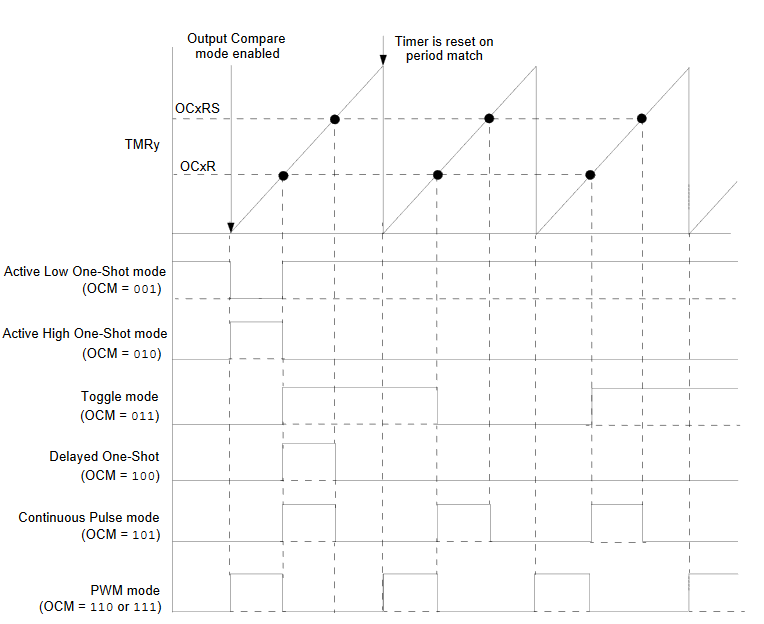
\includegraphics[width=0.9\textwidth]{Pictures/output compare.png}
    \caption{Fonctionnement de l'\textit{output compare}}
    \label{fig:enter-label}
\end{figure}

\section{Mesure de position}

La détermination de la distance parcourue par une roue est déterminée à l'aide du \textit{QEI}. Les roues comptant 360 fentes, un tour complet de roue correspond à une valeur de 1440 dans le registre de sortie du \textit{QEI}, \textbf{POSxCNT} \ref{clk_to_cm}. Puisque la valeur de ce registre est susceptible d'atteindre des grandes valeurs tant positives que négatives, \textit{POSxCNT} est remis à $0x8000$ (la moitié d'un stockage à $16$ bits) avant chaque exécution de commande évitant ainsi les \textit{underflow} ou les \textit{overflow}. Pour la régulation en rotation, on passe de la distance à l'angle grâce à \ref{cm_to_ang}.

\begin{equation}
    d = \frac{POSxCNT \times 2 \times \pi}{1440}
    \label{clk_to_cm}
\end{equation}
\begin{equation}
    \alpha = \frac{d \times 180}{E \times \pi}
    \label{cm_to_ang}
\end{equation}

Où $d$ est la distance parcourue, $\alpha$ l'angle effectué par le robot et $E$ son empatement.

\section{Génération de consigne}
\label{chap:consigne}
Il a été choisi de calculer à l'avance la position du robot lors de la phase d'accélération et de décélération sans stocker la position désirée lors du MRU (voir fig \ref{consigne}). Ceci permet d'avoir une liste de positions dont la taille est fixée par l'accélération et la vitesse maximale puisque le temps total sera égal à $2\frac{v_{max}}{a}$. Pour réduire le nombre de calculs nécessaires, la seconde partie de la consigne n'est que la distance finale à laquelle on soustrait le début de la consigne. On ajoute aussi à la fin de la liste de commande la distance finale pendant 15 centièmes de seconde pour être certain que le robot ait atteint son objectif avant de s'arrêter.

\begin{figure}[H]
    \centering
    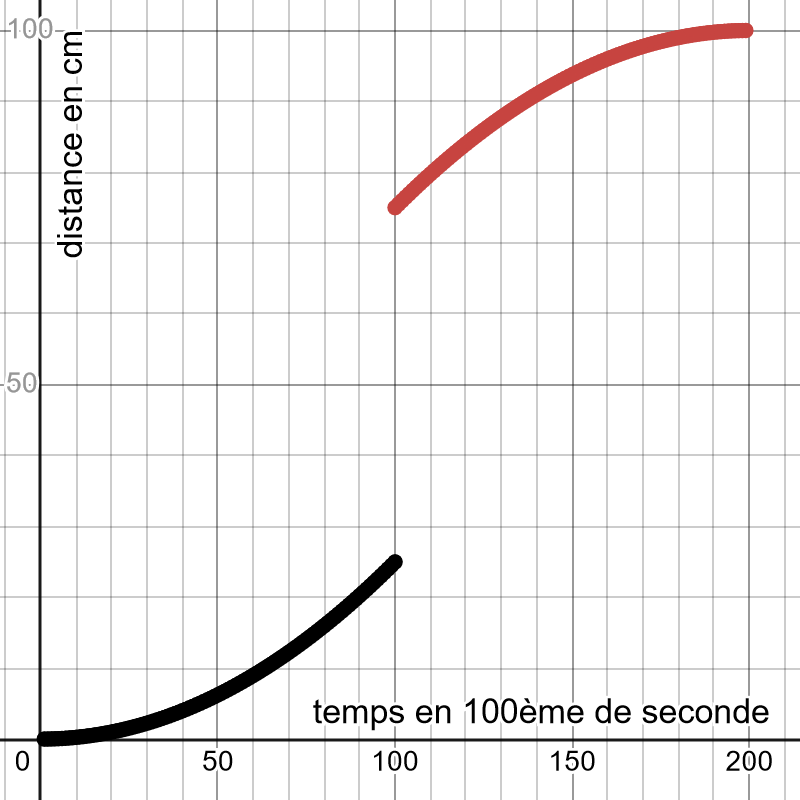
\includegraphics[width=0.9\textwidth]{Pictures/consigne.png}
    \caption{consigne pour une translation de 100 cm}
    \label{consigne}
\end{figure}

\section{Régulateur en translation}

La mise en place du régulateur est facilement réalisable à partir du schéma fonctionnel (fig : \ref{fig:regulateur_translation}). La première difficulté rencontrée a été de régler le \textit{timer} pour qu'il fonctionne à $100Hz$. Puisqu'avec la fréquence de fonctionnement du dsPIC $f_{\mu C} = 40\times10^6 Hz$, il aurait fallu qu'il compte jusqu'à $\frac{40\times10^6}{100}-1 = 399999$, or la valeur de réglage du \textit{timer} est sur 16 bits donc on ne peut pas dépasser $2^{16} = 65536$. on a donc pris $PR = 57143$ et on n'utilise le régulateur qu'après que le \textit{timer} ait "sonné" 7 fois.

\begin{figure}[H]
    \centering
    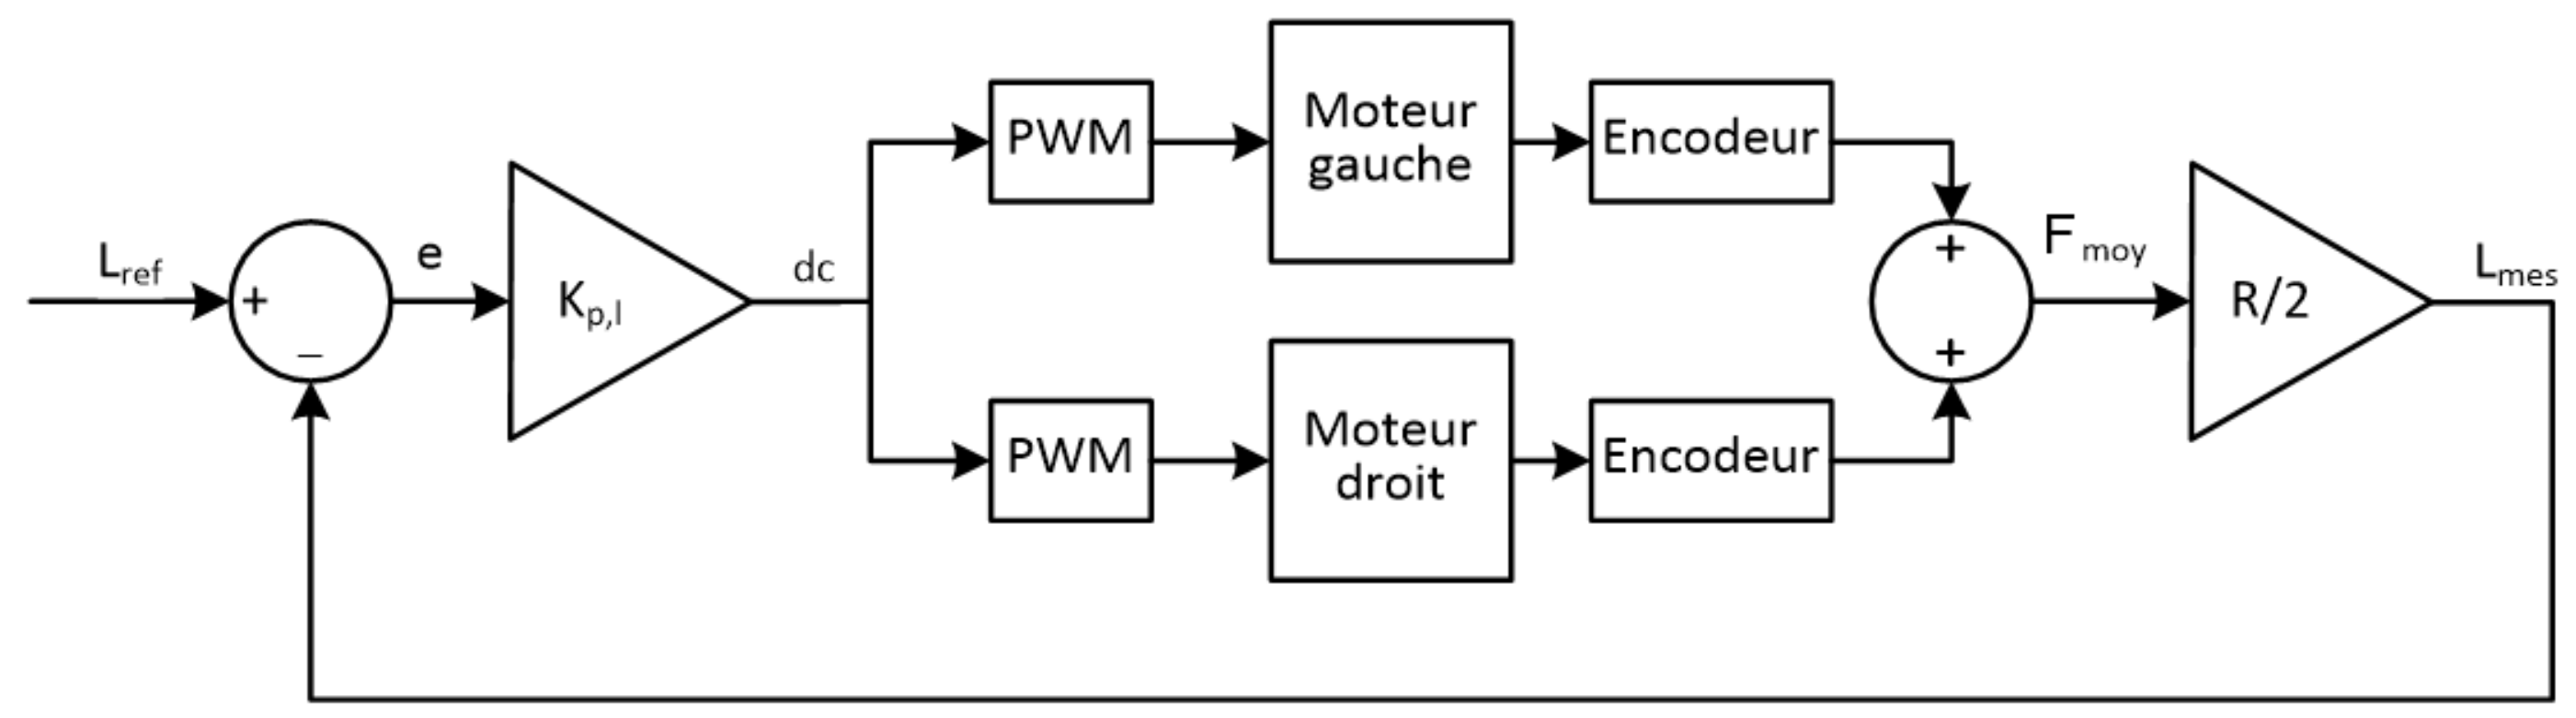
\includegraphics[width=0.9\textwidth]{Pictures/regul_trans.png}
    \caption{Fonctionnement du \textit{Régulateur en translation}}
    \label{fig:regulateur_translation}
\end{figure}

L'autre point complexe a été qu'il n'y a pas de consigne pour la phase à laquelle le robot est à vitesse constante (comme expliqué \ref{chap:consigne}). La commande envoyée au moteur n'est donc pas modifiée pendant tout le temps où le robot est en MRU. Pour savoir quand se remettre à suivre la consigne, le microcontrôleur compare son ancienne commande de vitesse avec celle qu'il devrait appliquer si la consigne était celle du début de la décélération (en valeur absolue). Si la nouvelle commande est inférieure à l'ancienne, il reprend sa régulation en MRUA.\\
Comme on peut le voir dans le code (annexe \ref{code:mouvement}), la variable \textit{t} sert de temps. Elle est utilisée pour savoir à quelle valeur de la consigne on est censé être et elle est incrémentée à chaque fois que la commande est modifiée. Quand la phase d'accélération est terminée, on arrête d'incrémenter \textit{t} tous les centièmes de secondes. On recommence à augmenter \textit{t} quand le robot arrive dans sa phase de décélération.

\section{Régulateur en rotation}

\subsection{Modélisation du robot en rotation}

Tout comme pour la régulation en translation, il faut déterminer le modèle du robot en rotation pour dimensionner le régulateur proportionnel. Pour ce faire, on mène une série d'expériences (identiques à celles de la régulation en translation) dont les résultats sont affichés sur les figures \ref{fig:statrot} \& \ref{fig:approxrot}

\begin{figure}[H]
    \centering
    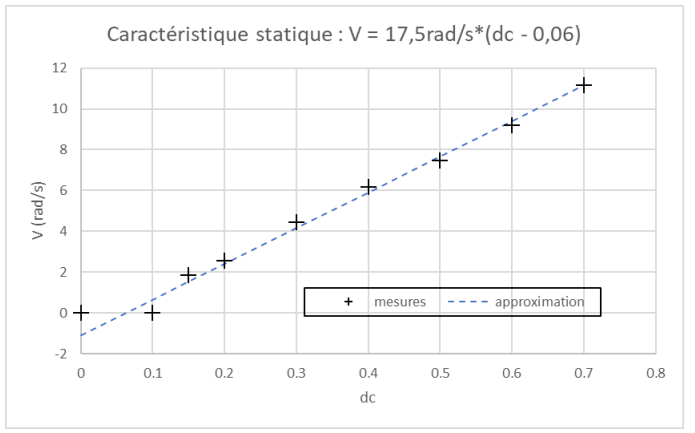
\includegraphics[width=0.9\textwidth]{Pictures/caracstatrot.png}
    \caption{Caractéristique statique en rotation}
    \label{fig:statrot}
\end{figure}

\begin{figure}[H]
    \centering
    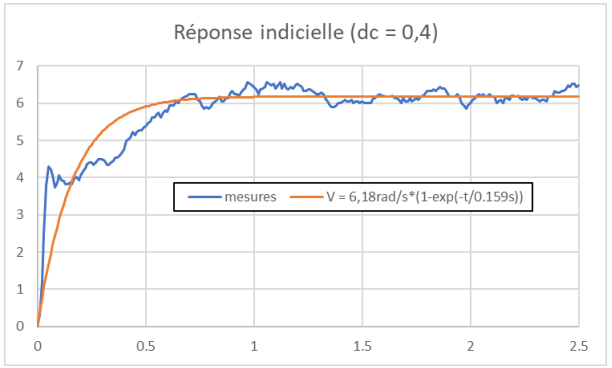
\includegraphics[width=0.9\textwidth]{Pictures/approxreponstati.png}
    \caption{Approximation de la réponse indicielle pour dc=0.3}
    \label{fig:approxrot}
\end{figure}

On peut modéliser le robot en rotation par la fonction de transfert suivante, qui est identique dans la forme à celle du robot en translation : 
\begin{align*}
H_r(p)&=\frac{V(p)}{U(p)}=\frac{k_r}{(1+p \tau)} \frac{1}{p}
\end{align*}

La pente de la droite sur la caractéristique statique sur la figure \ref{fig:statrot} donne la valeur de $k_r$ et la constante de temps dans l'approximation de la réponse indicielle sur la figure \ref{fig:approxrot} donne la valeur de $\tau$. On peut donc réécrire la fonction de transfert de la manière suivante :

\begin{align*}
H_r(p)&=\frac{17.5}{(1+0.159p )} \frac{1}{p}
\end{align*}

Le schéma de régulation est représentée sur la figure \ref{fig:schémaregrot}. Sachant que la période d'échantillonnage vaut $\frac{1}{100 \ Hz}$, il ne reste plus que le gain $k_p$ à déterminer.

\begin{figure}[H]
    \centering
    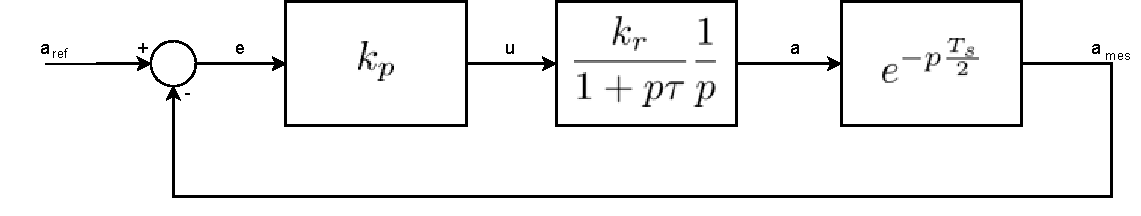
\includegraphics[width=0.9\textwidth]{pdffiles/regrot.drawio.pdf}
    \caption{Schéma de régulation en rotation}
    \label{fig:schémaregrot}
\end{figure}

\subsection{Dimensionnement du régulateur en rotation}

Le dimensionnement du régulateur se fait à partir des critères des marges de gain et de phase. Ces marges sont identiques à celles évoquées dans la régulation en translation puisque les modèles des 2 régulateurs sont similaires.

\subsubsection{Marge de gain}

L'expression du gain est : 

\begin{align*}
    k_{p1} &= \frac{\omega_1 \sqrt{1 +(\omega_1 \tau)^2 }}{2 k_r}
\end{align*}

Où on a besoin de trouver la valeur de $\omega_1$. On peut la déduire à partir de l'équation suivante :

\begin{align*}
    \text{Atan}(\omega_1 \tau)+ \omega_1 \frac{T_s }{2}=\frac{\pi}{2} 
\end{align*}

A l'aide du site internet \url{https://www.geogebra.org/calculator}, on trouve graphiquement la valeur de $\omega_1$ sur la figure \ref{fig:omega1} et elle vaut $35.28 \ rad/s$.

\begin{figure}[H]
    \centering
    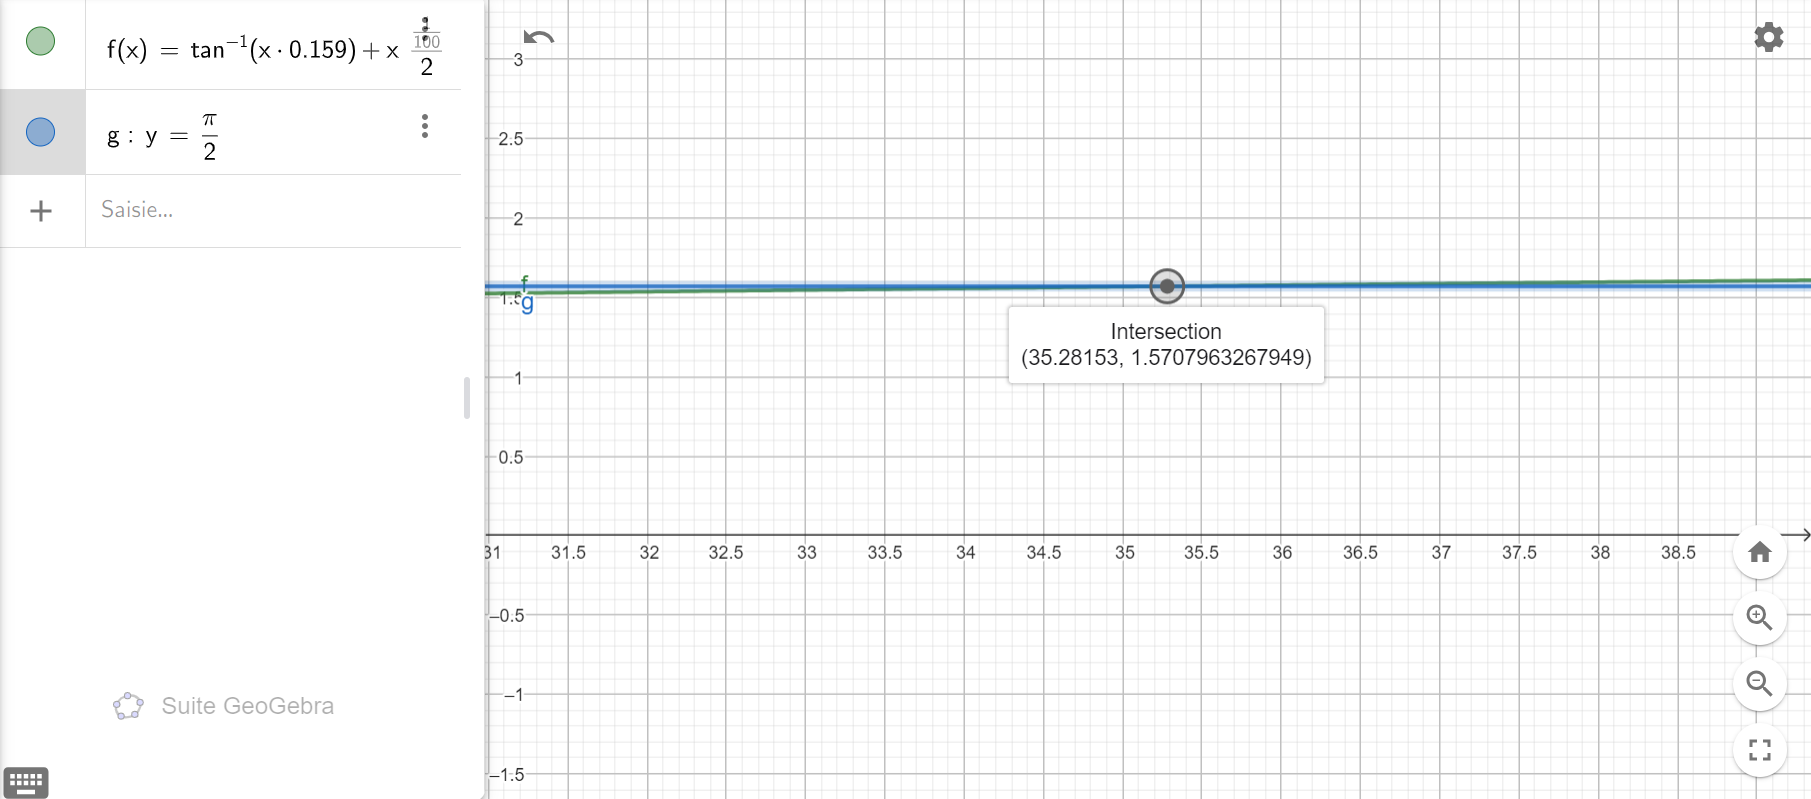
\includegraphics[width=0.9\textwidth]{Pictures/omega_1_marge_gain.png}
    \caption{Résolution graphique pour déterminer $\omega_1$}
    \label{fig:omega1}
\end{figure}

Ainsi, on peut calculer la valeur de $k_{p1}$ :

\begin{align*}
     k_{p1} &= \frac{35.28 \sqrt{1 +(35.28 \cdot 0.159)^2 }}{2 \cdot 17.5} \\
     &= 5.74354 \ rad^{-1}
\end{align*}

\subsubsection{Marge de phase}

L'expression du gain est : 

\begin{align*}
    k_{p2} &= \frac{\omega_2 \sqrt{1 +(\omega_2 \tau)^2 }}{ k_r}
\end{align*}

On a besoin de trouver la valeur de $\omega_2$. On peut la déduire à partir de l'équation suivante :

\begin{align*}
    arctg(\omega_2 \tau)+ \omega_1 \frac{T_s }{2}=\frac{\pi}{3} 
\end{align*}

Comme avant, on trouve graphiquement la valeur de $\omega_2$ sur la figure \ref{fig:omega2} et elle vaut $9.7605 \ rad/s$.

\begin{figure}[H]
    \centering
    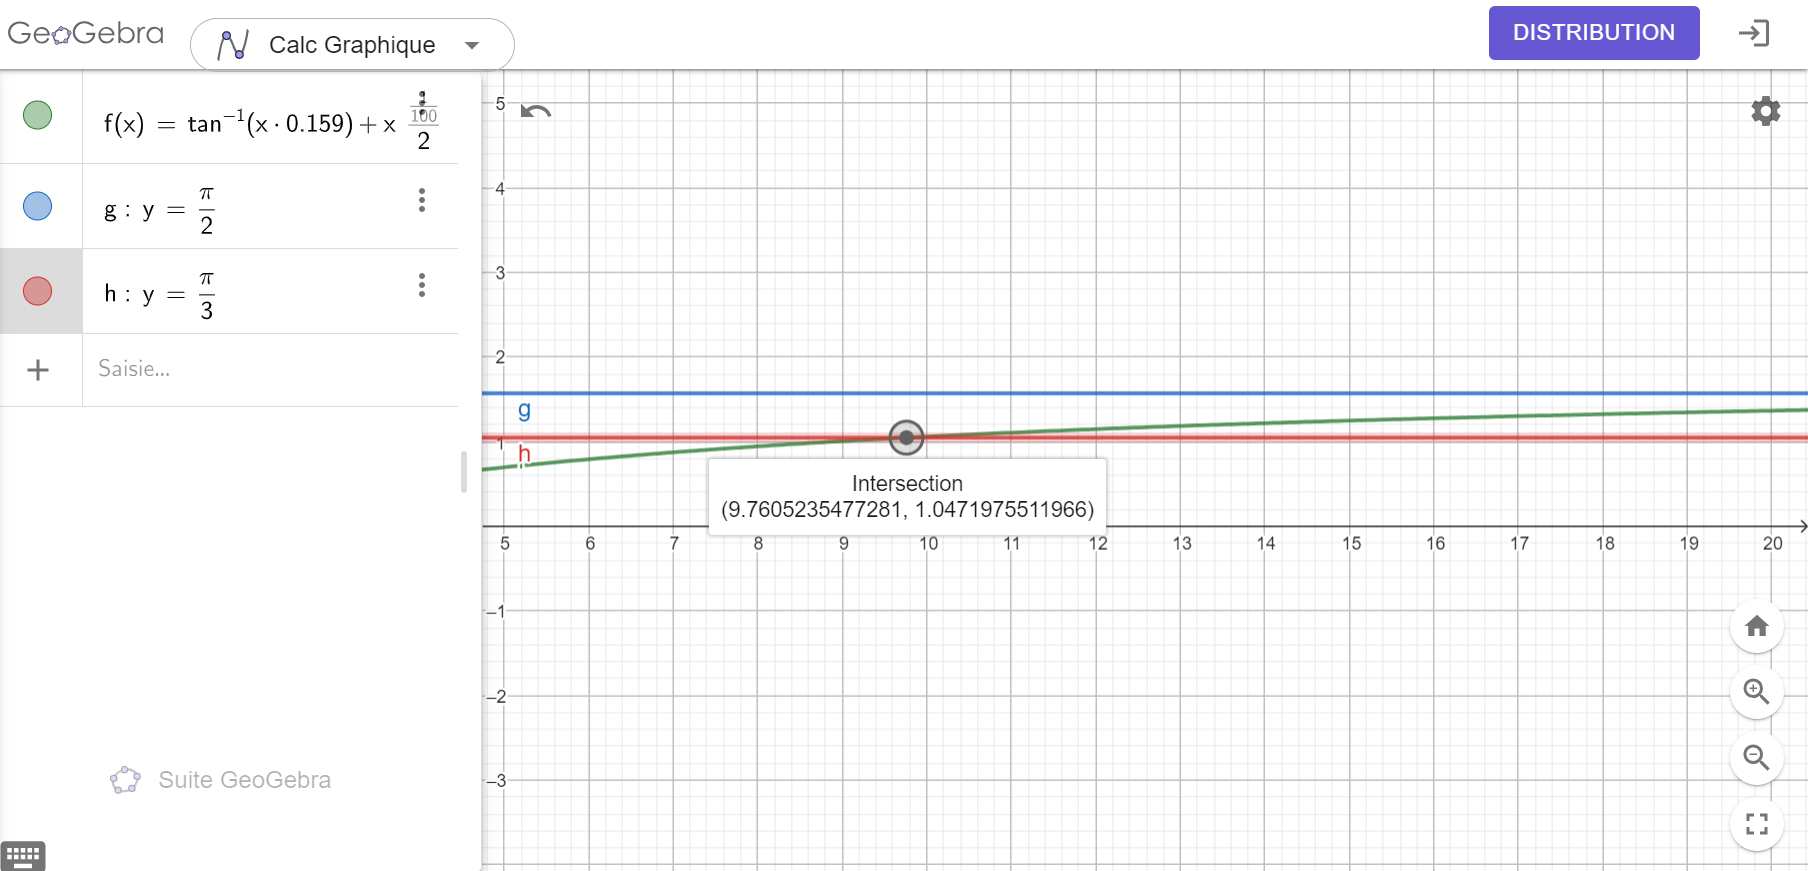
\includegraphics[width=0.9\textwidth]{Pictures/omega_2_marge_phase.png}
    \caption{Résolution graphique pour déterminer $\omega_2$}
    \label{fig:omega2}
\end{figure}

Ainsi, on peut calculer la valeur de $k_{p2}$ :

\begin{align*}
     k_{p1} &= \frac{9.7605 \sqrt{1 +(9.7605 \cdot 0.159)^2 }}{ 17.5} \\
     &= 1.0297\ rad^{-1}
\end{align*}

\subsubsection{Valeur finale du gain}

Il faut choisir le plus petit gain et il s'agit de $k_{p2}$. Cependant puisqu'on travaille en degré, il faut changer les unités du gain :
\begin{align*}
     k_{p1} &= 1.0297\ rad^{-1} \\
     &= 0.017971 \ \text{°}^{-1}
\end{align*}


\section{Régulateur complet}

La génération de consigne a simplement demandé l'ajout d'une liste contenant les commandes en rotation. Sur base du schéma en bloc donné sur \href{https://gitlab.com/mosee/elech309-2024}{gitlab}, le code a été modifié afin d'inclure les 2 régulateurs.

\begin{figure}[H]
    \centering
    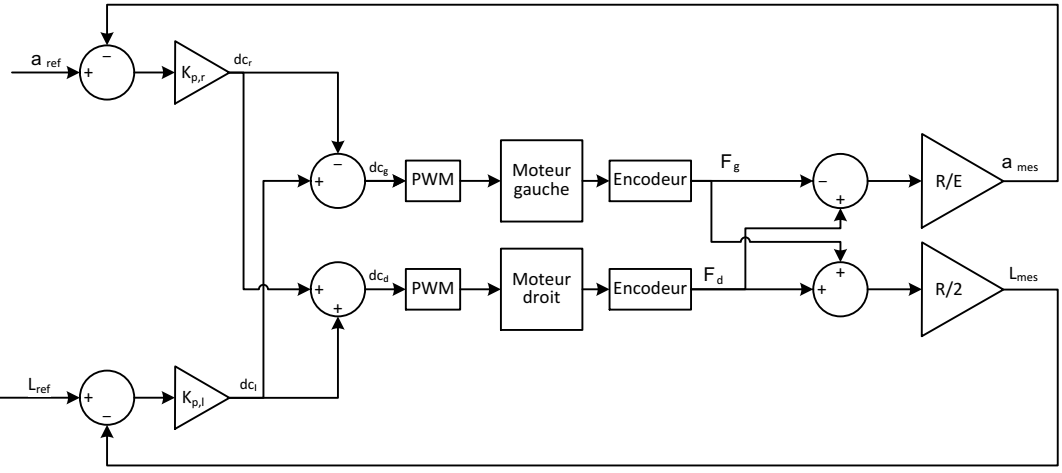
\includegraphics[width=0.9\textwidth]{Pictures/regul_pol.png}
    \caption{Fonctionnement du \textit{Régulateur en translation}}
    \label{fig:enter-label}
\end{figure}

La plus importante des modifications à effectuer a été d'ajouter un régulateur en MRU là où la consigne n'était pas modifiée précédemment, de manière à empêcher le robot de tourner en ligne droite ou d'avancer lors d'une rotation.

\section{Vérification du code}

Certaines sections du code ont été légèrement modifiées pour s'exécuter sur un ordinateur, de façon à vérifier leur bon fonctionnement. Dans cette partie qui ne s'intéresse qu'au mouvement, la seule fonction qui est implémentable est la génération de consigne, qui est en annexe (\ref{code:test_consigne}) et qui a permis de s'assurer que les listes de positions et d'angles soient correctes quelle que soit la commande.


\chapter{Traitement des signaux audio}

Sur base de l'étude de la communication audio, disponible dans le \href{https://gitlab.com/mosee/elech309-2024}{gitlab du projet}, cette partie du projet concerne la réalisation :

\begin{enumerate}
    \item[$\bullet$] d'un signal modulé en fréquence et suivant un format de trame donné
    \item[$\bullet$] d'une chaîne d'acquisition
    \item[$\bullet$] de la démodulation du signal
    \item[$\bullet$] de l'appel à la fonction qui exécute la commande\footnote{Cette fonction a été écrite précédemment, elle fait partie de la partie mécanique du projet. On doit juste passer en argument le signal démodulé}
\end{enumerate}

Nous n'avons pas besoin de réaliser le premier point puisque des exemples de signaux sont déjà disponibles sur l'UV. Par ailleurs, on peut remarquer que contrairement à ce qui est conseillé, on a décidé d'utiliser un seul dsPIC. Tout ceci est repris sur la Figure \ref{fig:bloc_com}

\begin{figure}[H]
    \centering
    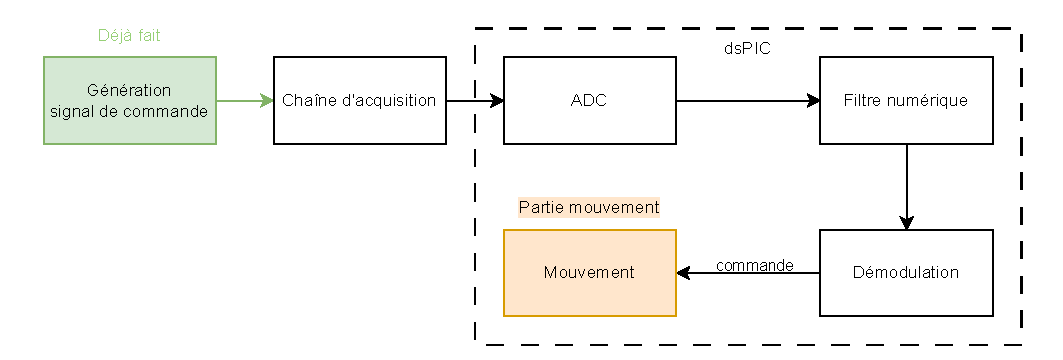
\includegraphics[scale=0.8]{pdffiles/diagramme_comm.pdf}
    \caption{Schéma-bloc de la partie communication}
    \label{fig:bloc_com}
\end{figure}

\section{Chaîne d'acquisition}

Avant de dimensionner notre chaîne d'acquisition, nous devons analyser les contraintes qui nous sont imposées.


Tout d'abord, le capteur est un microphone de type piézoélectrique, avec un étage de sortie à transistor intégré, qu'il faut polariser avec une résistance de 2.2k$\Omega$. Le signal en sortie est un signal alternatif de 1mV d'amplitude. Il faut donc amplifier ce signal en le maintenant dans la plage de fonctionnement du dsPIC, c-à-d. entre 0V et 3.3V. Cette plage sera la même pour les ampli-op utilisés ultérieurement.

Ensuite, puisque le signal va être numérisé, il faut ajouter un filtre de garde pour éviter le repliement spectral. Le filtre de garde doit respecter les conditions suivantes : 

\begin{enumerate}
    \item[$\bullet$] Atténuation maximale des fréquences utiles : H1=0.99
    \item[$\bullet$] Atténuation minimale des fréquences repliées : H2=0.05
    \item[$\bullet$] Filtre d'ordre 2 (pour limiter le nombre d'étage de la chaîne analogique)
    \item[$\bullet$] Filtre de Butterworth (réponse la plus plate possible dans la bande passante)
\end{enumerate}

Pour finir, notons que les fréquences utiles sont $900 Hz$ et $1.1 kHz$.

Sachant tout cela, on peut distinguer les tâches suivantes que la chaîne doit réaliser :
\begin{enumerate}
    \item Supprimer la composante continue du signal d'entrée (dûe à la polarisation)
    \item Polariser le signal à 1.65V puisque l'ampli-op est alimenté entre $0V$ et $3V$
    \item Sur base de cette polarisation, amplifier le signal avec un gain de 1650/64.35 dB (le plus tôt possible dans la chaîne pour ne pas amplifier le bruit généré par les composants plus loin dans la chaine)
    \item  Filtrer le signal avant de l'envoyer à l'ADC
\end{enumerate}

Pour nous faciliter le travail, on a décidé de répartir ces tâches en deux blocs. Le premier, qu'on appellera \textbf{amplification}, s'occupe des premières tâches de la chaîne. Ainsi, c'est dans ce bloc qu'on supprimera la composante continue, qu'on polarisera le signal et qu'on l'amplifiera au maximum. Le second bloc sera entièrement réservé au \textbf{filtre de garde}, auquel on pourra éventuellement inclure un gain si nécessaire. On peut rajouter ces deux nouveaux blocs à notre schéma (voir Figure \ref{fig:bloc_chaine}).

\begin{figure}[H]
    \centering
    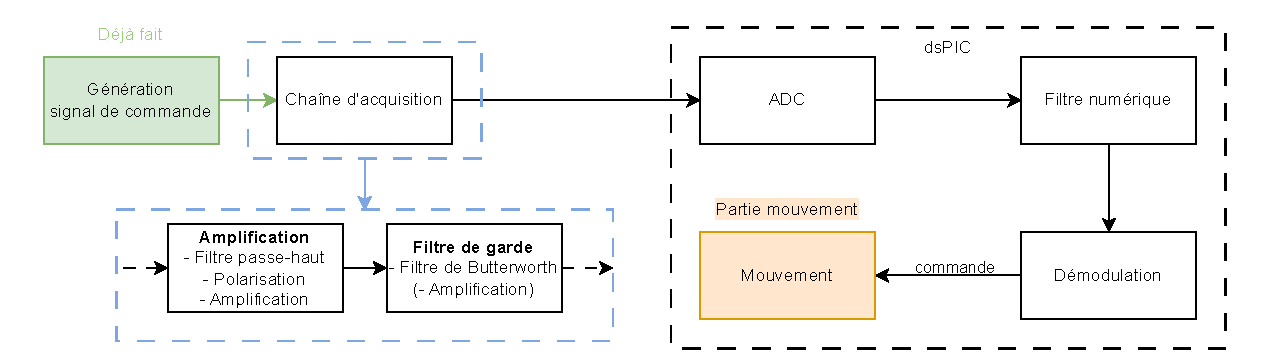
\includegraphics[scale=0.8]{pdffiles/schemabloc.pdf}
    \caption{Schéma-bloc détaillé de la chaîne d'acquisition}
    \label{fig:bloc_chaine}
\end{figure}


\subsection{Bloc Amplification}



\subsubsection{Dimensionnement}

Pour supprimer la composante continue, il suffit d'ajouter un filtre passe-haut. Nous n'avons aucune contrainte sur ce filtre, à part le fait qu'on ne doit évidemment pas atténuer les fréquences utiles. C'est pourquoi on a choisi un filtre dont la fréquence de coupure est de 90 Hz\footnote{La plus petite fréquence utile est de 900 Hz et la règle de bonne pratique est de prendre une fréquence de coupure dix fois plus petite que cette fréquence}. 

Pour dimensionner ce filtre (et le filtre de Butterworth), nous utilisons le site internet suivant : \url{https://tools.analog.com/en/filterwizard/}. 

Nous obtenons le filtre suivant sur la Figure \ref{fig:highpass}, les détails des paramètres sont disponibles dans l'annexe \ref{hfilterannexe} :

\begin{figure}[H]
    \centering
    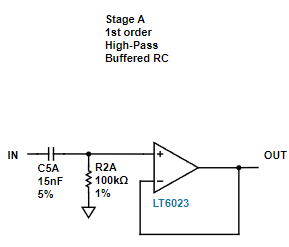
\includegraphics[width=0.4\textwidth]{Pictures/highpassfilter.png}
    \caption{Filtre passe-haut}
    \label{fig:highpass}
\end{figure}

Ce filtre est suivi d'un buffer. A partir de ce dernier, on peut déjà construire  un premier étage amplificateur. Mais avant, il nécessaire de polariser le signal car les ampli-op ont une plage de fonctionnement allant de 0V à 3.3V.

La polarisation va dépendre du type d'amplification que nous allons réaliser. Nous avons le choix entre deux types : \textbf{Amplificateur non-inverseur} ou \textbf{Amplificateur inverseur}. Le tableau \ref{tab:tabamp} reprend les caractéristiques des méthodes.

\begin{table}[H]
    \centering
    \begin{tabular}{|c|c|c|}
    \hline
        \cellcolor[RGB]{100,100,100}&\textbf{Non-inverseur} & \textbf{Inverseur} \\
        \hline
         \textbf{Gain} & $1+\frac{R_1}{R_2}$ & $-\frac{R_1}{R_2}$\\ 
         \hline
         \textbf{Impédance d'entrée} &  $\infty$& $R_2$\\
         \hline
         \textbf{Choix des résistances pour le gain} & Indépendant du filtre & Dépendant du filtre \\
         \hline
    \end{tabular}
    \caption{Tableau comparant l'amplificateur non-inverseur et inverseur}
    \label{tab:tabamp}
\end{table}

Nous allons opter pour un amplificateur non-inverseur car le gain que nous devons atteindre est très grand (plus de $60$dB) et nous avons préféré avoir la plus grande flexibilité possible dans le choix des résistances responsables de l'amplification.

La polarisation de ce type de montage se réalise en ajoutant un diviseur résistif à la borne positive de l'ampli-op. La valeur des résistances doivent être identique pour avoir une polarisation autour de $1.65\ V$ :

\begin{align*}
    1.65 &= 3.3 \ V \times \frac{R_2}{R_1+R_2}\\
    \iff R_1&=R_2
\end{align*}

On pourrait se dire que la valeur de la résistance doit être de $100 \ k \Omega$ comme indiqué dans la figure \ref{fig:highpass}. Si on fait cela, la fréquence de coupure du filtre passe-haut est décalée vers la droite car ces deux résistances sont en parallèle. Ainsi, c'est la résistance équivalente des résistances de polarisation qui doit valoir $100 \ k \Omega$ :

\begin{align*}
    R_{eq}&= \frac{R_1 \ R_2}{R_1 + R_2 }\\
    \iff 100 \ k \Omega&= \frac{R}{2}\\
    \iff R&=200 \ k \Omega
\end{align*}

Cependant, dans la série E12, il n'y a pas de résistance de $200 \ k \Omega$. On va utiliser la résistance supérieure la plus proche et elle vaut $220 \ k \Omega$. 

Le décalage de la fréquence de coupure est visible sur la courbe de Bode\footnote{Le circuit de simulation LTspice est disponible dans l'Annexe \ref{ltspiceHighPassResistors} } de la figure \ref{fig:bodehighpasspol}

\begin{figure}[H]
    \centering
    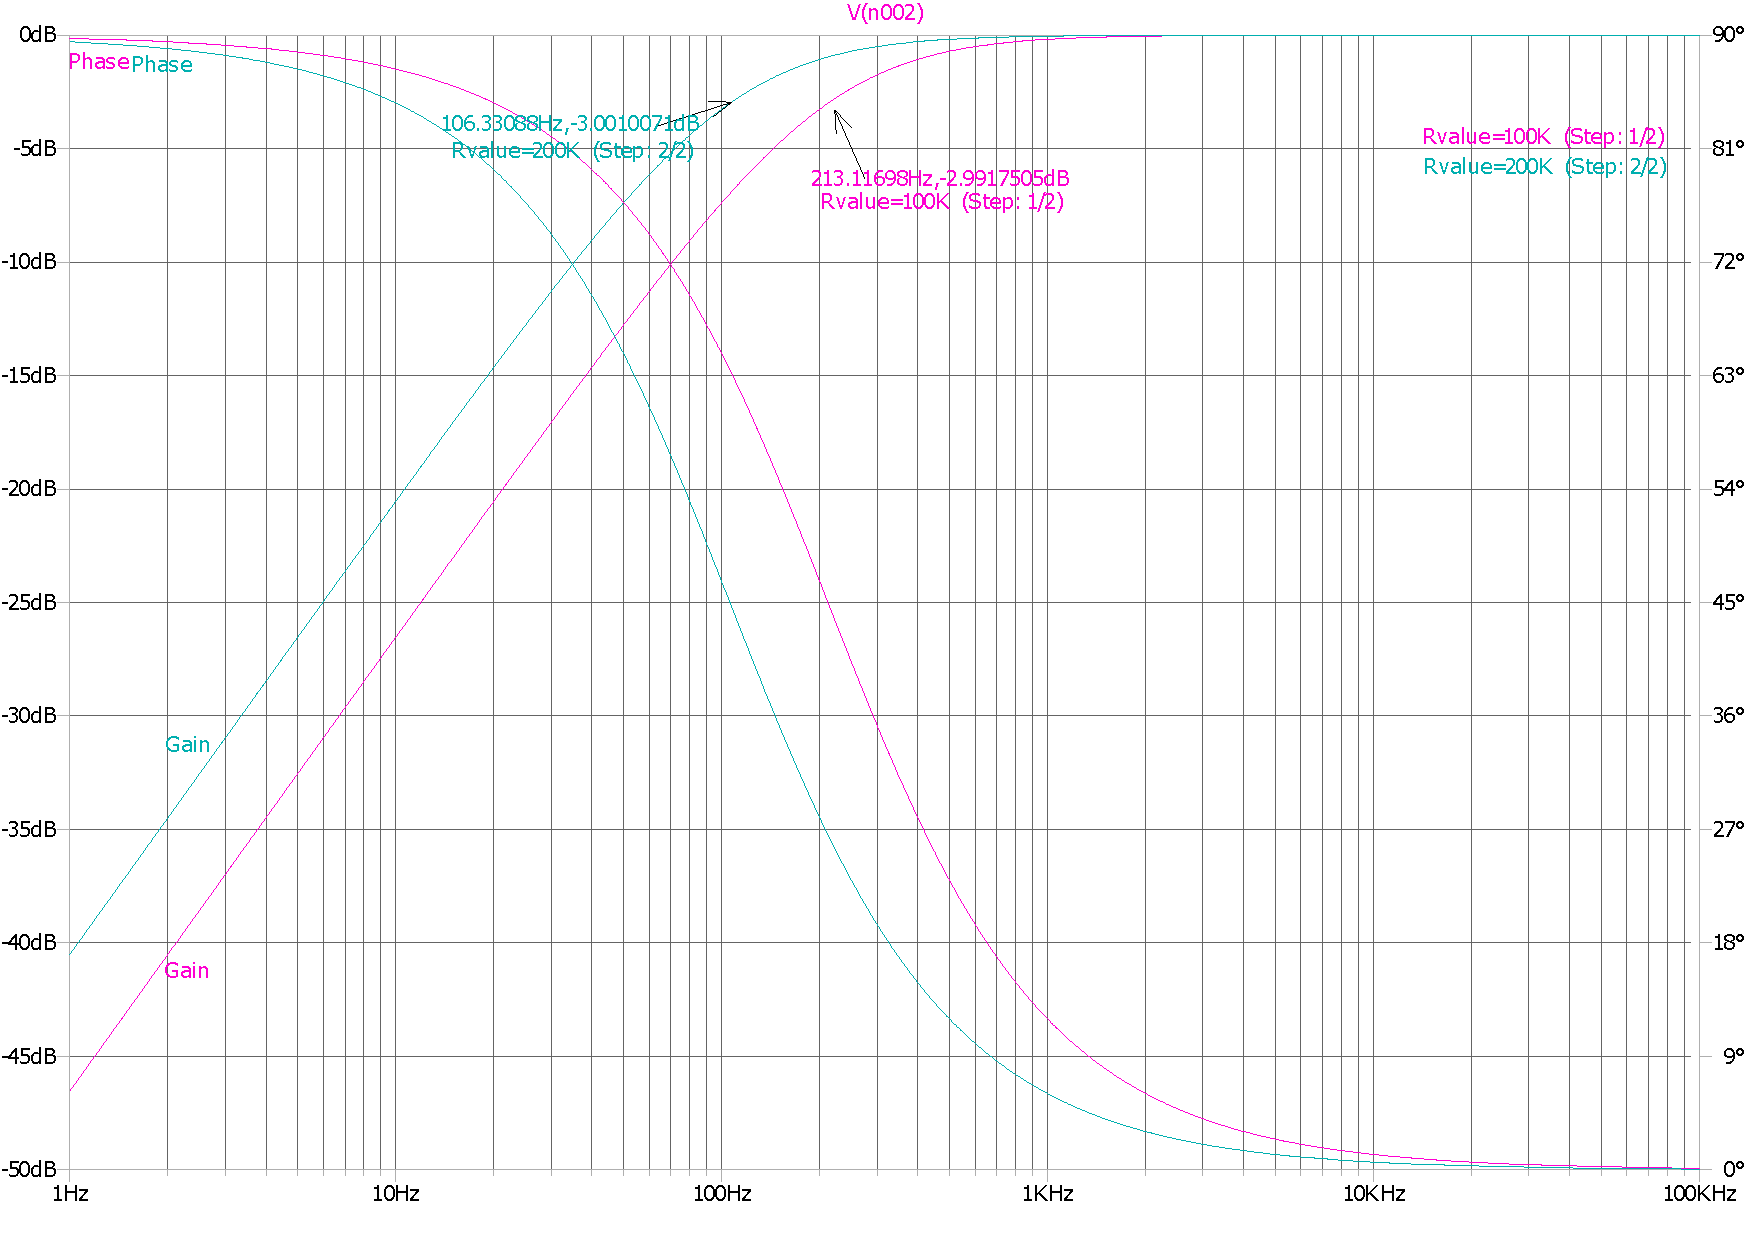
\includegraphics[width=\textwidth]{pdffiles/HighPass/BodeHighPassPolarization.pdf}
    \caption{Courbe de Bode du filtre passe-haut avec un diviseur résistif. $100 \ k \Omega $ en rose et $200 \ k \Omega$ en bleu}
    \label{fig:bodehighpasspol}
\end{figure}


La Figure \ref{fig:poldiag} représente le bloc \textbf{Amplification} après suppression de la composante continue et polarisation du signal.

\begin{figure}[H]
    \centering
    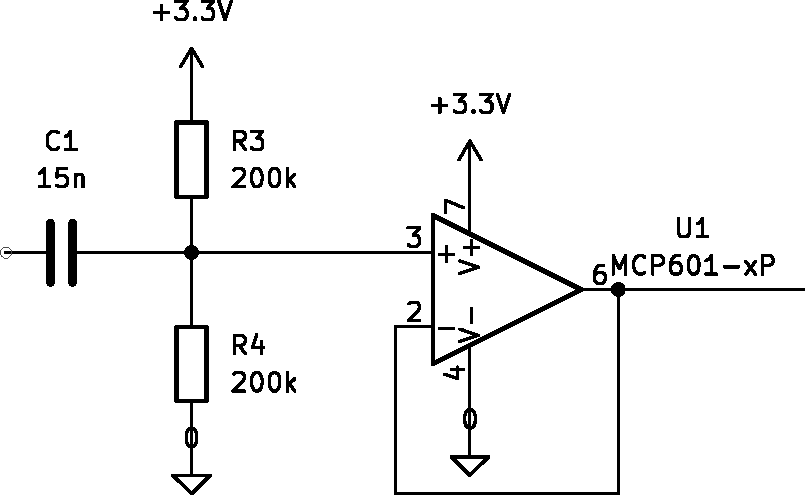
\includegraphics[width=0.5\textwidth]{pdffiles/poldiag.pdf}
    \caption{Filtre passe-haut avec polarisation}
    \label{fig:poldiag}
\end{figure}

Il ne reste plus qu'à amplifier le signal. Avant de rajouter les résistances, il faut qu'on détermine le nombre d'étage nécessaire pour obtenir le gain voulu à l'aide du produit \textbf{Gain x Bande passante}.

Le laboratoire nous fournit des ampli-op \textbf{MCP601}. Le \textbf{GBWP} de ce dernier, disponible dans la datasheet (voir annexe \ref{datasheet}), vaut $2.8 \ MHz$. Sachant que la plus haute fréquence utilisée vaut $1.1 \ kHz$, on a :

\begin{align*} 
 & \text{Gain} \times 1100 = 2.8 \times 10^{6} \\ 
\iff & \text{Gain} = \frac{2.8 \times 10^{6}}{1100}=2545.454545=68.11530 \ dB
\end{align*}

Le gain maximal d'un seul étage dans la bande passante qui nous intéresse vaut environ 2545, ce qui est au-dessus du gain  qu'on voulait obtenir. On peut donc amplifier notre signal avec un seul ampli-op. Il n'est donc pas nécessaire d'ajouter de gain dans le filtre de garde.

Pour le choix des résistances, on peut calculer le rapport entre $R_1$ et $R_2$ :

\begin{align*}
    1+ \frac{R_1}{R_2} &= 1650 \\
    \iff \frac{R_1}{R_2} &= 1649
\end{align*}

Il faut fixer la valeur de $R_2$ pour trouver celle de $R_1$. Il y a trois choses à prendre en compte :

\begin{itemize}
    \item [$\bullet$] La résistance $R_2$ ne doit pas être trop grande (en dessous de 10k)
    \item [$\bullet$] On doit utiliser les résistances à notre disposition (la série E12)
    \item [$\bullet$] La résistance $R_2$ doit faire en sorte que son rapport avec la capacité de sortie soit le même que celui du filtre en amont.
\end{itemize}

Le dernier point concerne l'ajout d'une capacité à la sortie de l'ampli-op. En effet, si on ajoute des résistances pour le gain, la polarisation ne sera plus la même car il y a aura une chute de potentiel. On doit rajouter une capacité à la sortie de l'étage pour conserver cette polarisation. Le rapport entre la résistance $R_2$ et la capacité de sortie doit être la même que le rapport du filtre à l'entrée\footnote{Pour ne pas atténuer les fréquences utiles}. Le tableau \ref{tab:tabres} reprend les valeurs que nous avons choisies avec une brève justification.

\begin{table}[H]
    \centering
    \begin{tabular}{|c|c|l|}
    \hline
        \cellcolor[RGB]{100,100,100}&\textbf{Valeur} & \textbf{Justification} \\
        \hline
         \textbf{$R_1$} & $2.473520 \ M \Omega$ & Normalement il faudrait $2.473500 \ M \Omega$  mais la valeur choisie reste très proche.\\ 
         && On l'obtient en mettant en série les résistances suivantes : \\
         && $2.2 \ M\Omega$ ; $270 \ k\Omega$ ; $3.3 \ k\Omega$ ; $220 \ \Omega$ \\ 
         \hline
         \textbf{$R_2$} & $1.5 \ k \Omega$ & Pour avoir une résistance $R_1$ réalisable à l'aide de la série E12, 
          \\ &&$R_2$ doit valoir $1.5 \  X \Omega$. L'ordre de grandeur X est déterminé 
           \\ &&par la capacité de sortie car on ne peut pas avoir une capacité trop grande  \\
         \hline
         \textbf{$C_{sortie}$} & $1 \mu F$ & Pour avoir une résistance $R_1$ dans un ordre de grandeur plus petit que 10k, 
         \\ && il faut choisir une capacité entre $1 \ \mu F$\ et $10 \ \mu F$.\ \\
         \hline
    \end{tabular}
    \caption{Tableau comparant l'amplificateur non-inverseur et inverseur}
    \label{tab:tabres}
\end{table}

Finalement le bloc \textbf{Amplification} est repris sur la figure \ref{fig:blocampli} après avoir rajouté le gain :

\begin{figure}[H]
    \centering
    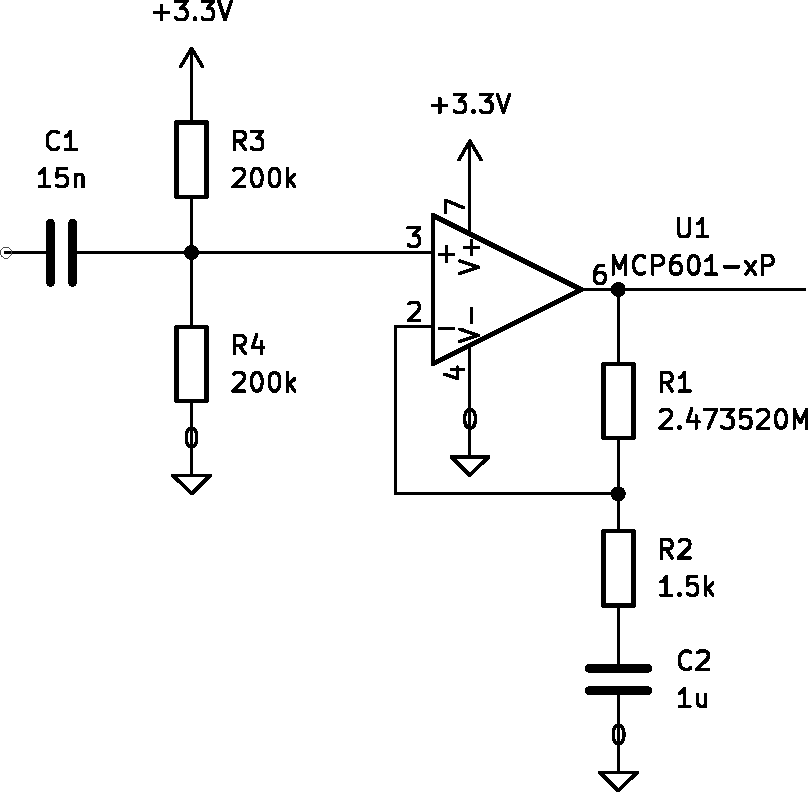
\includegraphics[width=0.5\textwidth]{pdffiles/blocampli.pdf}
    \caption{Bloc Amplification}
    \label{fig:blocampli}
\end{figure}

\subsubsection{Validation du bloc}

Après avoir dimensionné le bloc \textbf{Amplification}, il faut le tester pour valider son fonctionnement. Pour cela, il suffit d'ajouter le microphone en entrée et de mesurer à l'aide d'un Picoscope la sortie de cet étage. Le signal de sortie doit avoir l'allure suivante : un signal sinusoïdal variant de $0 \ V$ à $3.3 \ V$, centré en $1.65 \ V$.




\subsection{Bloc Filtre de garde}


\subsubsection{Dimensionnement}

Comme pour le filtre passe-haut, on va utiliser le site internet \url{https://tools.analog.com/en/filterwizard/} pour dimensionner le filtre de garde. Nous avons cependant besoin d'introduire des informations concernant la "Passband region" et la "Stopband region", toutes les deux définies par une fréquence et un gain. Elles peuvent être déduites des conditions qui nous sont imposées sur le filtre. Pour rappel :

\begin{enumerate}
    \item[$\bullet$] Atténuation maximale des fréquences utiles : H1=0.99
    \item[$\bullet$] Atténuation minimale des fréquences repliées : H2=0.05
    \item[$\bullet$] Filtre d'ordre 2 (pour limiter le nombre d'étage de la chaîne analogique)
    \item[$\bullet$] Filtre de Butterworth (réponse la plus plate possible dans la bande passante)
\end{enumerate}

Sachant que la plus grande fréquence utile est $1100 \ Hz$ et que le gain d'un filtre de Butterworth d'ordre n a la forme suivante :

$$
||H(j\omega)|| = \sqrt{\frac{1}{1+\left(\frac{\omega}{\omega_c}\right)^{2n}}}
$$

On peut reformuler les contraintes :

\begin{align*}
\begin{cases}
||H(j \ 2 \pi1100 )||&=0.99 \\
||H(j \ 2 \pi f_{\text{repliement}})||&=0.05 \\
||H(j\omega)|| &= \sqrt{\frac{1}{1+\left(\frac{\omega}{\omega_c}\right)^{4}}}
\end{cases}
\end{align*}

On doit trouver la fréquence de coupure $\omega_c$ et la fréquence de repliement $f_{\text{repliement}}$ à partir de ces équations.

\begin{align*} 
||H(j2\pi 1100)|| &= \sqrt{\frac{1}{1+\left(\frac{2\pi 1100}{\omega_c}\right)^{4}}}\\
\iff ||H(j2\pi 1100)||^{2} \left(1+\left(\frac{2\pi 1100}{\omega_c}\right)^{4}\right) &= 1\\
\iff (\omega_c)^{4} &=\frac{1}{ \left(\frac{1}{||H(j2\pi 1100)||^{2}}-1\right) \frac{1}{(2\pi 1100)^{4}} }\\
\iff \omega_c&= 18309.51674 \ rad/s\\
\iff f_c &=  2914.050095 \ Hz
\end{align*}

\begin{align*} 
||H(j\omega_{\text{repliement}})|| &= \sqrt{\frac{1}{1+\left(\frac{\omega_{\text{repliement}}}{\omega_c}\right)^{4}}}\\
\iff ||H(j\omega_{\text{repliement}})||^{2} \left(1+\left(\frac{\omega_{\text{repliement}}}{\omega_c}\right)^{4}\right) &= 1\\
\iff (\omega_{\text{repliement}})^{4} &= \left(\frac{1}{||H(j\omega_{\text{repliement}})||^{2}}-1\right) {(\omega_c)^{4}} \\
\iff \omega_{\text{repliement}} &= 81831.42343 \ rad/s\\
\iff f_{\text{repliement}} &= 13023.87554 \ Hz
\end{align*}

En introduisant les valeurs suivantes pour le dimensionnement du filtre de garde :

\begin{align*}
\begin{cases}
\text{Passband region : }  f_c = 2914.050095 \ Hz & Gain=0dB \\
\text{Stopband region : }  f = 13023.87554 \ Hz  & Gain=-26.02dB
\end{cases}
\end{align*}

On obtient le filtre de la figure \ref{fig:filtregarde}. Les détails des données introduites sur le site pour le filtre sont disponibles dans l'Annexe \ref{Lowpassfilterannexe}.

\begin{figure}[H]
    \centering
    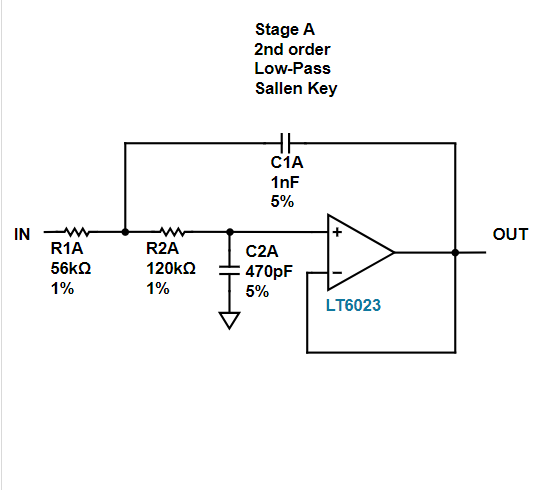
\includegraphics[width=0.5\textwidth]{Pictures/lowpass2.png}
    \caption{Filtre de Butterworth d'ordre 2}
    \label{fig:filtregarde}
\end{figure}

Le dimensionnement du filtre de garde s'arrête ici, on peut directement ajouter cet étage en cascade avec le premier et passer à la validation du bloc \textbf{Filtre de garde}.

\subsubsection{Validation du bloc}

Pour valider ce bloque indépendamment du bloc \textbf{Amplification}, on peut générer un signal sinusoïdal avec le Picoscope et observer l'atténuation du signal de sortie avec l'augmentation de la fréquence.



\subsection{Chaîne d'acquisition finale}

La figure \ref{fig:chaineacquisition} reprend la chaîne d'acquisition finale\footnote{Une version plus grande et en couleur de la chaîne est disponible dans l'Annexe \ref{chaineacquiannexe}}. On peut remarquer un ajout qui n'a pas été mentionné : il s'agit du filtre passe-bas entre l'alimentation et la polarisation du microphone et du signal avant amplification. Nous avons remarqué que le bruit du signal était important dans un milieu calme. Le filtre passe-bas permet d'atténuer ce bruit qui est en partie causé par l'alimentation.

\begin{figure}[H]
    \centering
    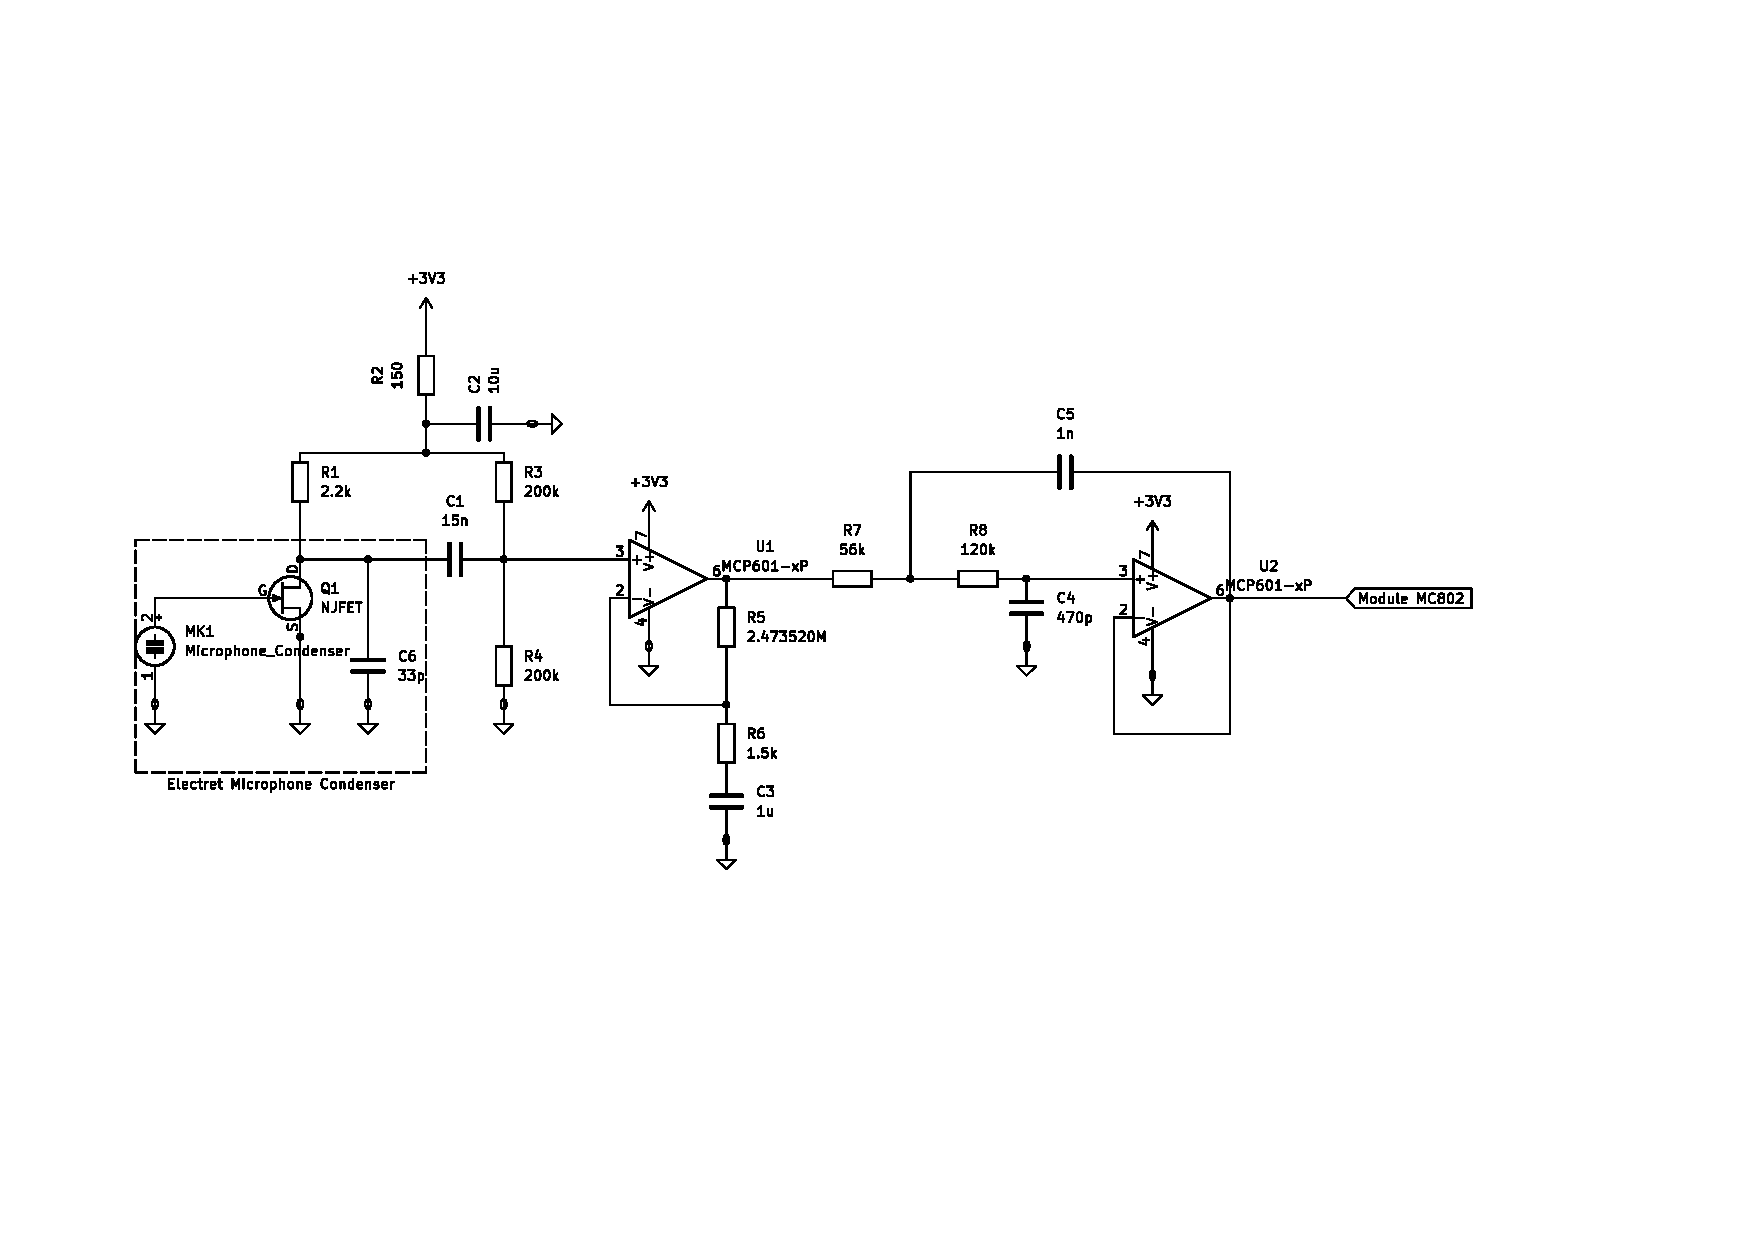
\includegraphics[width=1.2\textwidth]{pdffiles/chainacquiCompacBlack.pdf}
    \caption{Chaîne d'acquisition}
    \label{fig:chaineacquisition}
\end{figure}

\subsubsection{Validation de la chaîne d'acquisition}

Pour clôturer la section sur la chaîne d'acquisition, il faut s'assurer que cette partie du projet fonctionne correctement.
Dans un premier temps, on observe le signal de sortie de la chaîne à l'aide du Picoscope et on s'assure que les points suivants sont respectés :

\begin{itemize}
    \item [$\bullet$] Le signal est centrée en $1.65 \ V$
    \item [$\bullet$] Le signal varie de $0 \ V$ à $3.3 \ V$ pour des fréquences aux alentours de $1000 \ Hz$
    \item [$\bullet$] Le signal est atténué pour des fréquences suffisamment éloignées de $1000 \ Hz$
\end{itemize}

Sur les figures \ref{fig:sortie400}, \ref{fig:sortie900} et \ref{fig:sortie4000} se trouvent le signal après amplification en bleu et le signal de sortie final en rouge pour des signaux sonores de 400 Hz, 900 Hz et 4000 Hz. On remarque que tous les points énoncés précédemment sont respectés

\begin{figure}[H]
    \centering
    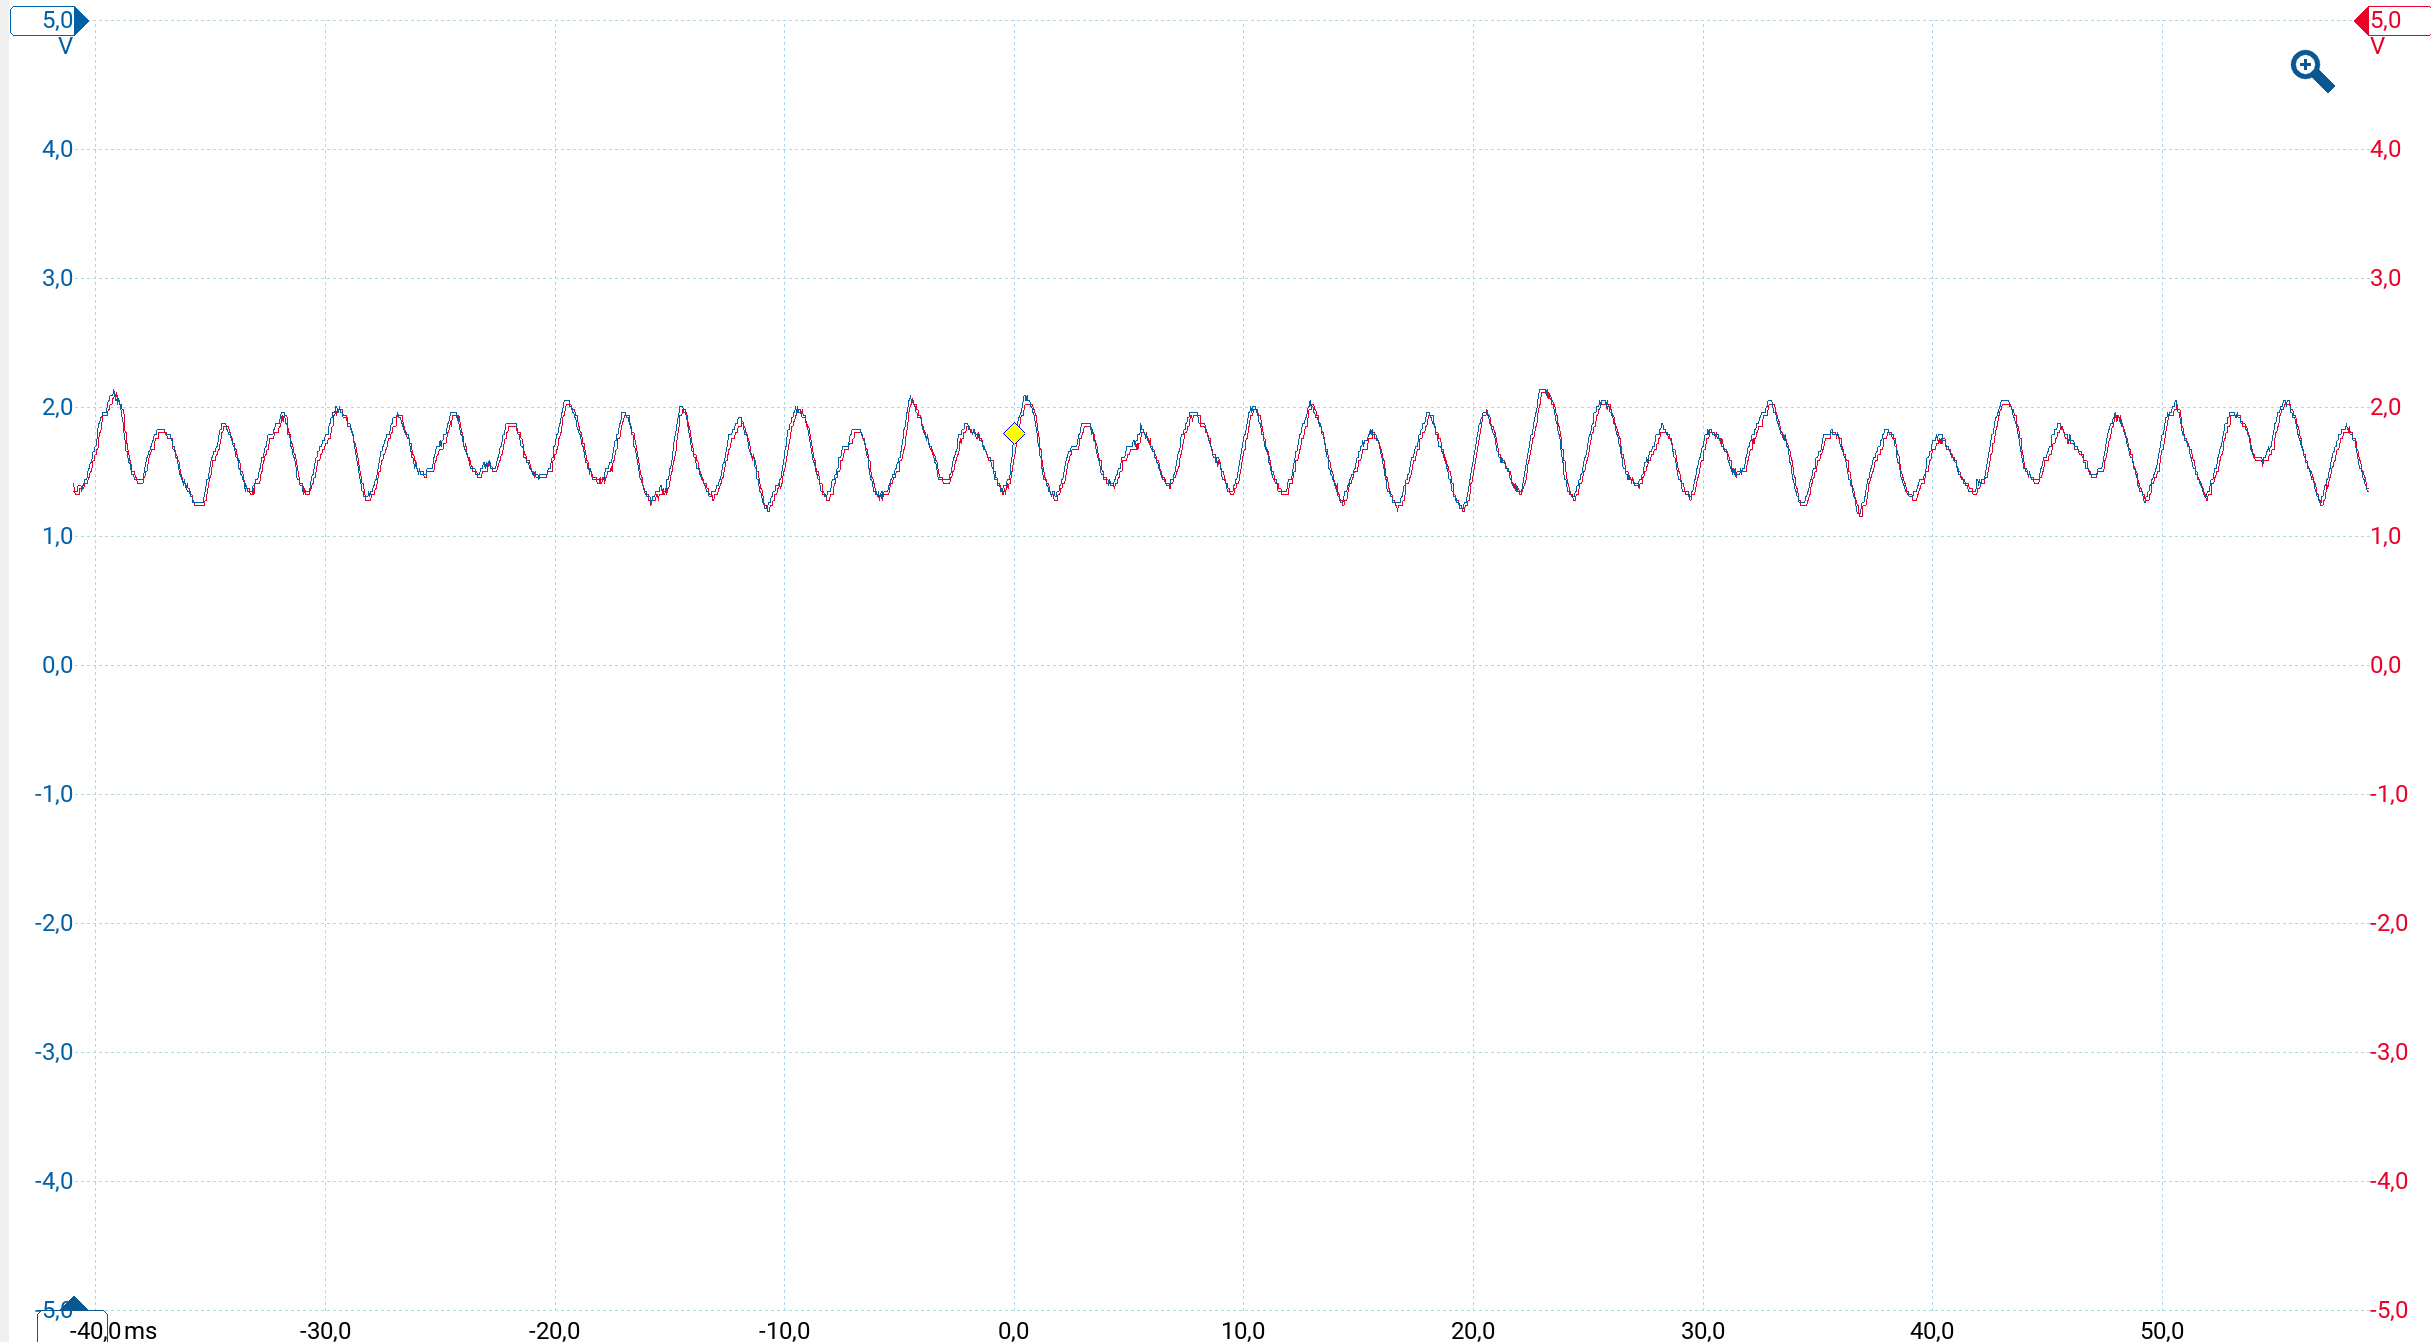
\includegraphics[width=0.6\textwidth]{Pictures/400Hz.png}
    \caption{Signal de sortie de la chaîne pour un signal audio de 400 Hz. Signal après amplification en bleu, signal de sortie final en rouge}
    \label{fig:sortie400}
\end{figure}

\begin{figure}[H]
    \centering
    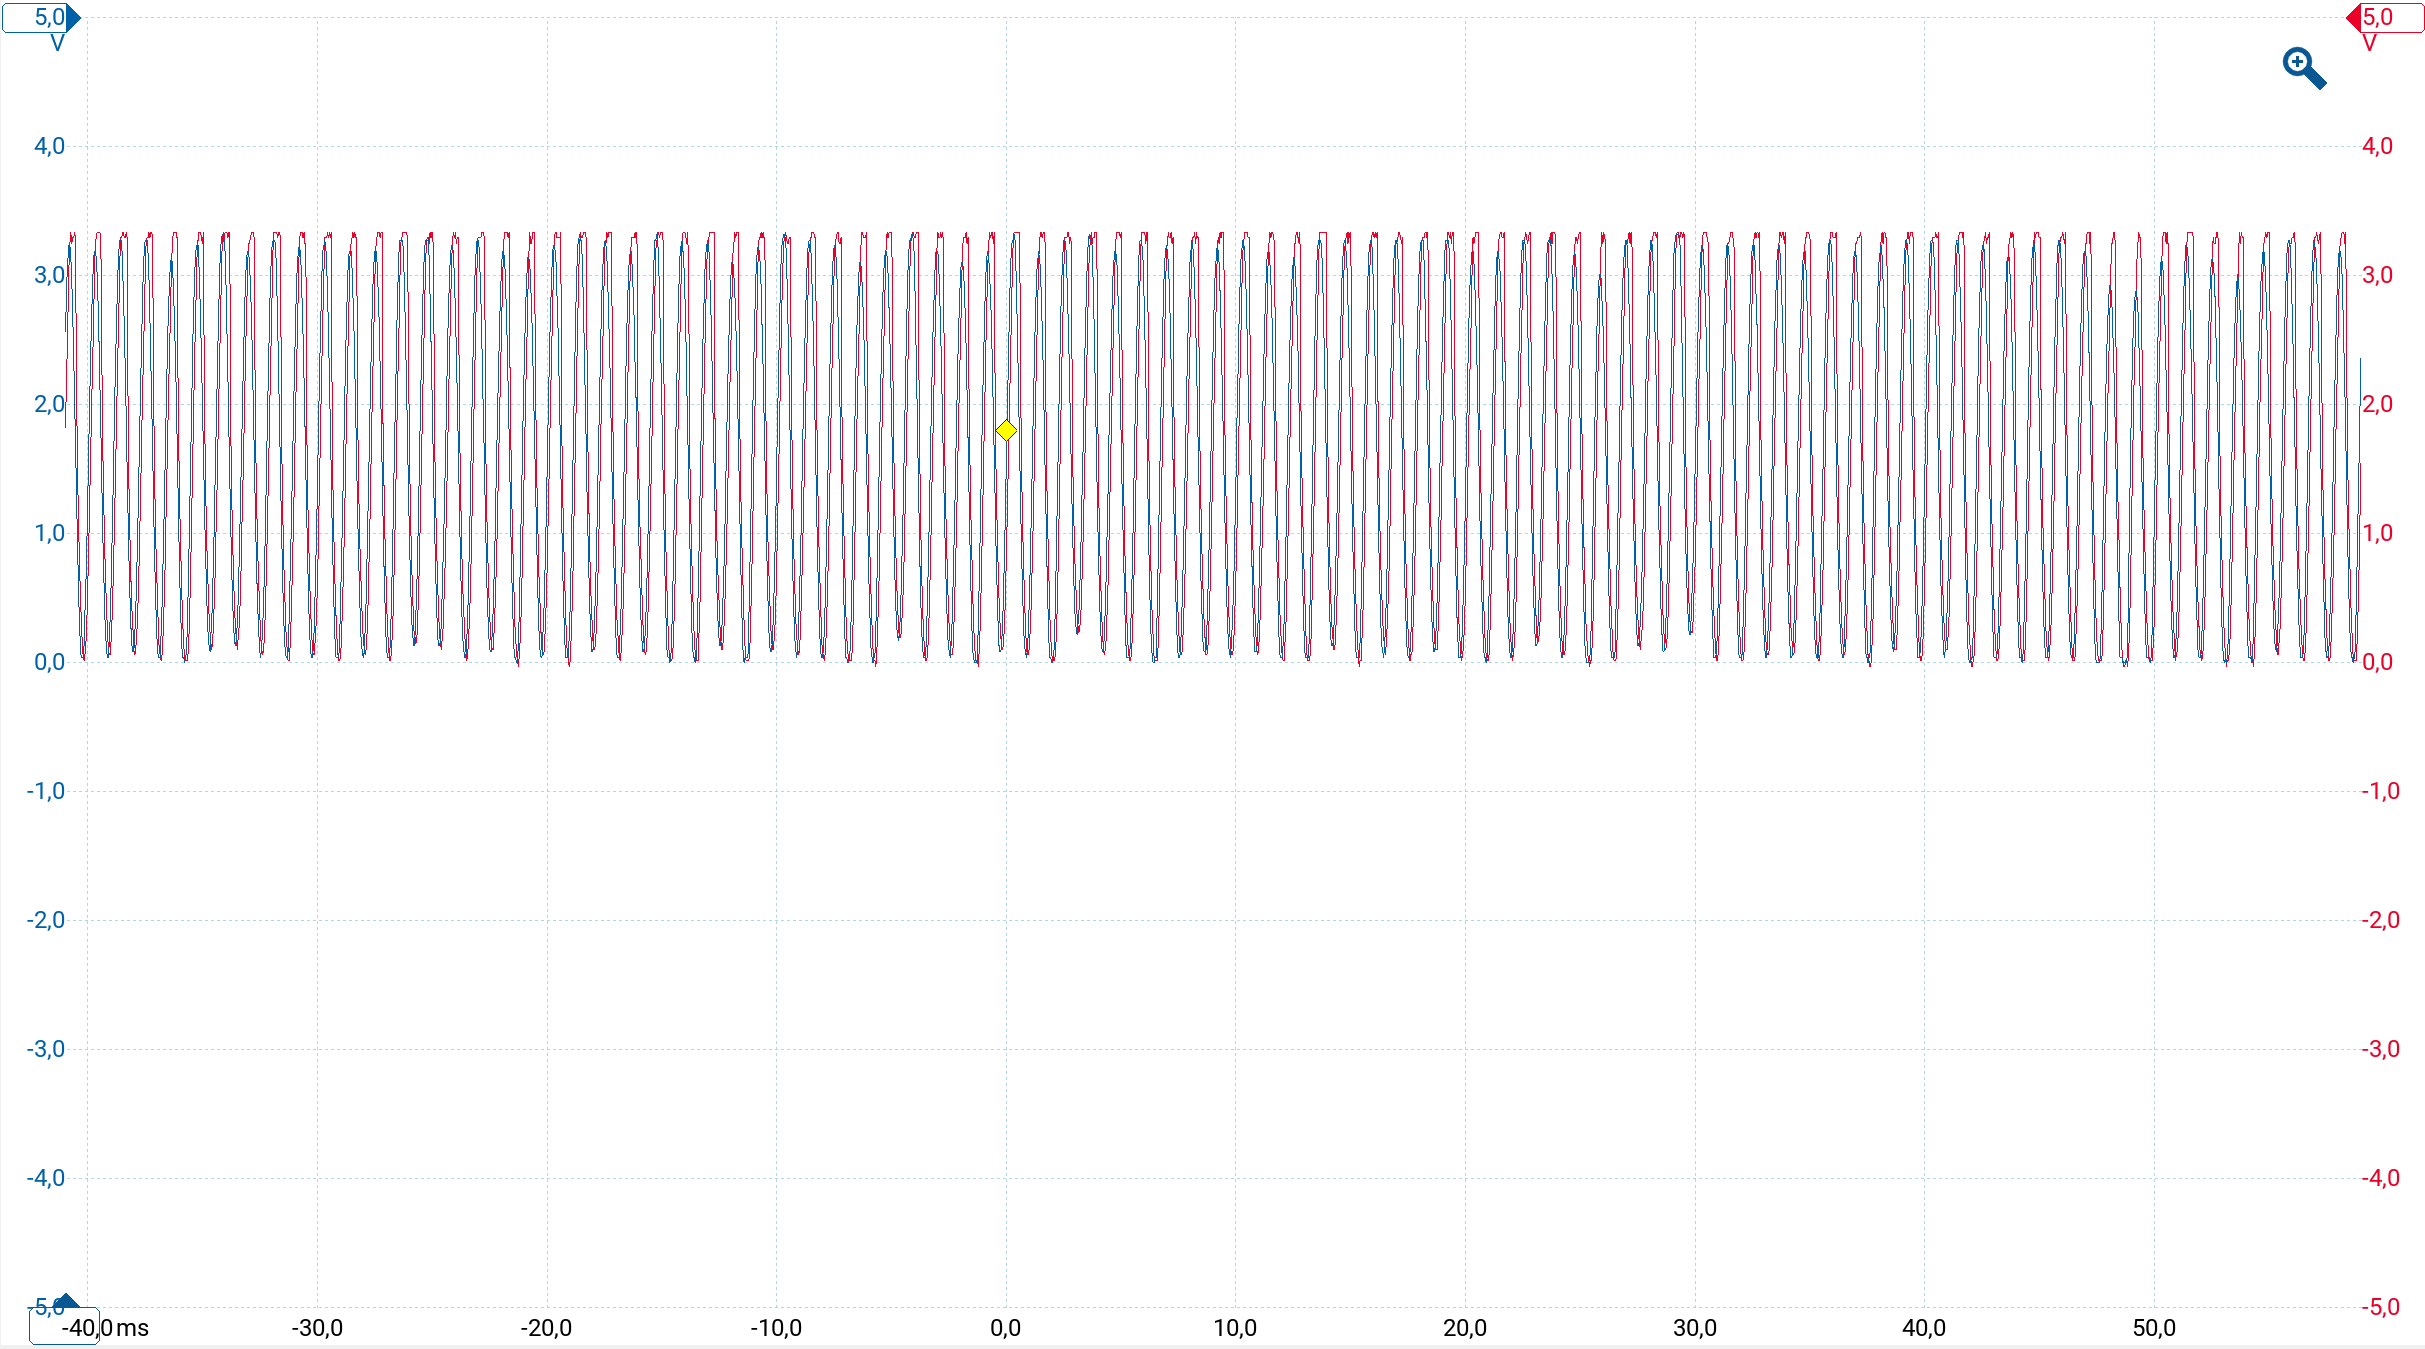
\includegraphics[width=0.6\textwidth]{Pictures/900Hz.png}
    \caption{Signal de sortie de la chaîne pour un signal audio de 900 Hz. Signal après amplification en bleu, signal de sortie final en rouge}
    \label{fig:sortie900}
\end{figure}

\begin{figure}[H]
    \centering
    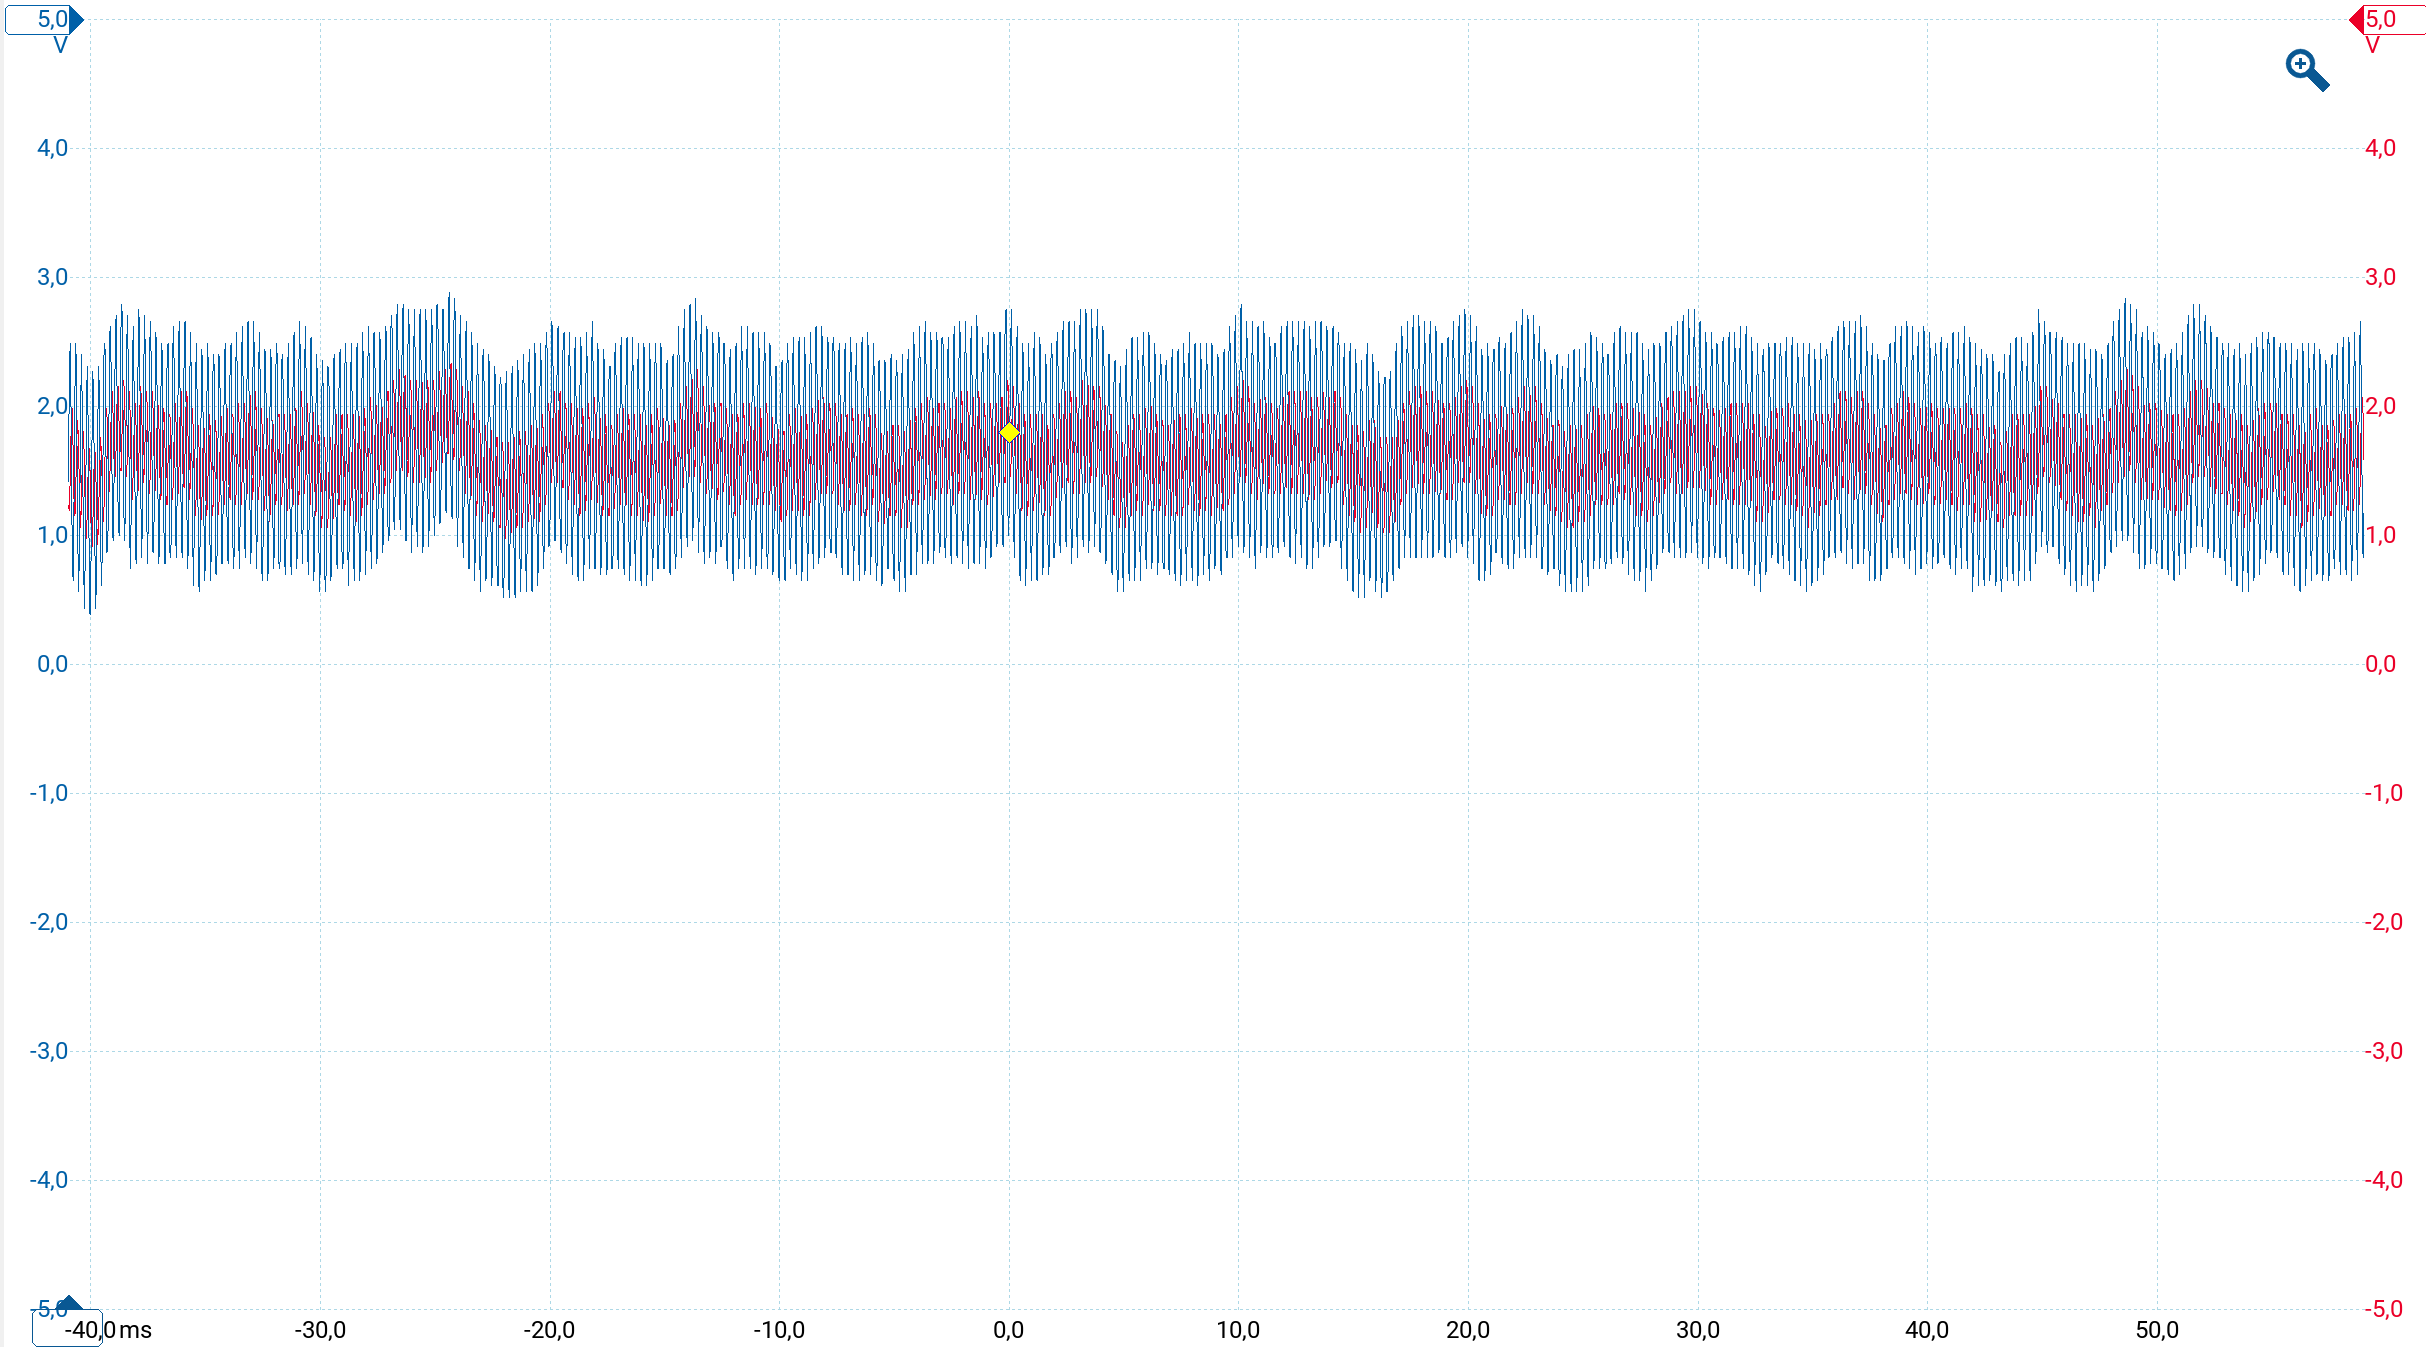
\includegraphics[width=0.6\textwidth]{Pictures/4000Hz.png}
    \caption{Signal de sortie de la chaîne pour un signal audio de 4000 Hz. Signal après amplification en bleu, signal de sortie final en rouge}
    \label{fig:sortie4000}
\end{figure}

Dans un second temps, on doit vérifier que la chaîne fonctionne pour un signal de commande audio. Pour ce faire, on utilise le \textit{canal math} du Picoscope qui affiche la fréquence du signal en fonction temps. Si on observe clairement un changement de fréquence lorsque le signal de commande audio est émis, on peut en conclure que la chaîne fonctionne correctement. La figure \ref{fig:testacqui} montre ce test et on remarque que le signal en blanc qui représente la fréquence au cours du temps varie.

\begin{figure}[H]
    \centering
    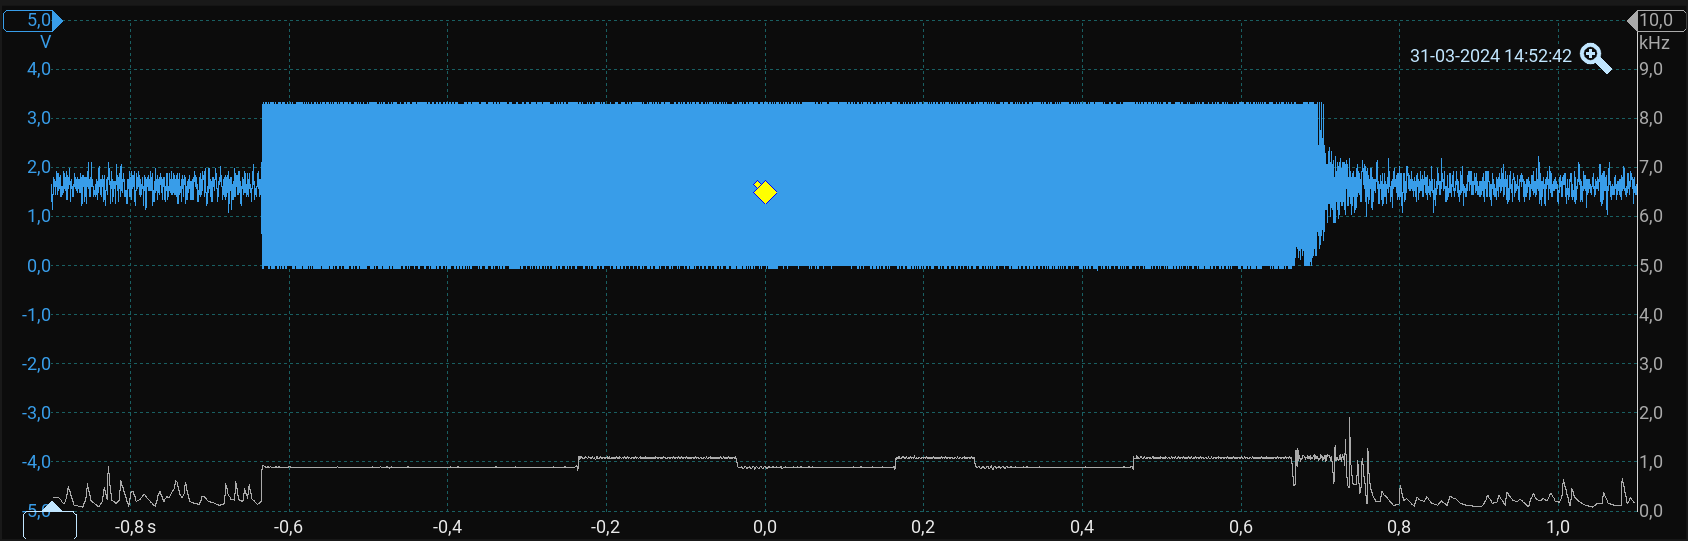
\includegraphics[width=0.8\textwidth]{Pictures/testchaineacqui.png}
    \caption{Signal de sortie de la chaîne et sa fréquence pour une commande audio. Le signal de sortie est en bleu et la fréquence du signal au cours du temps en blanc.}
    \label{fig:testacqui}
\end{figure}

Avec ces deux tests, on peut valider le bloc \textbf{Chaîne d'acquisition} de la partie \textbf{Traitement des signaux audio} du projet. %Cependant, il y a quelques points à adresser avant de continuer.

%\subsection{Critiques}

%\subsubsection{Critique sur le dimensionnement du filtre passe-haut}

Lors du dimensionnement du filtre passe-haut, nous n'avons pas pris en compte la résistance de polarisation de $2.2 \ k \Omega$ du microphone piézoélectrique, ni le filtre passe-bas de l'alimentation. Pour savoir si tout ceci modifie grandement les caractéristiques de notre filtre passe-haut, nous avons réalisé trois simulations sur LTspice. La première dont le schéma est visible sur la figure \ref{fig:ltspice_ideal}, simule un cas \textit{idéal}, sans prise en compte des filtres passe-bas et de la polarisation du microphone. La deuxième, sur la figure \ref{fig:ltspice_current}, simule le cas \textit{courant équivalent}, où les filtres passe-bas ne sont pas modélisés et le microphone et la polarisation sont remplacées par des source de courant\footnote{Les paramètres des sources ont été ajustés de façon à obtenir une réponse transitoire, voir Annexe \ref{LTspiceCurrentvsJFTTransient}, et une courbe de Bode satisfaisante}. La dernière simulation, \textit{équivalent transistor}, visible sur la figure \ref{fig:ltspice_transistor} propose un modèle plus proche de la réalité du microphone. Dans ce dernier cas, les filtres passe-bas sont simulés.

\begin{figure}[H]
    \centering
    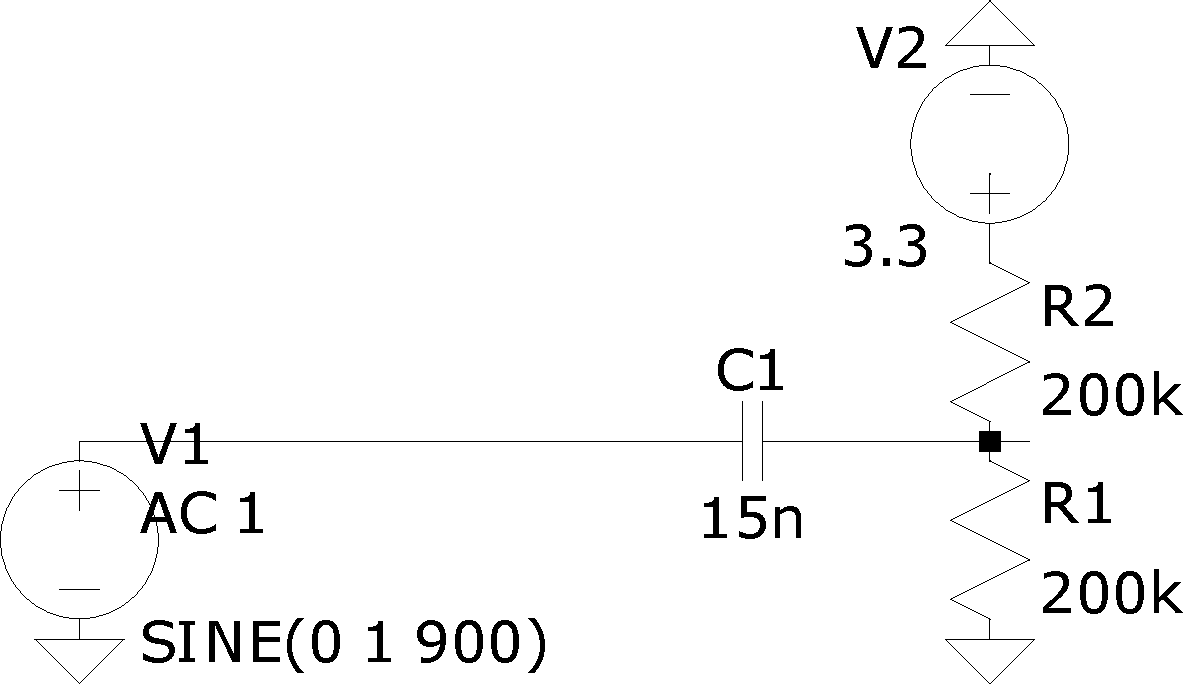
\includegraphics[width=0.3\textwidth]{pdffiles/HighPass/CircuitHighPassPolarization200k.pdf}
    \caption{Schéma de simulation sur LTspice du cas \textit{idéal}}
    \label{fig:ltspice_ideal}
\end{figure}
\begin{figure}[H]
    \centering
    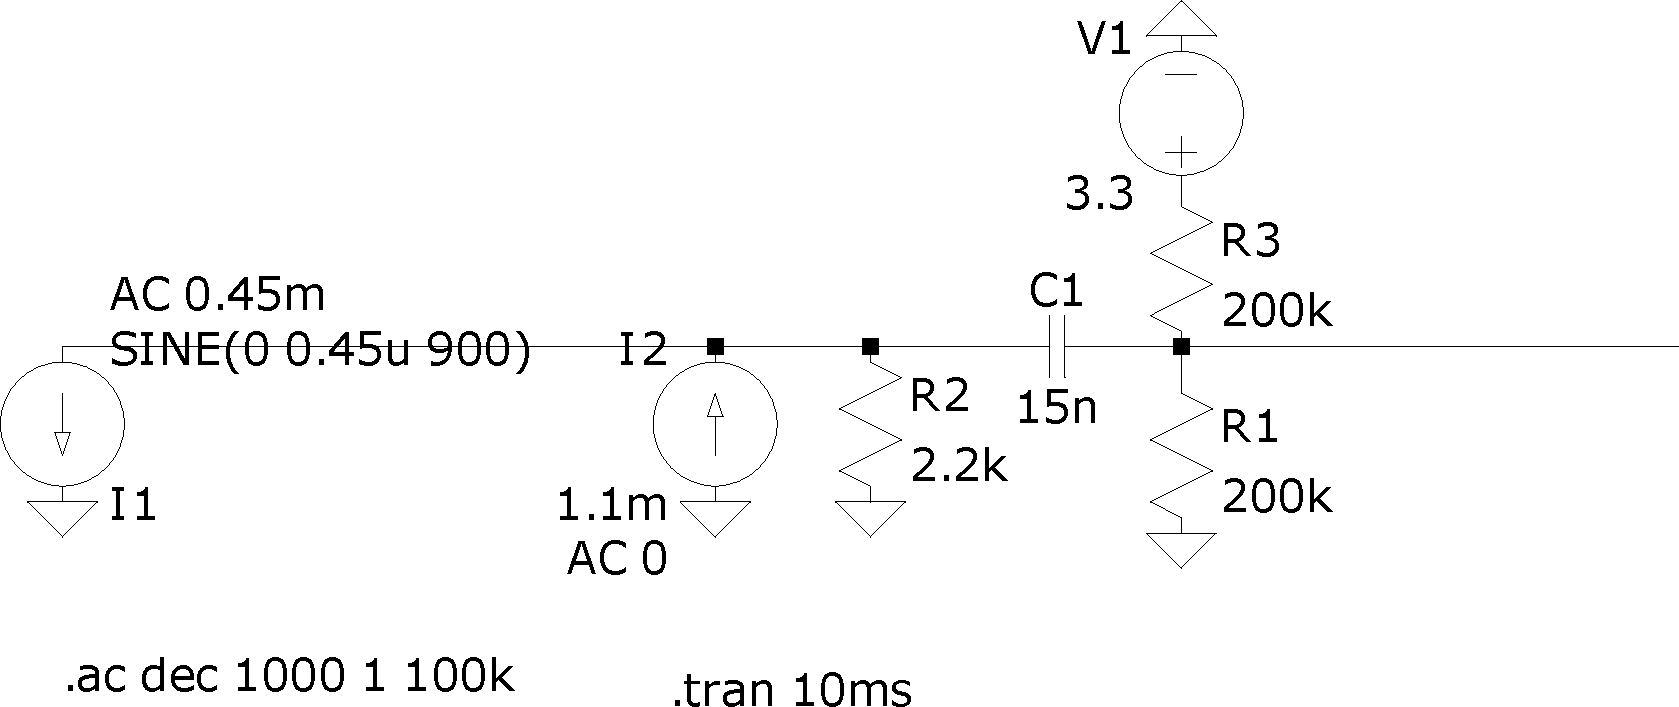
\includegraphics[width=0.4\textwidth]{pdffiles/HighPass/CircuitHighPassSimulationCurrent.pdf}
    \caption{Schéma de simulation sur LTspice du cas \textit{équivalent courant}}
    \label{fig:ltspice_current}
\end{figure}
\begin{figure}[H]
    \centering
    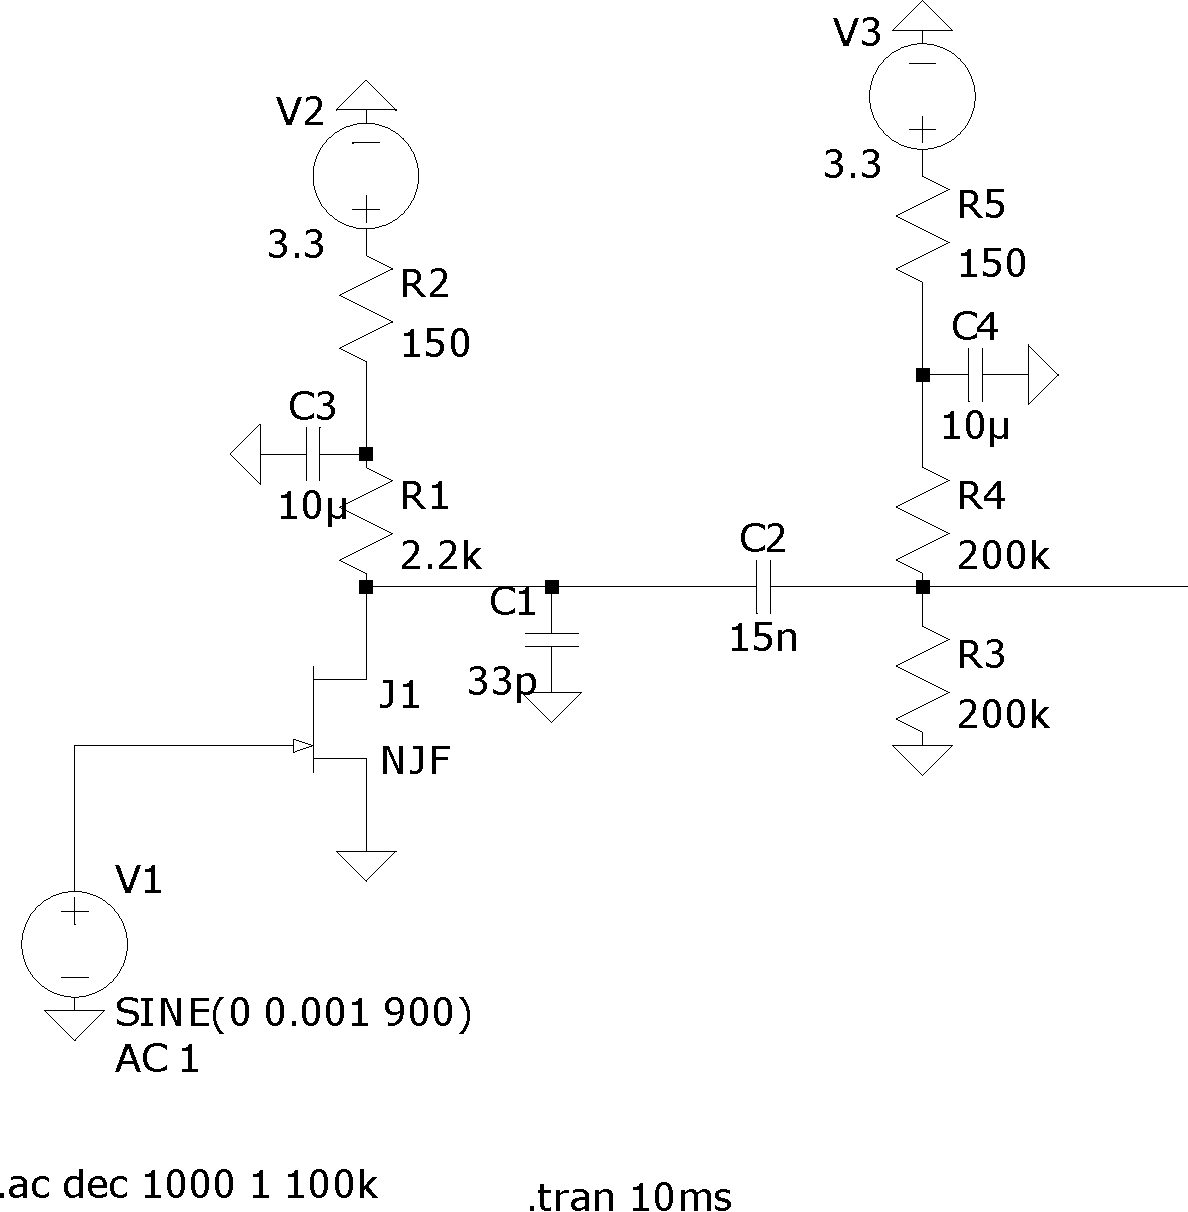
\includegraphics[width=0.4\textwidth]{pdffiles/HighPass/CircuitHighPassSimulationJET.pdf}
    \caption{Schéma de simulation sur LTspice du cas \textit{équivalent transistor}}
    \label{fig:ltspice_transistor}
\end{figure}



Après simulation, on obtient sur la figure \ref{fig:bodesim} les courbes de Bode des différents circuits. On remarque que les courbes ont toutes la même allure, avec une fréquence de coupure située aux alentours de $100 \ Hz$. Par ailleurs, dans la simulation avec transistor, le gain est en dessous de $ 0 \ dB$. Ce n'est pas un problème car ce qui nous intéresse est l'impact de la résistance de polarisation et des filtres passe-bas sur les caractéristiques du filtre passe-haut : \textbf{la fréquence de coupure}.

On en conclut que la résistance de polarisation et les filtres passe-bas ont une influence négligeable sur les caractéristiques du filtre passe-haut.



\begin{figure}[H]
    \centering
    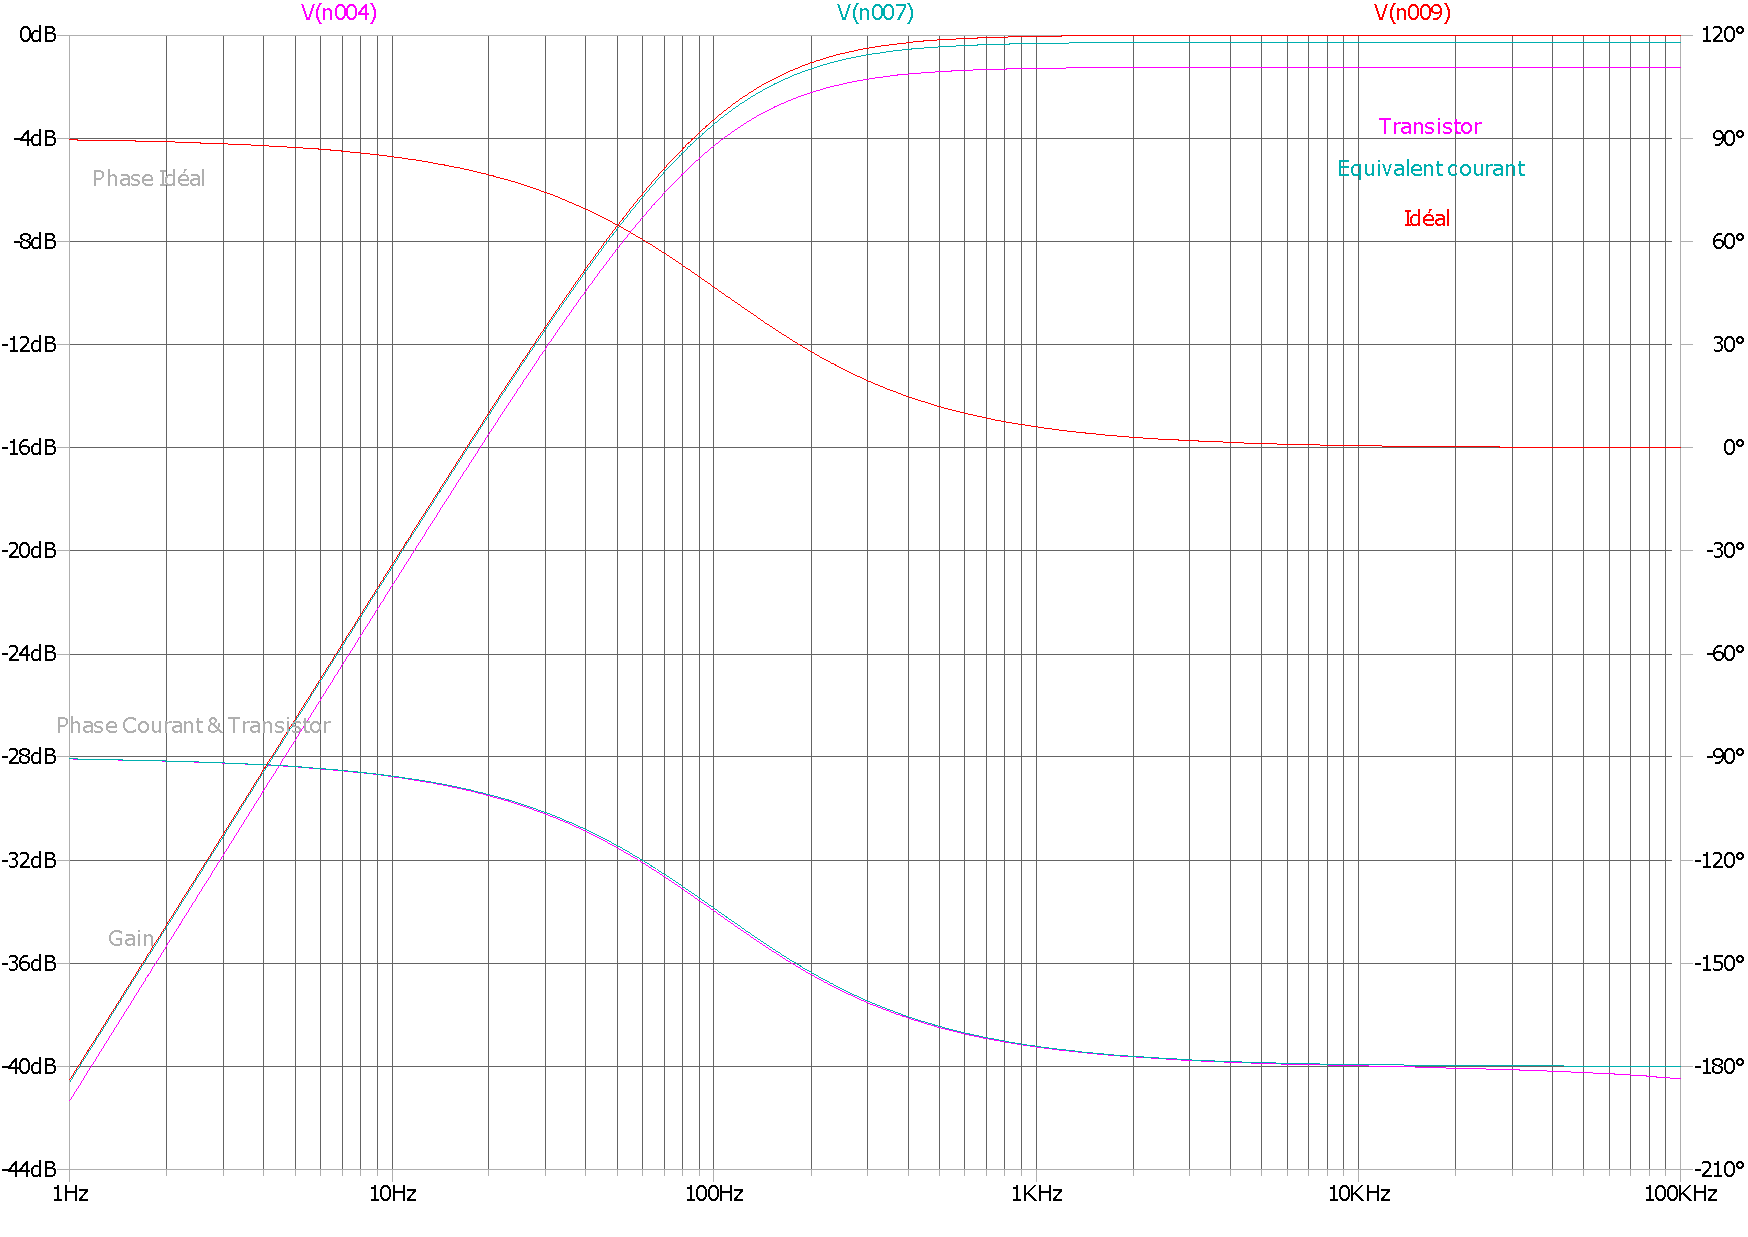
\includegraphics[width=\textwidth]{pdffiles/HighPass/BodeHighPassImpactePolarisation.pdf}
    \caption{Courbe de Bode du filtre passe-haut dans différent cas. Cas \textit{idéal} en rouge, cas \textit{équivalent courant} en bleu et cas \textit{équivalent transistor} en rose }
    \label{fig:bodesim}
\end{figure}

\subsubsection{Critique sur le gain maximal en simulation}

Sachant qu'on ne peut pas obtenir la courbe de Bode de la chaîne d'acquisition à partir du Picoscope, on a décidé de l'obtenir à l'aide de LTspice, en faisant deux simulations. Dans la première, le microphone est remplacé par son équivalent transistor et dans la deuxième par son équivalent source de courant. Pour plus de détails à propos de la simulation et pour voir toutes les courbes, allez voir l'Annexe \ref{Bodechaineacquiannexe}

La figure \ref{fig:BodeFullCircuitJet} est la courbe obtenue dans le premier cas, qui est le pire, et on se rend compte qu'on n'atteint pas le gain voulu. En effet, on peut voir que le gain à $1100 \ Hz$ est de $61.58 \ dB$. Pour rappel, le gain souhaité est de $64.35 \ dB$. 
De manière plus générale, il y aura toujours une différence entre le gain souhaité et le gain réel.

\begin{figure}[H]
    \centering
    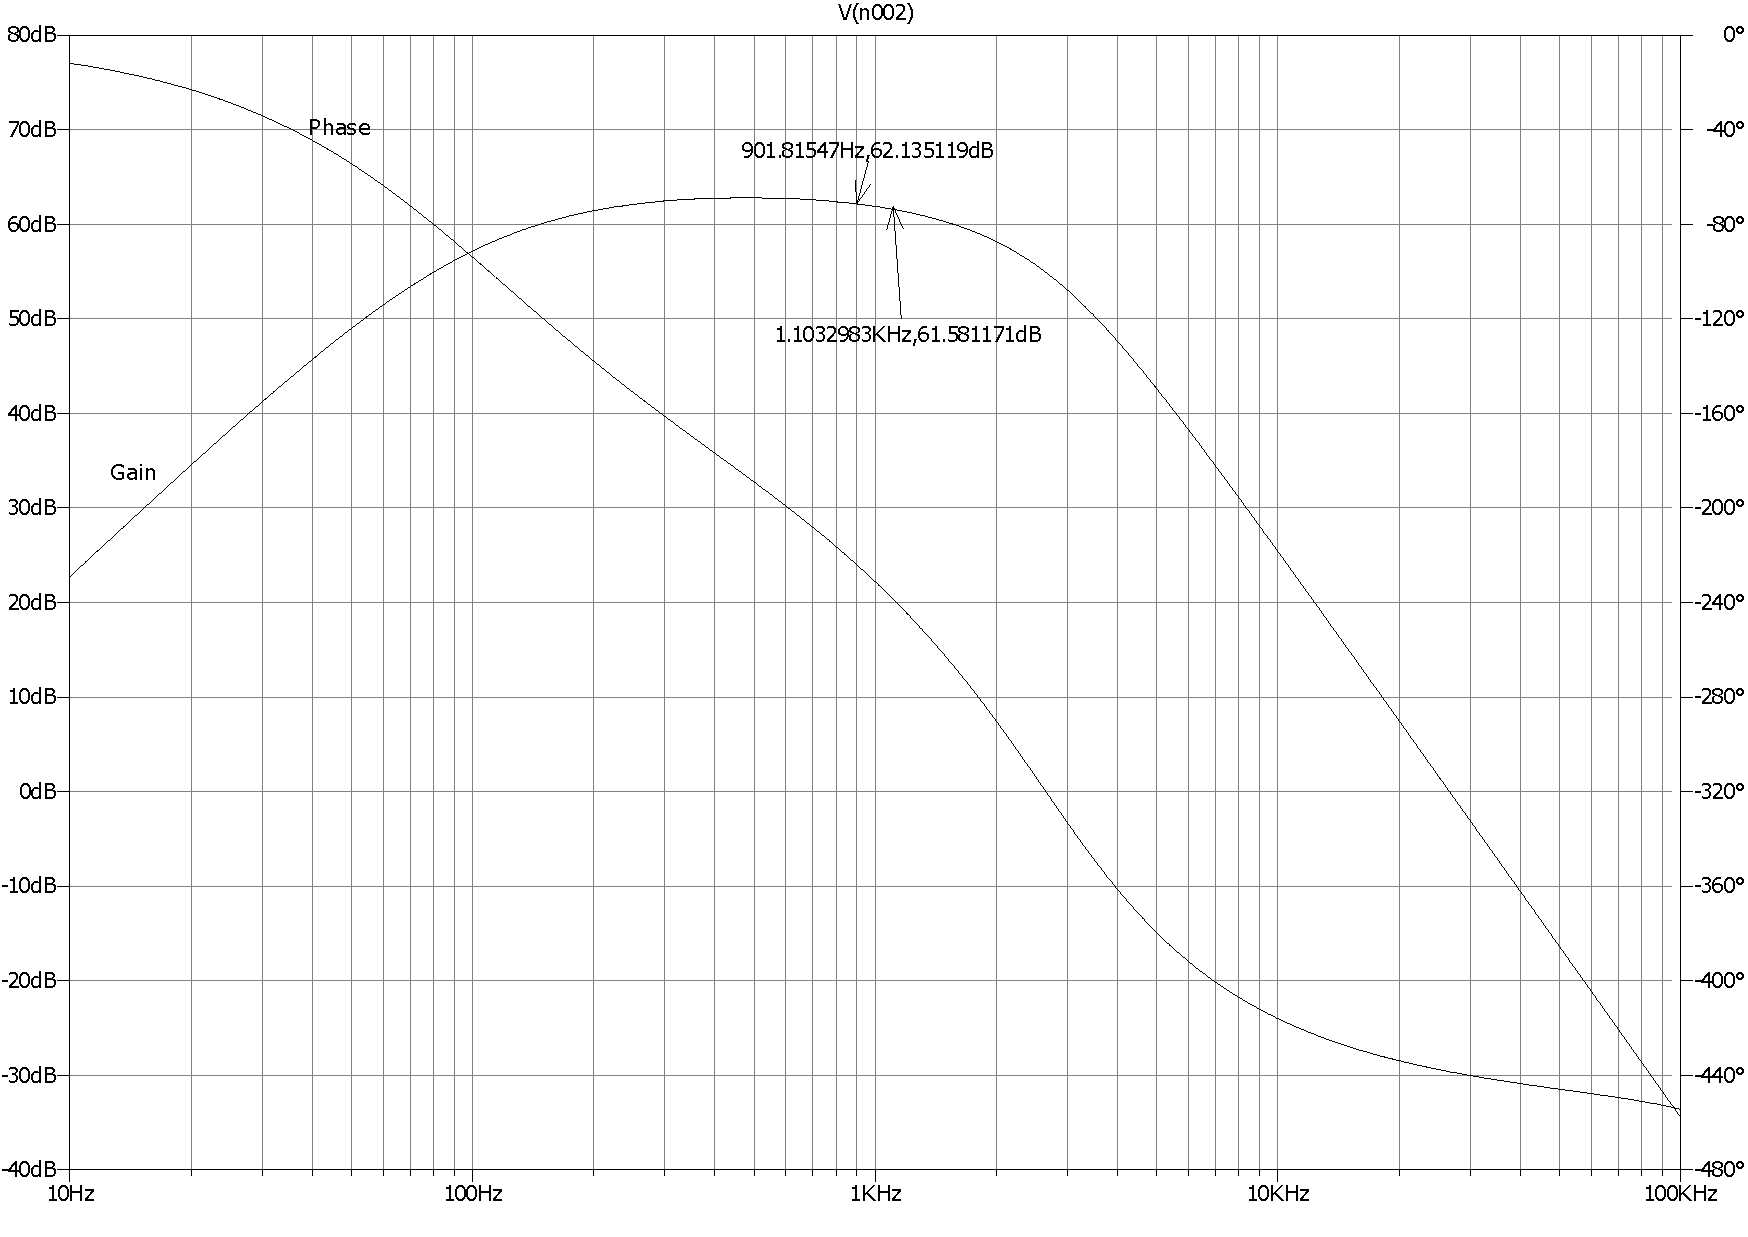
\includegraphics[width=\textwidth]{pdffiles/BodeCircuitJET.pdf}
    \caption{Courbe de Bode de la chaîne d'acquisition. Le microphone est remplacé par son équivalent transistor}
    \label{fig:BodeFullCircuitJet}
\end{figure}

Nous avons décidé de ne rien changer mais on peut toujours rajouter une petite marge en augmentant le gain de l'étage d'amplification. C'est faisable car le gain maximal à $1100 \ Hz$ en un seul étage est de $68.11 \ dB$. Attention cependant à ne pas trop l'augmenter, on veut éviter la saturation.

\newpage


\section{Conversion Analogique-Numérique}

\subsubsection{Configuration}

Une fois que le signal de commande audio sort de la chaîne d'acquisition, il faut le convertir en un signal numérique dans le but de le démoduler, comme le montre la figure \ref{fig:adcbloc}. Cette section va détailler la mise en place de l'ADC.

\begin{figure}[H]
    \centering
    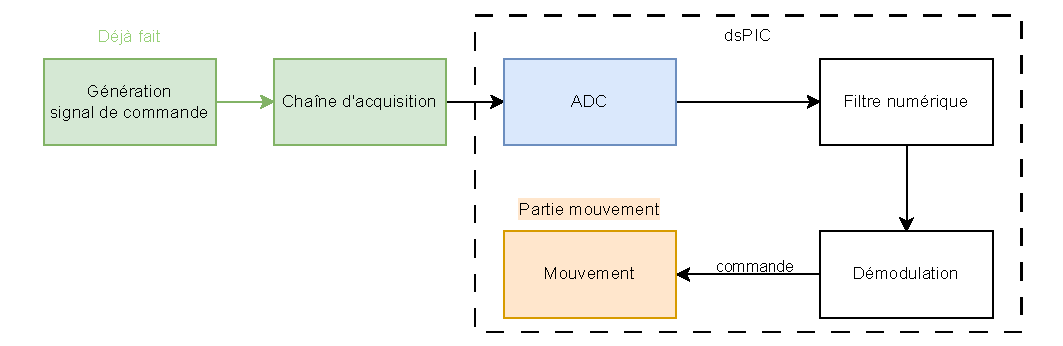
\includegraphics[scale=0.8]{pdffiles/ADCbloc.drawio.pdf}
    \caption{Schéma-bloc de la partie communication, focus sur l'ADC}
    \label{fig:adcbloc}
\end{figure}

Tout d'abord, nous devons configurer le périphérique du dsPIC chargé de la conversion à l'aide d'une librairie. Celle-ci inclut deux modes de fonctionnement :

\begin{itemize}
    \item [$\bullet$] \textit{Manuel} : le déclenchement de la conversion est lancé par le code
    \item [$\bullet$] \textit{Automatique} : le déclenchement de la conversion est lancé par le débordement du \textbf{TIMER3}
\end{itemize}

C'est ce deuxième mode qui sera utilisé car la démodulation est un processus qui doit être rapide et le mode automatique se réalise sans l'intervention du CPU.

Après avoir configuré le périphérique, on doit fixer la période d'échantillonnage de l'ADC en fixant la période de débordement du \textbf{TIMER3}. Mais avant, il faut déterminer cette période d'échantillonnage.

La fréquence d'échantillonnage est choisie telle que les fréquences qui se replient sur les fréquences utiles soient atténuées. Cela revient à choisir, au minimum, 2 fois la fréquence au milieu du segment formé par la fréquence de coupure du filtre de garde et la première fréquence atténuée par le filtre de garde (atténuation à 0.05). Ceci est représenté sur la figure \ref{fig:fs}.  

\begin{figure}[H]
    \centering
    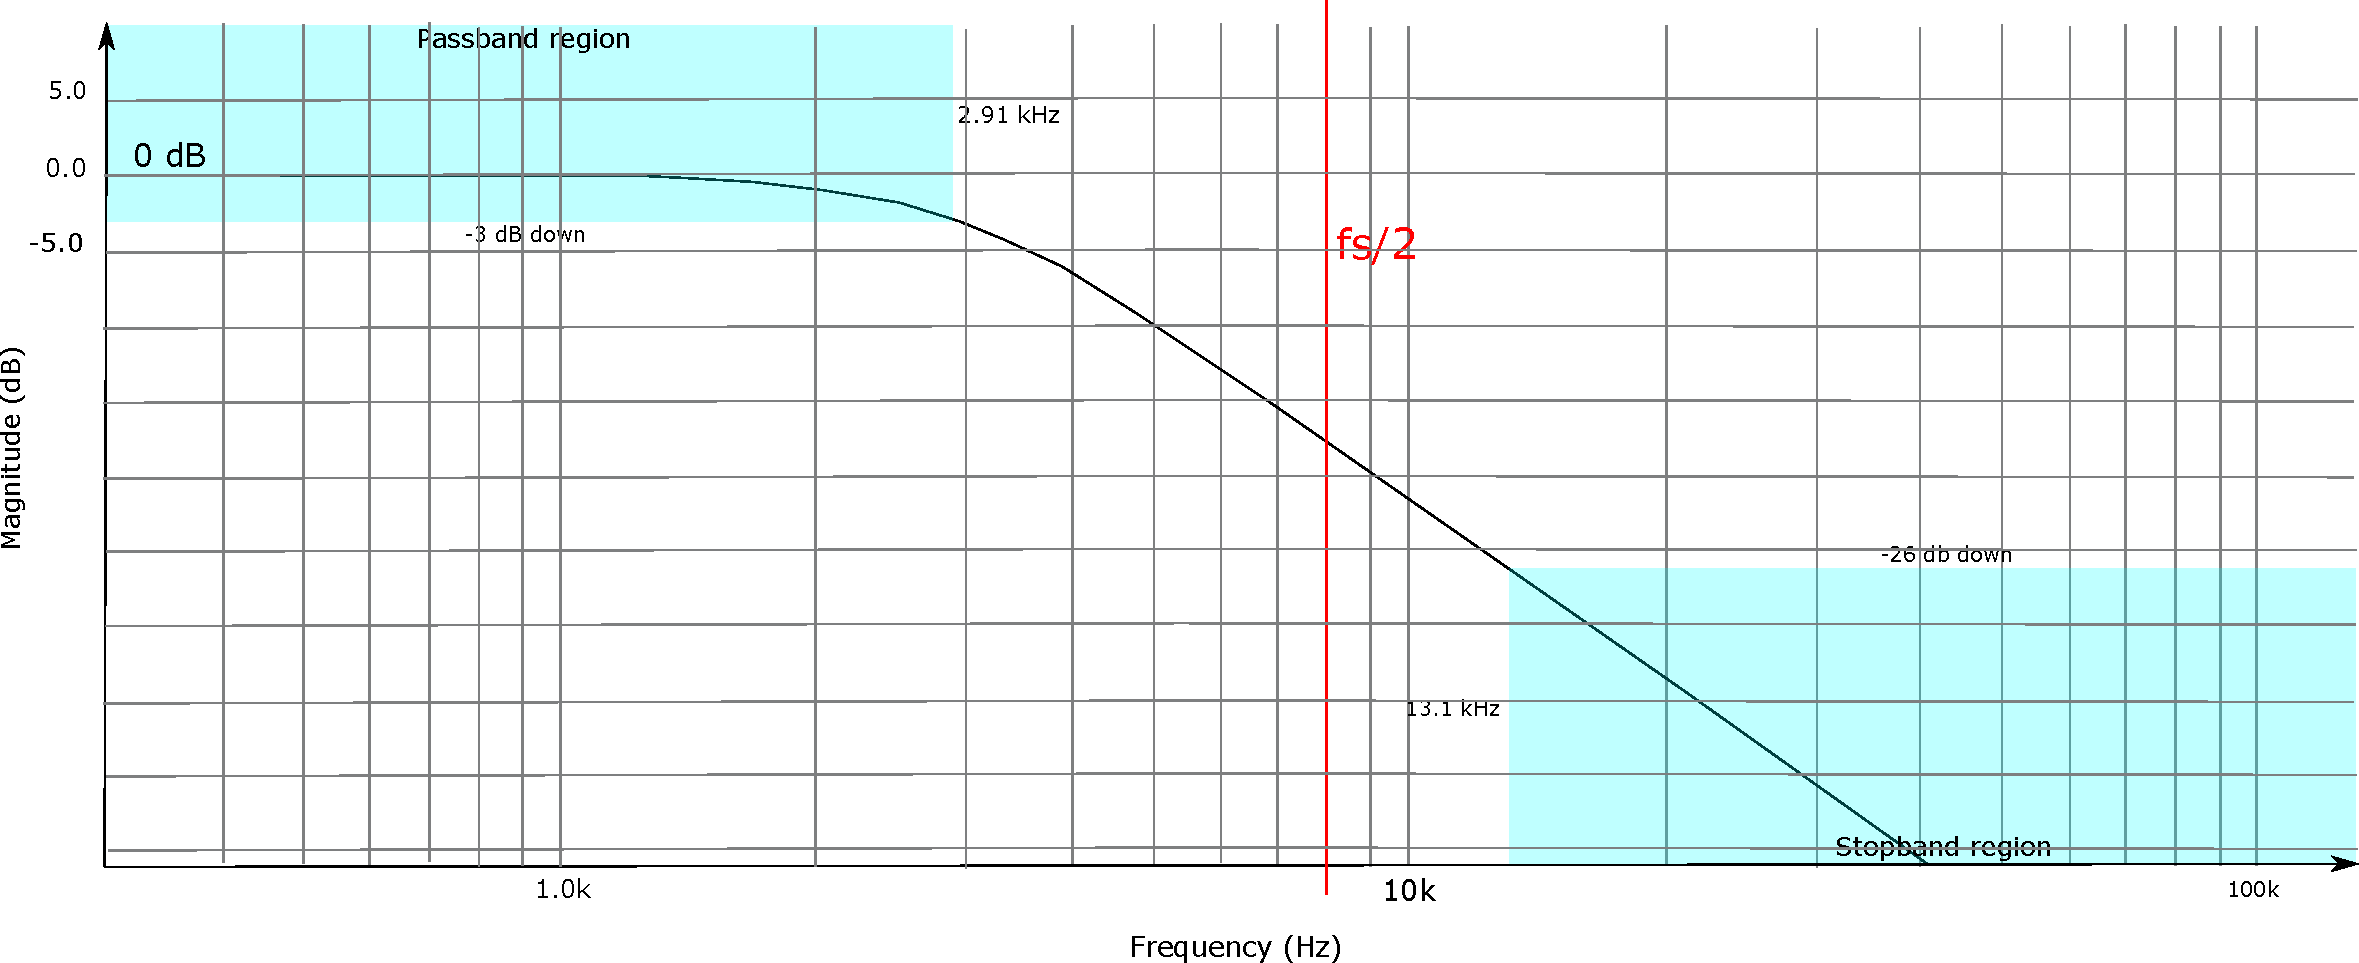
\includegraphics[width=1\textwidth]{pdffiles/lowpassspecINK.pdf}
    \caption{Illustration de la fréquence d'échantillonnage sur la courbe de Bode du filtre de garde}
    \label{fig:fs}
\end{figure}


Autrement dit, la fréquence d'échantillonnage minimale vaut :

\begin{align*}
    f_s &=\left(f_c+ \frac{f_{\text{repliement}}-f_c}{2}\right) \times 2 \\
    &= f_c + f_{\text{repliement}} \\
    &= 2914.050095+13023.87554 \\
    &= 15937.92545 \ Hz
\end{align*}

On peut à présent déterminer la période de débordement à partir de la formule suivante\footnote{On peut remarquer que FCY vaut 40 MHz : on a overclock le dsPIC} :

\begin{align*}
    & PR3 = (FCY \times T_s) - 1 \\
    & \text{Sachant que $FCY$ vaut $40 \ MHz$ et que $\frac{1}{f_s}=62.7434 \ \mu s$,} \\
   \iff & PR3=(40 \ MHz \times 62.7434 \ \mu s) -1 =2508.736 \\
   \hookrightarrow & PR3 \approx 2508 
\end{align*}

On arrondi PR3 à l'entier le plus bas, de cette façon la fréquence d'échantillonnage est plus grande que la fréquence minimale.

Il ne reste plus qu'à implémenter le code dans le dsPIC. On peut tout simplement reprendre le projet adc-dac2.X disponible dans le gitlab du projet et le modifier un peu.

\subsubsection{Validation de l'ADC}

Avant de passer à la démodulation du signal de commande audio, il faut vérifier que l'ADC fonctionne correctement. Pour vérifier que le signal numérique correspond au signal d'entrée, on peut utiliser le projet oscilloscope.X. En effet, en reliant le dsPIC à un PC à l'aide d'un périphérique UART $\leftrightarrow$ USB, on peut observer la forme du signal numérisé. 

Après avoir modifier le nombre de samples et la période d'échantillonnage dans le fichier oscilloscope.py, on peut afficher le résultat de la conversion. Les figures \ref{fig:900HZADC} \& \ref{fig:1100HZADC} nous permettent de valider le bon fonctionnement de l'ADC.



\begin{figure}[H]
    \centering
    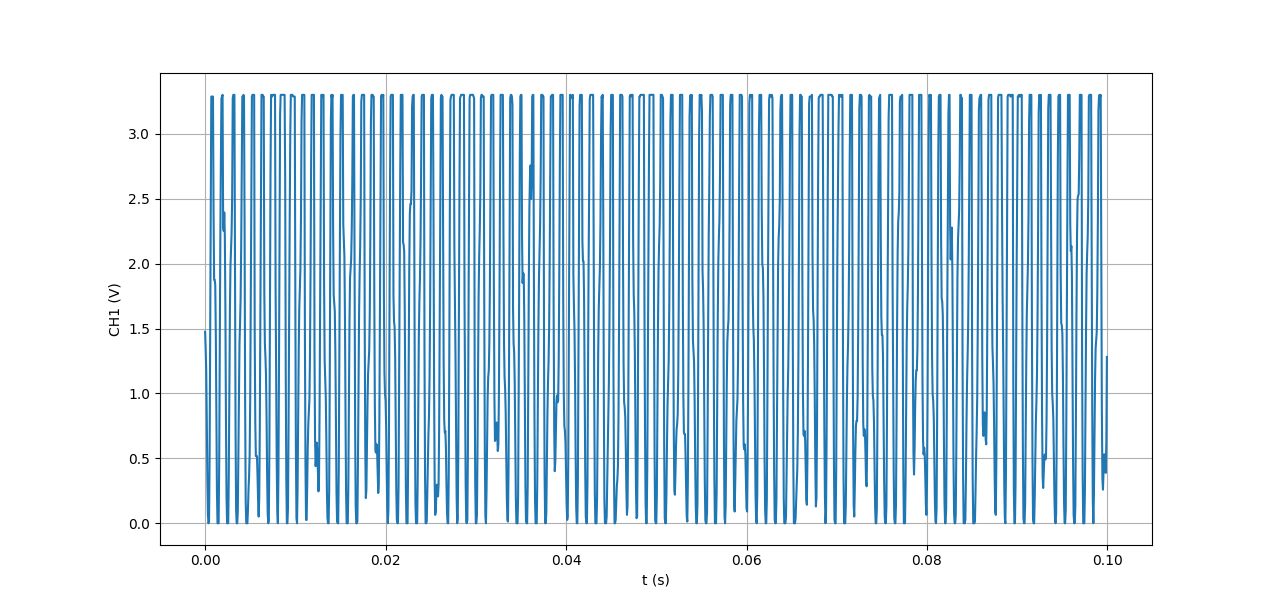
\includegraphics[width=0.7\textwidth]{Pictures/900HZ_ADC.png}
    \caption{Signal numérisé par le dsPIC. Le signal d'entrée est un signal audio de 900 Hz}
    \label{fig:900HZADC}
\end{figure}

\begin{figure}[H]
    \centering
    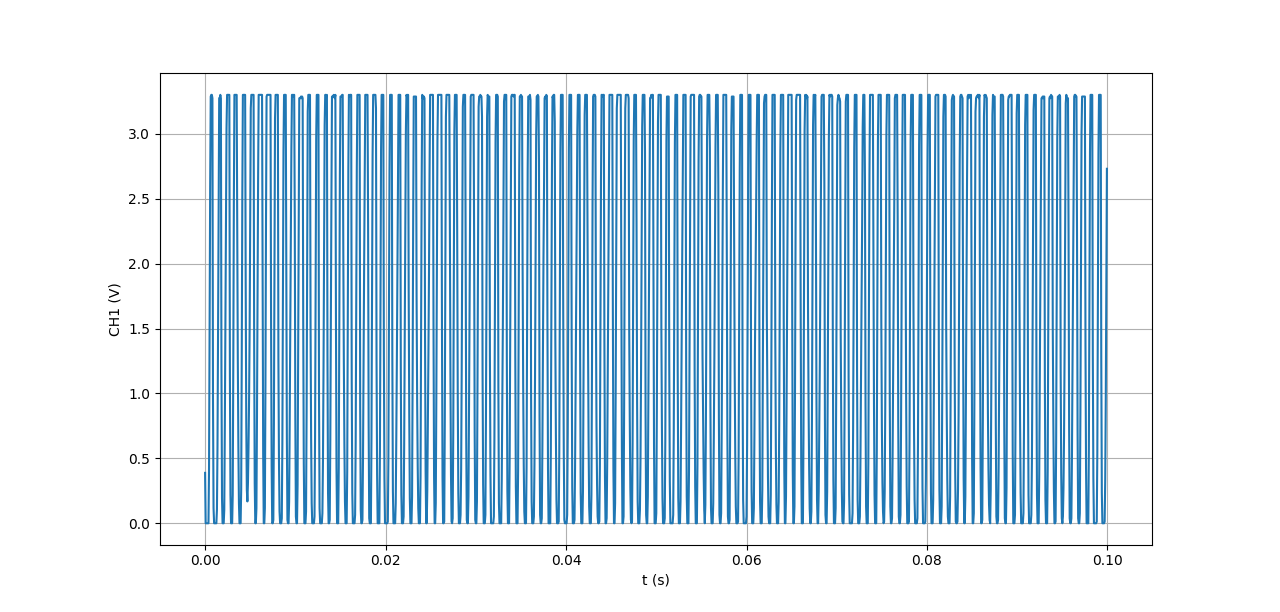
\includegraphics[width=0.7\textwidth]{Pictures/1100HZ_ADC.png}
    \caption{Signal numérisé par le dsPIC. Le signal d'entrée est un signal audio de 1100 Hz}
    \label{fig:1100HZADC}
\end{figure}

\textbf{Remarque} : Il faut modifier la manière dont les données sont envoyés via l'UART. On ne peut pas directement envoyer le résultat d'une conversion via l'UART car le temps que la donnée s'envoie, le \textbf{TIMER3} déborde et on perd de l'information. Il y a deux manières de régler ce problème.

\begin{itemize}
    \item [$\bullet$] Augmenter le débit de la transmission UART
    \item [$\bullet$] Attendre la fin de l'acquisition pour envoyer les résultats à l'ordinateur
\end{itemize}

Nous avons opté pour la deuxième solution dans le cadre de la validation de l'ADC.

\newpage
\section{Filtre numérique}
Une fois le signal numérique reçu par l'ADC, il est important de passer ce signal dans un filtre numérique afin de ne conserver que les informations pertinentes (voir Fig. \ref{fig:filtrenumbloc}). Pour ce faire, nous avons dû faire face à différents choix afin de modéliser le filtre de la manière la plus efficace possible.

\begin{figure}[H]
    \centering
    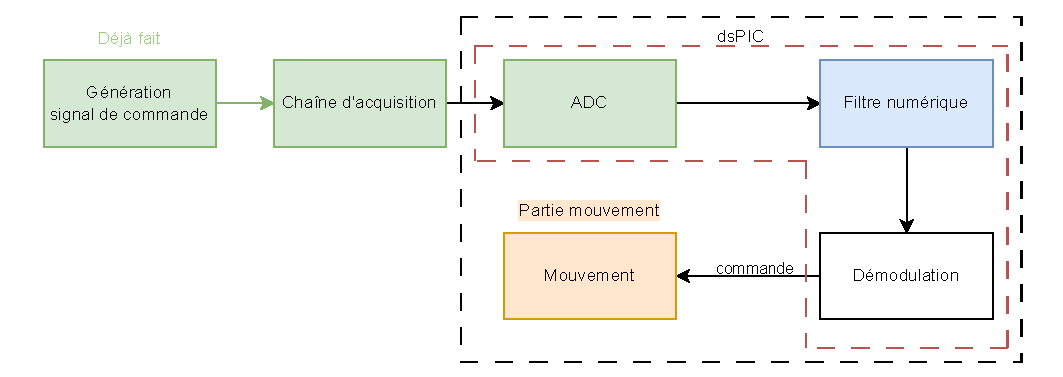
\includegraphics[scale=0.8]{pdffiles/filtrenumbloc.pdf}
    \caption{Schéma-bloc de la partie communication, focalisé sur le filtre numérique. La partie en rouge est détaillée sur la Figure \ref{fig:block_diagram}}
    \label{fig:filtrenumbloc}
\end{figure}

\begin{figure}[h]
    \centering
    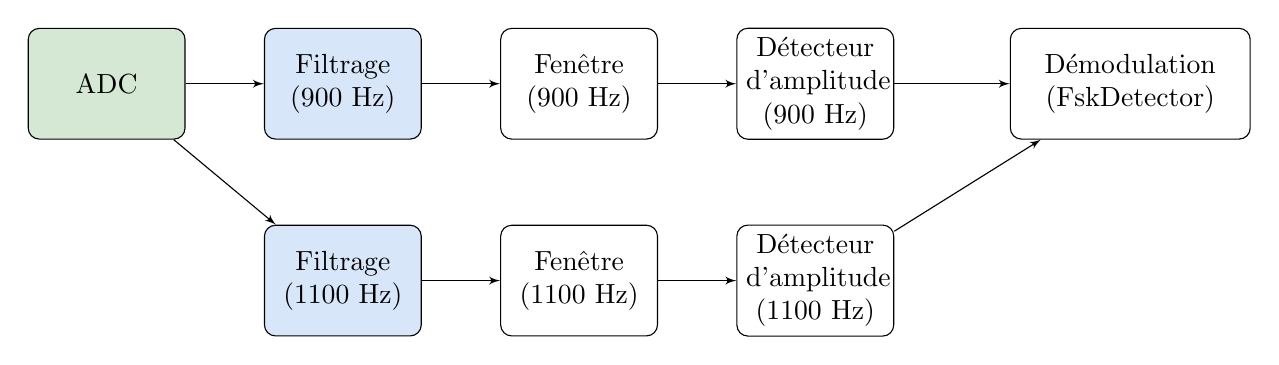
\begin{tikzpicture}[node distance=2cm, auto]
        % ADC Block
        \node [block,fill=mygreen] (adc) {ADC};
        
        % Blocks for 900 Hz
        \node [block, right of=adc, node distance=3cm, fill=myblue] (filter1) {Filtrage (900 Hz)};
        \node [block, right of=filter1, node distance=3cm] (window1) {Fenêtre (900 Hz)};
        \node [block, right of=window1, node distance=3cm] (detector1) {Détecteur d'amplitude (900 Hz)};
        
        % Blocks for 1100 Hz
        \node [block, below of=filter1, node distance=2.5cm, fill=myblue] (filter2) {Filtrage (1100 Hz)};
        \node [block, right of=filter2, node distance=3cm] (window2) {Fenêtre (1100 Hz)};
        \node [block, right of=window2, node distance=3cm] (detector2) {Détecteur d'amplitude (1100 Hz)};
        
        % Demodulation Block
        \node [block, right of=detector1, node distance=4cm, text width=8em] (demod) {Démodulation\\ (FskDetector)};

        % Connecting lines for 900 Hz
        \path [line] (adc) -- (filter1);
        \path [line] (filter1) -- (window1);
        \path [line] (window1) -- (detector1);
        \path [line] (detector1) -- (demod);
        
        % Connecting lines for 1100 Hz
        \path [line] (adc) -- (filter2);
        \path [line] (filter2) -- (window2);
        \path [line] (window2) -- (detector2);
        \path [line] (detector2) -- (demod);
    \end{tikzpicture}
    \caption{Schéma-bloc détaillé entre l'ADC et la Démodulation, focalisé sur le filtre numérique}
    \label{fig:block_diagram}
\end{figure}

\subsection{Filtre FIR ou IIR}

\subsubsection{Filtres FIR}

Les filtres FIR sont caractérisés par une structure qui ne fait pas appel à la rétroaction. Leur sortie est calculée uniquement à partir de leur entrée et ils ont l'équation suivante:
\[
y[n] = \sum_{i=0}^{N} b_i x[n-i]
\]
où $b_i$ sont les coefficients du filtre, $x[n]$ est le signal d'entrée, et $N$ est l'ordre du filtre.

Les principaux avantages des filtres FIR sont leur bonne stabilité et la possibilité de réaliser une réponse en fréquence strictement linéaire. Cependant, pour atteindre des spécifications strictes de la bande de transition et de l'atténuation dans la bande d'arrêt, ils requièrent un ordre très élevé, ce qui est peu pratique dans le cadre de ce projet.

\subsubsection{Filtres IIR}

À l'opposé, les filtres IIR utilisent la rétroaction dans leur structure, ce qui les rend plus efficaces qu'un filtre FIR du même ordre pour obtenir une meilleure atténuation. L'équation générale d'un filtre IIR est:
\[
y[n] =  \sum_{j=0}^{N} b_j x[n-j] - \sum_{i=1}^{N} a_i y[n-i]
\]
où $a_i$ et $b_j$ sont les coefficients du filtre, et $N$ est l'ordre du filtre.

Les filtres IIR peuvent être instables si les pôles sont mal placés, mais une bonne conception permet d'éviter ces problèmes.

\subsubsection{Comparaison et Choix}

\textbf{Complexité computationnelle}

Le principal avantage des filtres IIR sur les FIR est leur faible ordre pour une atténuation donnée dans la bande d'arrêt, ce qui se traduit par moins de coefficients et donc moins d'opérations arithmétiques par échantillon traité. Ceci est particulièrement bénéfique dans les applications embarquées où la puissance de calcul et la mémoire sont limitées.

\textbf{Performance en Temps Réel}

La structure récursive des filtres IIR permet une implémentation plus efficace sur des processeurs simples, tels que le dsPIC utilisé pour le robot. Cette efficacité est très importante pour assurer une démodulation rapide et sans perte d'informations.

Le choix entre FIR et IIR dépend aussi des spécificités du système, notamment la tolérance aux phases non-linéaires et la nécessité d'une stabilité absolue. Pour notre robot, la légère phase non-linéaire introduite par un filtre IIR est un compromis acceptable pour bénéficier de sa faible complexité et de sa haute efficacité. Nous avons donc décidé de faire un filtre numérique IIR.

\subsection{Design du filtre numérique}
Pour concevoir les différents étages du filtre numérique, le code Python mis à notre disposition dans le cadre du projet est \textit{digitalFilterDesign.py}. Les filtres passe-bande ont été conçus selon les spécifications suivantes pour chaque fréquence centrale.

\subsubsection{Filtre Passe-Bande à 900 Hz}
\begin{itemize}
\item Fréquence d'échantillonnage : 16000 Hz
\item Fréquence centrale : 900 Hz
\item Largeur de la bande passante : 27 Hz
\item Gain minimum dans la bande passante : 0.9
\item Largeur de la bande bloquante : 63 Hz
\item Gain maximum dans la bande bloquante : 0.1
\end{itemize}

Les coefficients des étages du filtre sont les suivants :
\begin{align*}
    H_1(z) &= 0.001771 \frac{1+2z^{-1}+z^{-2}}{1-1.86370006z^{-1}+0.98824962z^{-2}} \\
    H_2(z) &= 0.001726 \frac{1+2z^{-1}+z^{-2}}{1-1.86719114z^{-1}+0.98840267z^{-2}} \\
    H_3(z) &= 0.023 \frac{1-2z^{-1}+z^{-2}}{1-1.86766577z^{-1}+0.99507105z^{-2}} \\
    H_4(z) &= 0.02283 \frac{1-2z^{-1}+z^{-2}}{1 -1.87591938z^{-1}+ 0.99522511z^{-2}}
\end{align*}
Le gain maximum des étages est 1.6757.

\begin{figure}[H]
    \centering
    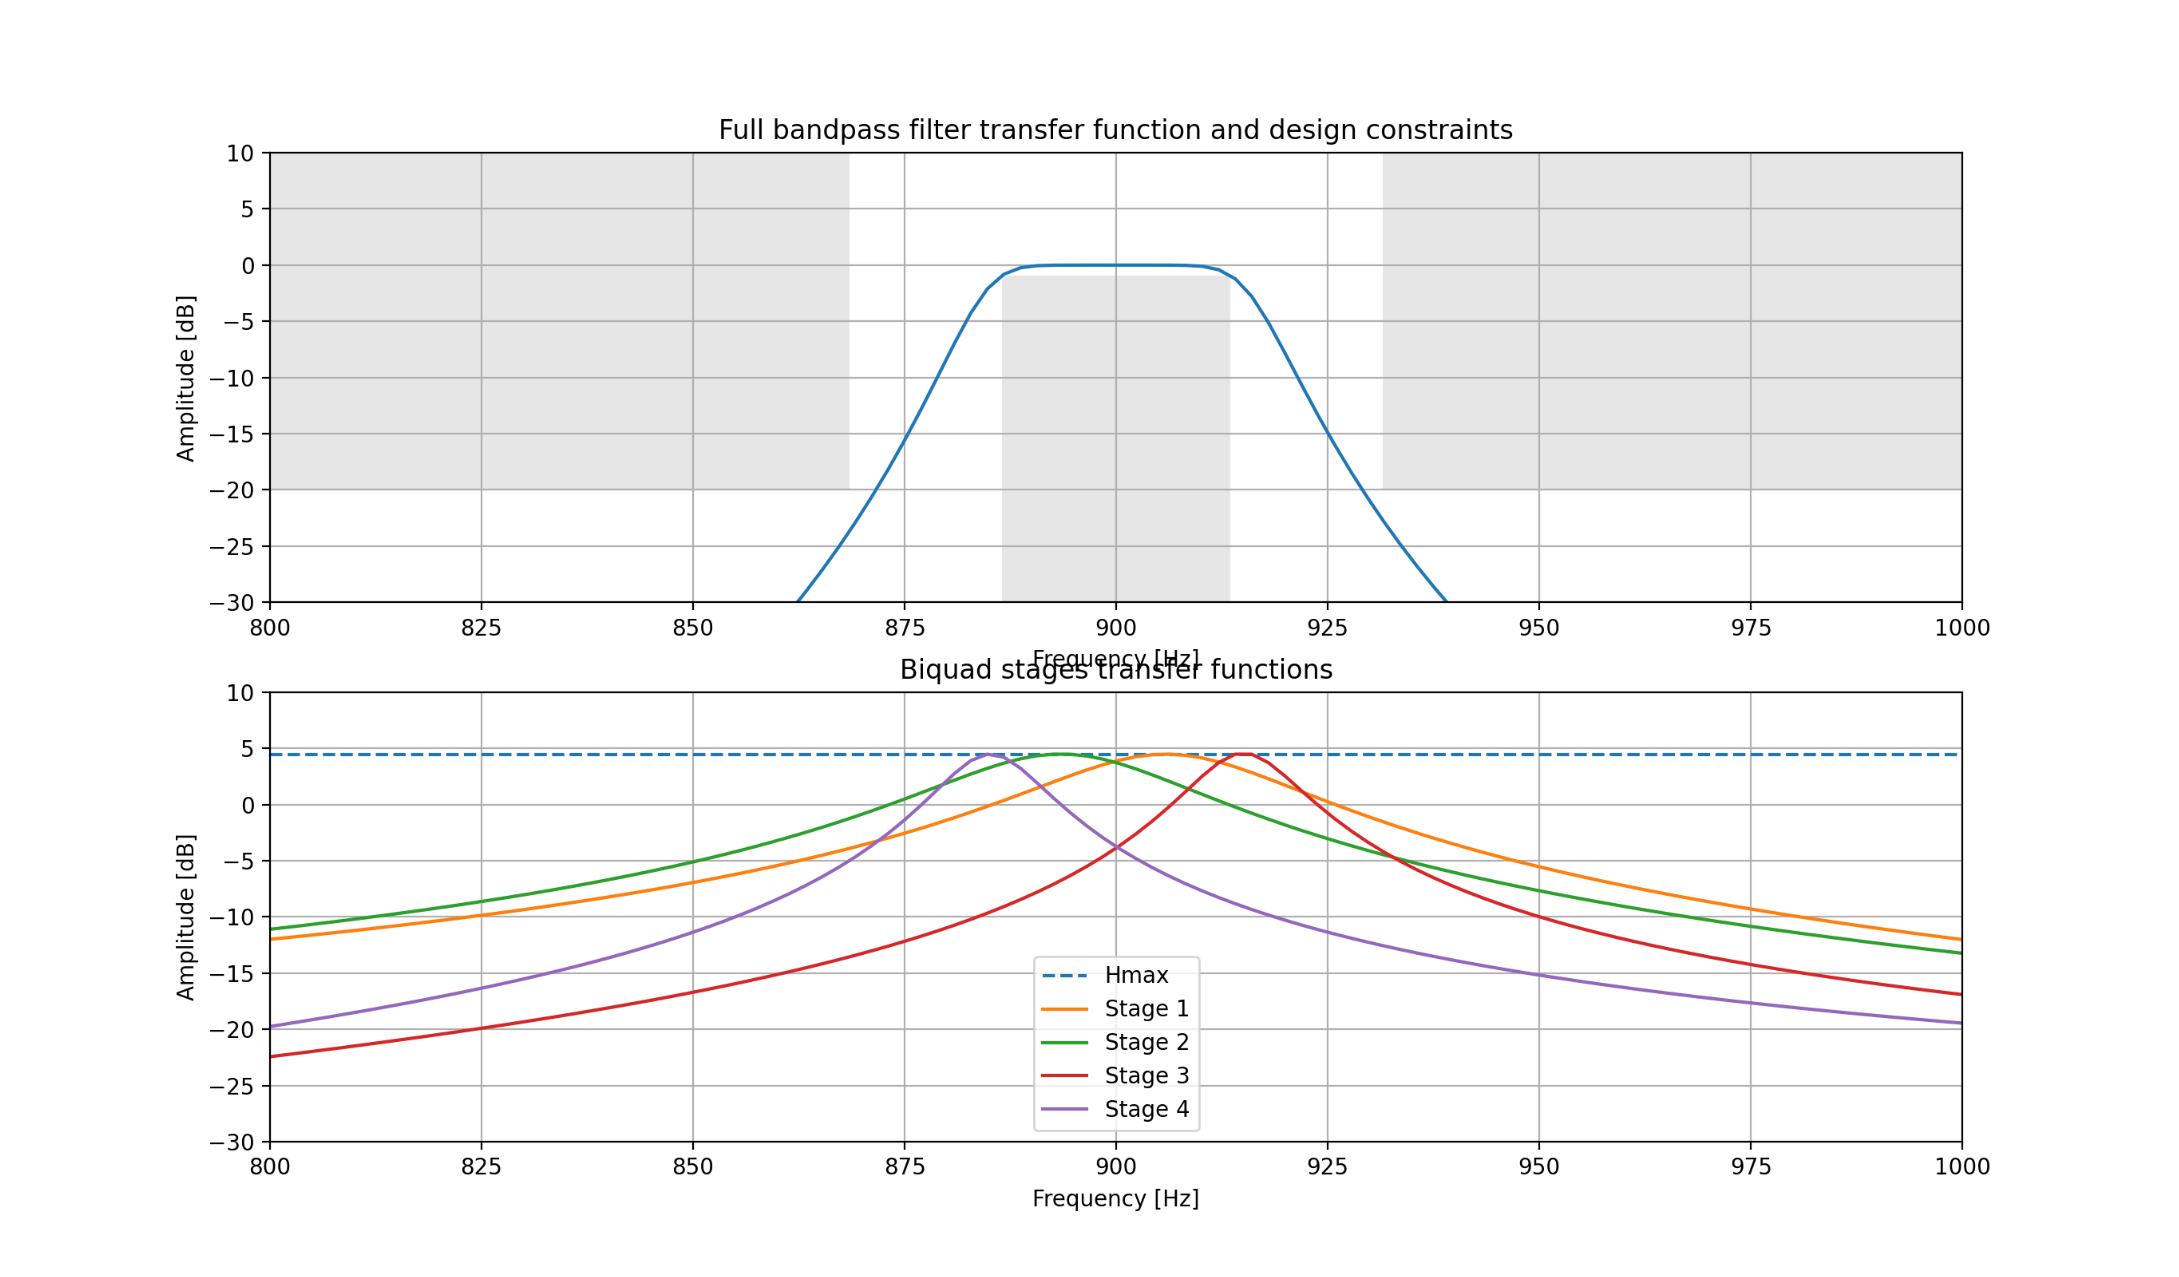
\includegraphics[width=0.7\textwidth]{Pictures/filtre iir 900.png}
    \caption{Filtre passe bande et des différents étages pour la fréquence centrale à 900Hz}
    \label{fig:enter-label}
\end{figure}

\subsubsection{Filtre Passe-Bande à 1100 Hz}
\begin{itemize}
    \item Fréquence d'échantillonnage: 16000 Hz
    \item Fréquence centrale: 1100 Hz
    \item Largeur de la bande passante: 33 Hz
    \item Gain minimum dans la bande passante: 0.9
    \item Largeur de la bande bloquante: 77 Hz
    \item Gain maximum dans la bande bloquante: 0.1
\end{itemize}

Les coefficients des étages du filtre sont les suivants:
\begin{align*}
    H_1(z) &= 0.00259 \frac{1+2z^{-1}+z^{-2}}{1-1.80592184z^{-1}+0.98584165z^{-2}} \\
    H_2(z) &= 0.002661 \frac{1+2z^{-1}+z^{-2}}{1-1.80081358z^{-1}+0.98565917z^{-2}} \\
    H_3(z) &= 0.02277 \frac{1-2z^{-1}+z^{-2}}{1-1.8047745z^{-1}+0.99398116z^{-2}} \\
    H_4(z) &= 0.02273 \frac{1-2z^{-1}+z^{-2}}{1-1.8169234z^{-1}+0.99416513z^{-2}}
\end{align*}
Le gain maximum des étages est 1.6796.
\begin{figure}[H]
    \centering
    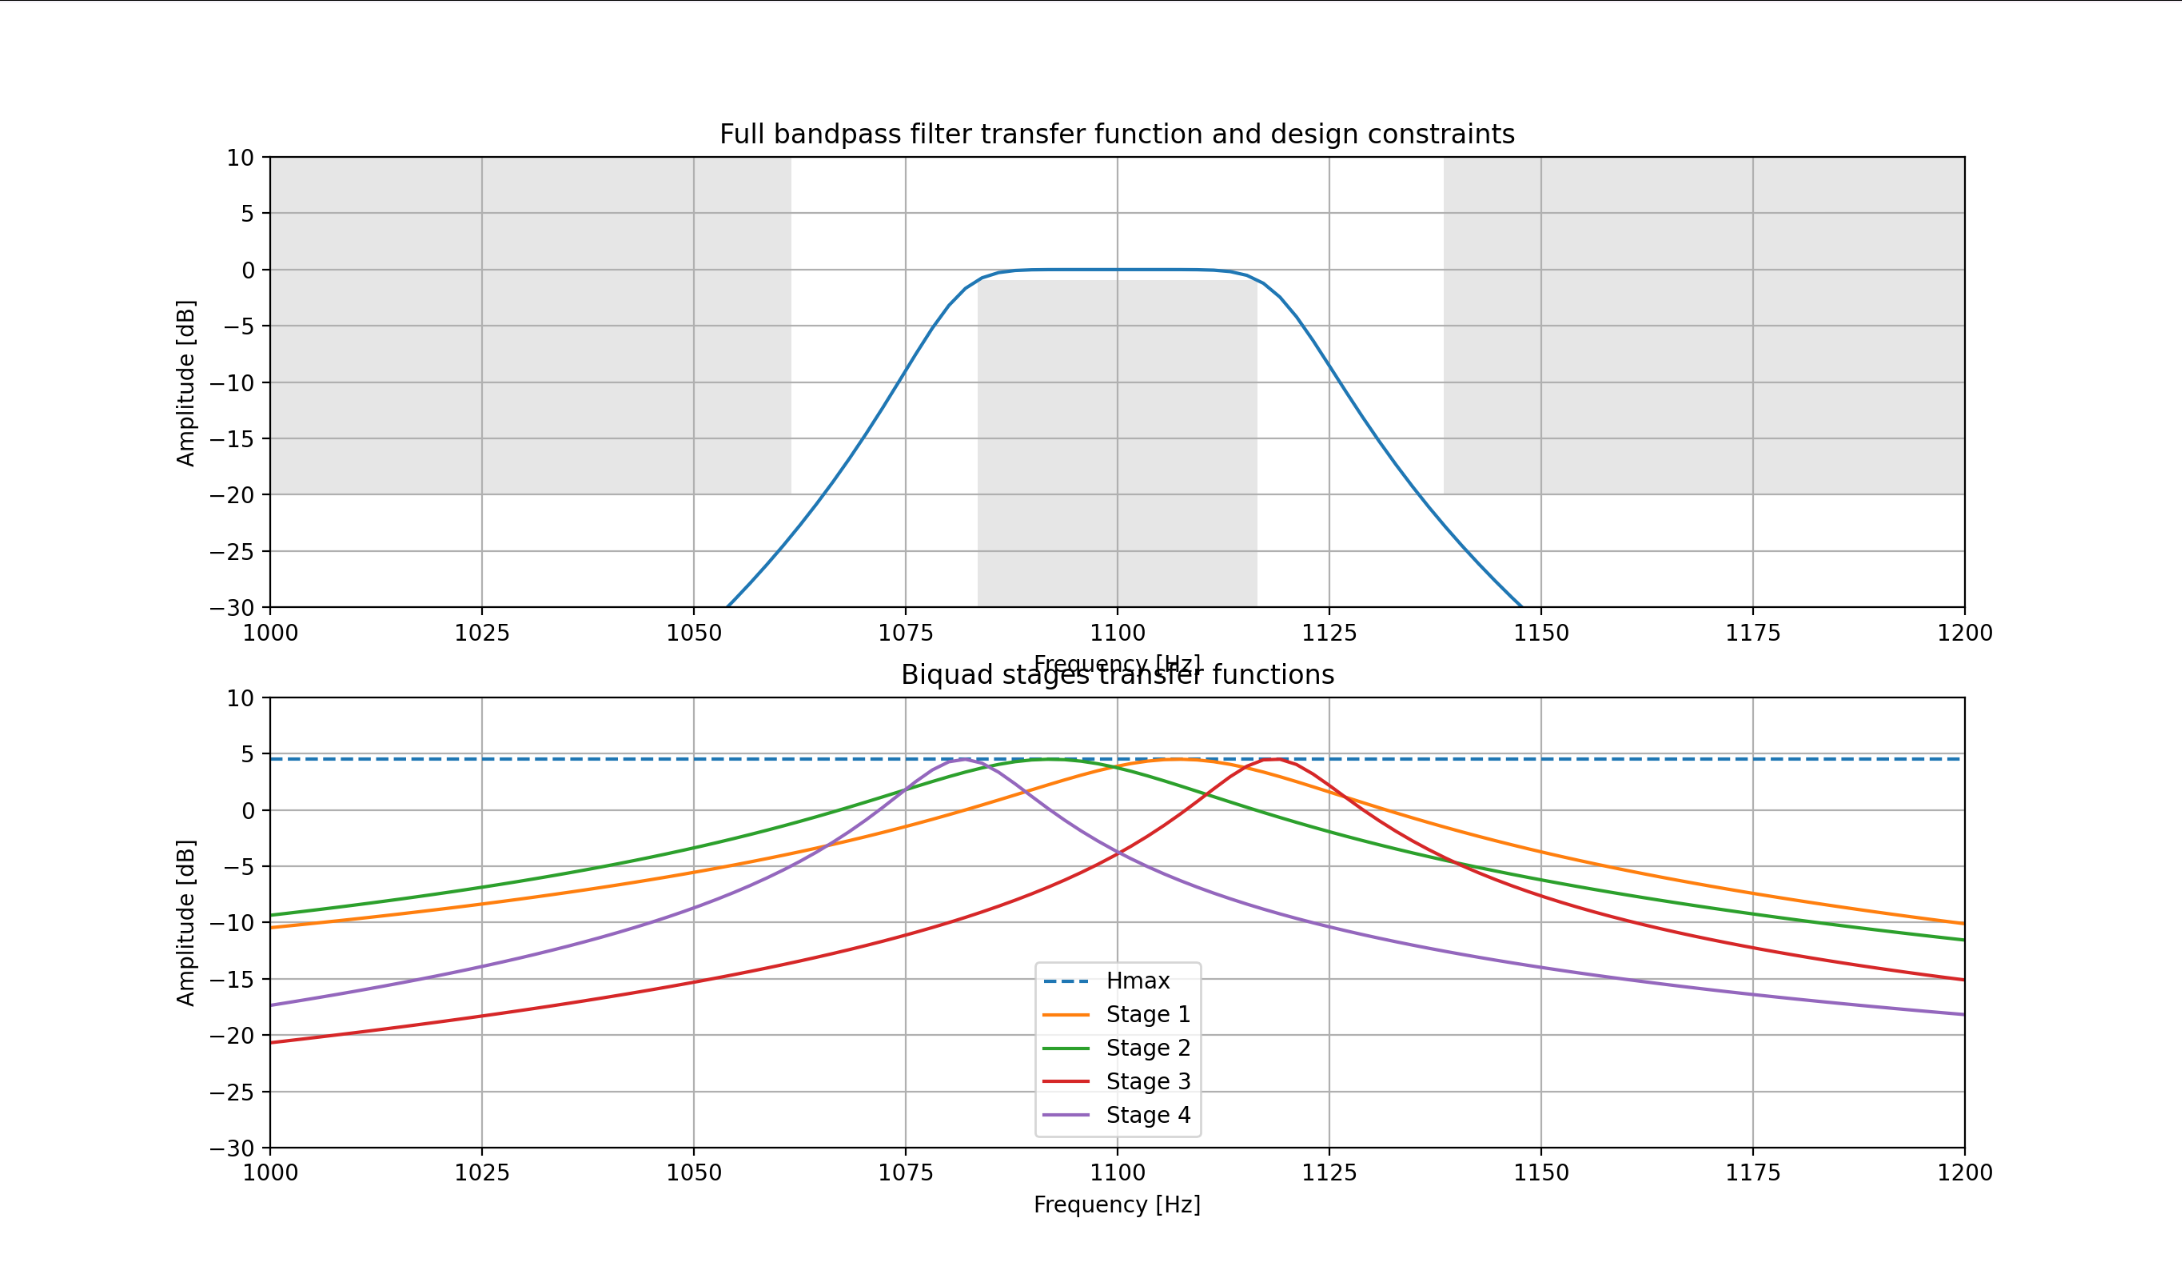
\includegraphics[width=0.7\textwidth]{Pictures/filtre iir 1100.png}
    \caption{Filtre passe bande et des différents étages pour la fréquence centrale à 1100Hz}
    \label{fig:enter-label}
\end{figure}



\input{Filtre num/Implémentation}
\section{Fenêtre Glissante et Seuil d'Amplitude}
\begin{figure}[h]
    \centering
    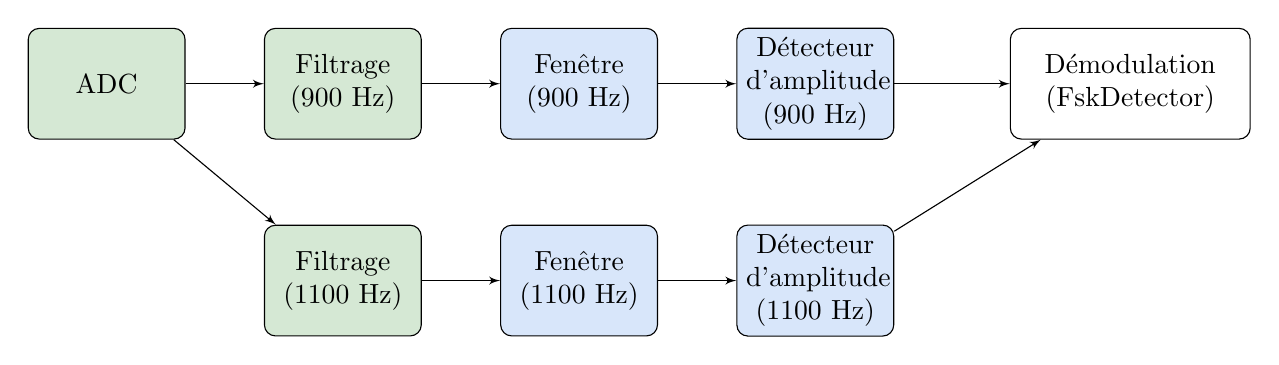
\begin{tikzpicture}[node distance=2cm, auto]
        % ADC Block
        \node [block,fill=mygreen] (adc) {ADC};
        
        % Blocks for 900 Hz
        \node [block, right of=adc, node distance=3cm, fill=mygreen] (filter1) {Filtrage (900 Hz)};
        \node [block, right of=filter1, node distance=3cm,fill=myblue] (window1) {Fenêtre (900 Hz)};
        \node [block, right of=window1, node distance=3cm,fill=myblue] (detector1) {Détecteur d'amplitude (900 Hz)};
        
        % Blocks for 1100 Hz
        \node [block, below of=filter1, node distance=2.5cm,fill=mygreen] (filter2) {Filtrage (1100 Hz)};
        \node [block, right of=filter2, node distance=3cm,fill=myblue] (window2) {Fenêtre (1100 Hz)};
        \node [block, right of=window2, node distance=3cm,fill=myblue] (detector2) {Détecteur d'amplitude (1100 Hz)};
        
        % Demodulation Block
        \node [block, right of=detector1, node distance=4cm, text width=8em] (demod) {Démodulation\\ (FskDetector)};

        % Connecting lines for 900 Hz
        \path [line] (adc) -- (filter1);
        \path [line] (filter1) -- (window1);
        \path [line] (window1) -- (detector1);
        \path [line] (detector1) -- (demod);
        
        % Connecting lines for 1100 Hz
        \path [line] (adc) -- (filter2);
        \path [line] (filter2) -- (window2);
        \path [line] (window2) -- (detector2);
        \path [line] (detector2) -- (demod);
    \end{tikzpicture}
    \caption{Schéma-bloc détaillé entre l'ADC et la Démodulation, focus sur la fenêtre et la détection d'amplitude}
    \label{fig:block_diagram_fe}
\end{figure}
\subsection{Fenêtre Glissante}
\label{fenetre_glissante}
Pour implémenter la démodulation du signal, nous avons implémenter une fenêtre glissante permettant de choisir la plus grande valeur parmi les échantillons dans la fenêtre. La fréquence d'échantillonnage étant de 16 kHz, il a fallu faire une fenêtre glissante sur $\frac{16000 \text{ Hz}}{900 \text{ Hz}} \approx 17$ échantillons et sur $\frac{16000 \text{ Hz}}{1100 \text{ Hz}} \approx 15$ échantillons. Il est acceptable de considérer une fenêtre glissante identique pour les deux fréquences prenant en compte 16 échantillons. Il est important de considérer que désormais, à la sortie de ce bloc, nous ne travaillons plus à 16 kHz mais bien à 1 kHz, étant donné que la fenêtre glissante ne renvoie que le plus grand échantillon parmi 16. 

\subsubsection{Implementation de la Fenêtre Glissante}
Une fois que les échantillons ont été filtrés, un maximum est déterminé dans une fenêtre glissante de 16 échantillons. Pour chaque échantillon traité, s'il s'agit du premier échantillon de la fenêtre, il est initialisé comme maximum. Pour les échantillons suivants, une comparaison est faite pour déterminer si l'échantillon filtré courant est supérieur au maximum actuel. Si c'est le cas, il devient le nouveau maximum.
\subsection{Seuil d'Amplitude}
Le plus grand échantillon à la sortie de la fenêtre glissante est ensuite comparé à un seuil d'amplitude. Ce seuil est choisi en fonction des valeurs des filtres obtenues lors de la simulation du filtre numérique. Pour rappel, les amplitudes maximales obtenues en virgule flottante sur les graphes pour 900 Hz et 1100 Hz étaient respectivement de 3 et 0.75 (\ref{res_filtre_num}).

Dans le code, la sortie du filtre est en virgule fixe. Par conséquent, des seuils de 500 et de 150 ont été choisis pour les amplitudes à 900 Hz et 1100 Hz respectivement. Ces valeurs ont été déterminées à partir de différents tests visant à ajuster précisément les seuils. L'objectif était de trouver un équilibre entre des seuils suffisamment élevés pour éviter que le bruit ne soit interprété comme un signal, mais pas trop élevés afin de ne pas manquer les véritables signaux. Ainsi, les seuils de 500 pour 900 Hz et de 150 pour 1100 Hz garantissent une détection fiable et précise des signaux. La fonction du seuil d'amplitude renvoie 0 si l'amplitude est inférieur au seuil et 1 pour le cas inverse.




\input{Filtre num/Démodulation}
\section{Conclusion du traitement des signaux audio}

Les sections 3.1 à 3.5 de notre projet montrent l'importance d'un traitement du signal  pour assurer le bon fonctionnement de notre robot. Nous avons dimensionné une chaîne d'acquisition qui remplit le cahier des charges. Ensuite, la conversion analogique-numérique (ADC) a été configurée pour permettre une démodulation rapide sans surcharger le CPU. En choisissant des filtres IIR, nous avons pu obtenir une atténuation efficace avec un ordre minimal, facilitant une implémentation rapide et précise. L'utilisation d'une fenêtre glissante de 16 échantillons pour sélectionner le maximum a permis de réduire la fréquence d'échantillonnage effective, tandis que les seuils d'amplitude ajustés empêchent les faux positifs tout en assurant la détection correcte des signaux. La fonction \texttt{fskDetector} analyse les bits 1 ou 0 des deux fréquences centrales à la sortie du seuil d'amplitude pour déterminer l'état du signal et créer une trame de bits, ce qui permet au robot de savoir quelle action exécuter. Il a fallu que toutes ces étapes soient réalisées en moins de 62.5 $\mu$s pour s'assurer de ne pas perdre des informations du signal.



%\section{Démodulation} \label{test}

\newpage
\chapter{Assemblage final}

Nous avons divisé ce projet en deux grandes parties : une partie \textbf{mouvement} et une partie \textbf{traitement des signaux audio}. Pour pouvoir clôturer ce projet, il faut réunir les deux parties.

Comme dit précédemment, on n'utilise qu'un seul dsPIC pour tout le projet. Ainsi, la commande que doit exécuter la partie \textbf{mouvement} est simplement passée en argument lors de l'appel à la fonction concernée. Cet appel se fait à la fin de la partie \textbf{traitement des signaux audio}, lorsque le signal audio a été démodulé. Le code final se trouve dans l'annexe \ref{code:main}.

La dernière étape avant de conclure le projet est de vérifier que le robot fonctionne.

\subsubsection{Critique}

Il faut émettre le signal audio très proche du robot pour qu'il puisse détecter la commande. Ce n'est pas pratique. On peut régler ce problème en trouvant une manière de concentrer le signal dans une direction (changer le microphone et/ou l'émetteur du signal audio).

\newpage
\chapter{Conclusion}

En conclusion, lors de ce projet, nous avons dimensionné une chaîne d'acquisition, nous avons configuré un microcontrôleur (UART, PIO, ADC, TIMER, etc...) et nous avons réalisé un filtre numérique ainsi qu'un régulateur numérique. De plus, ce projet nous a permis de développer une méthode de travail : nous divisons le projet en petit blocs, on travaille sur chaque bloc et on le valide avant de passer au suivant.\\
Après avoir mis en place toutes ces étapes, le robot exécute correctement les instructions du signal audio. L'objectif a donc été atteint à moins de 5\% de translation. 

%\section{Envoie au dsPIC}

\appendix

%Les pages suivantes proviennent du fichier \textit{Analyse du projet.md} disponible dans le \href{https://gitlab.com/mosee/elech309-2024}{gitlab du projet}
%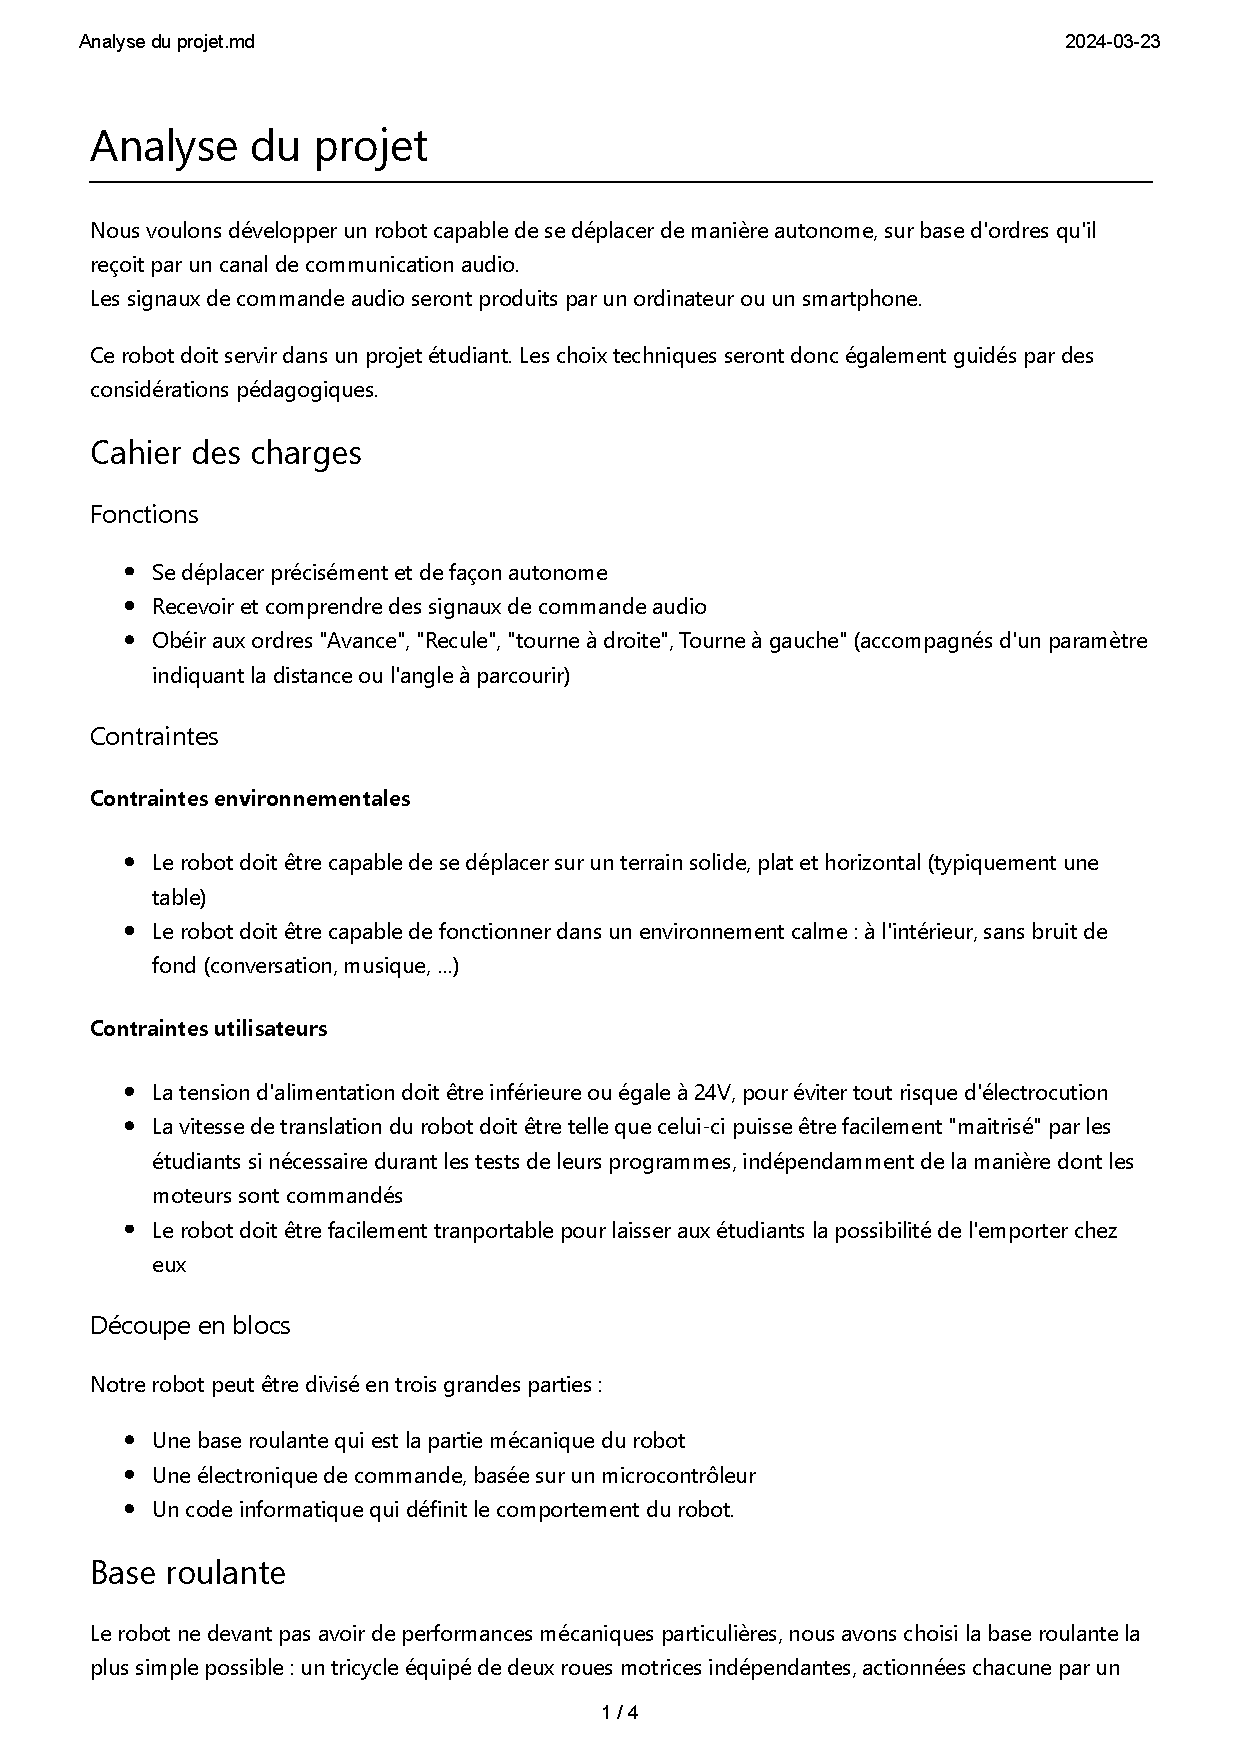
\includepdf[scale=0.5,pages=1,pagecommand={\chapter{Analyse du projet}\label{analyseproj}},linktodoc=true]{pdffiles/Analyse du projet.pdf} 
%\includepdf[scale=0.8,pages=2-]{pdffiles/Analyse du projet.pdf} 

\chapter{Commande mécanique}
%Les pages suivantes proviennent du fichier \textit{Etude deplacement du robot.md} disponible dans le \href{https://gitlab.com/mosee/elech309-2024}{gitlab du projet}
%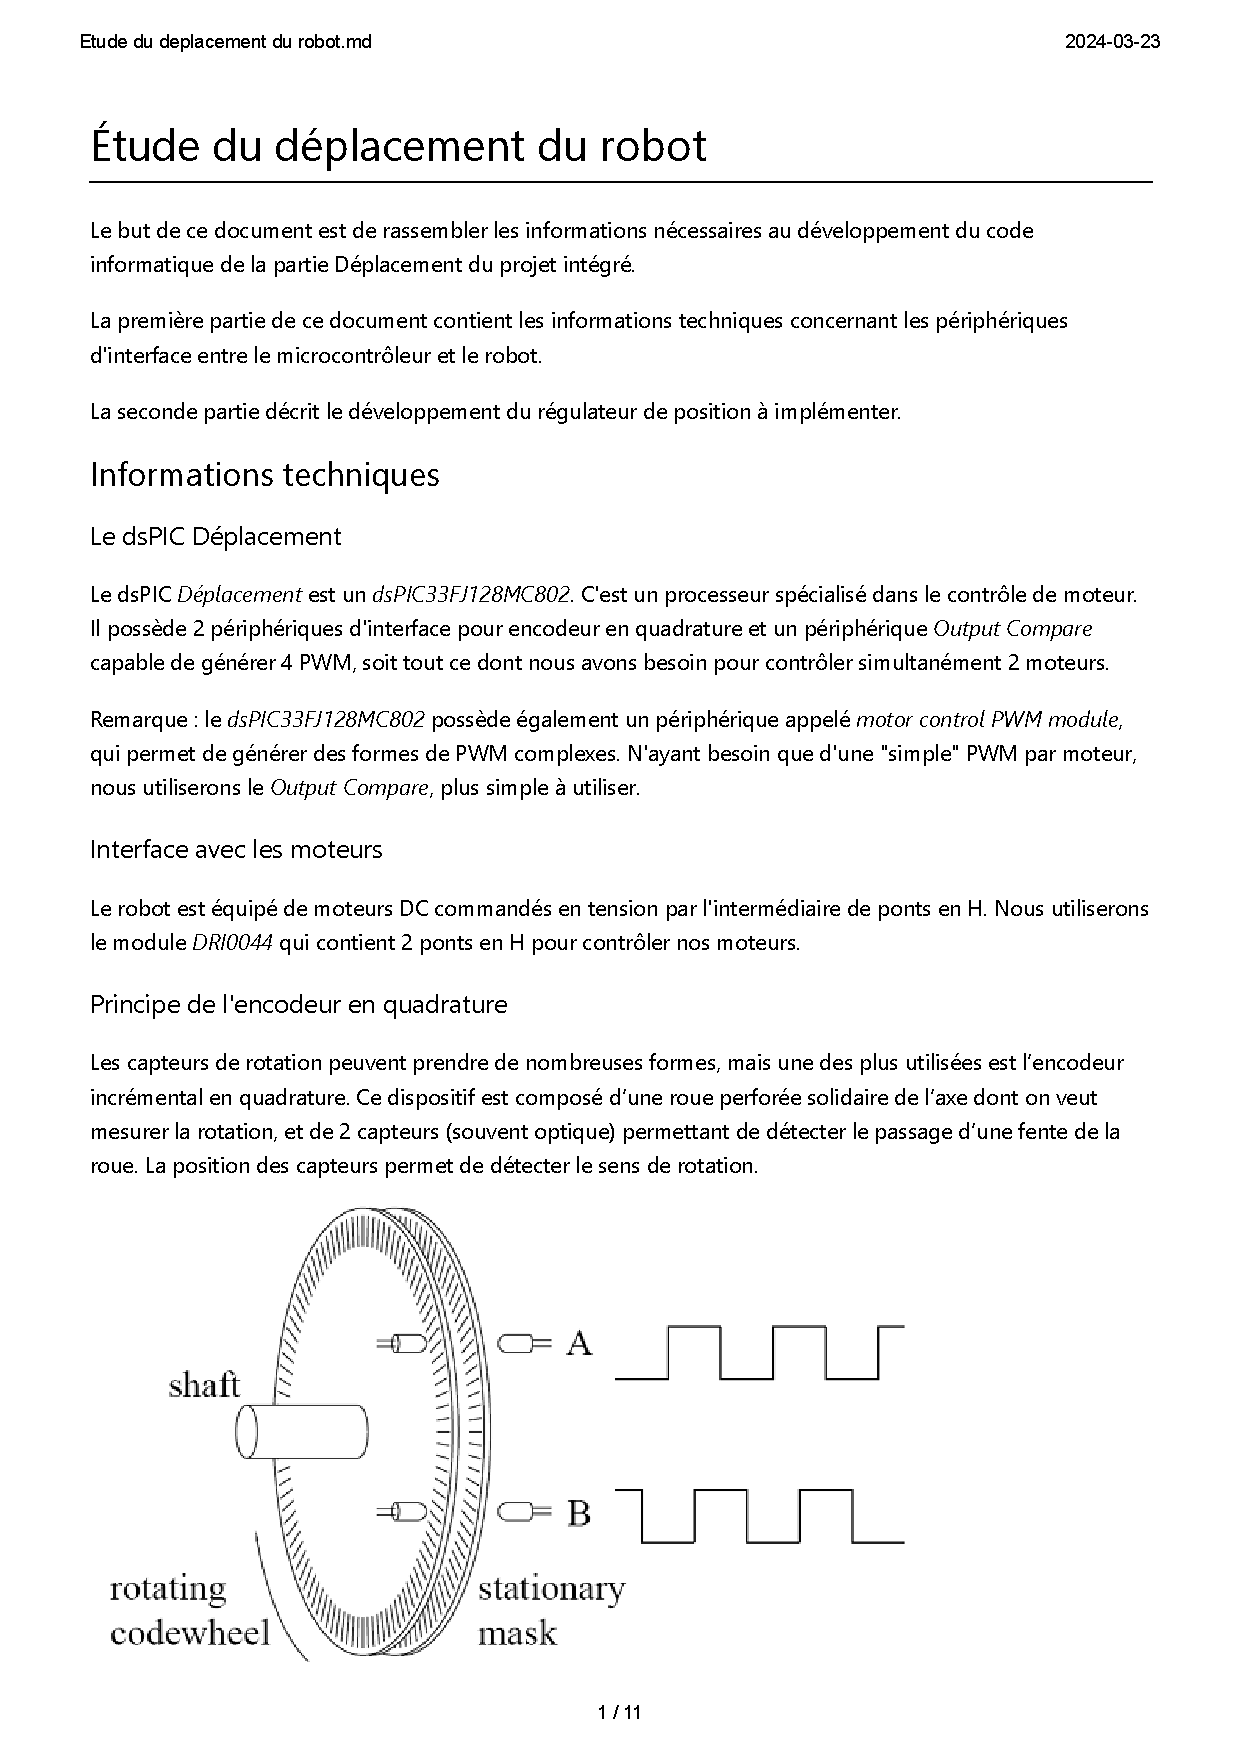
\includepdf[scale=0.8,pages=1,pagecommand={\section{Etude du déplacement du robot }\label{etuderob}},linktodoc=true]{pdffiles/Etude du deplacement du robot.pdf} 
%\includepdf[scale=0.8,pages=2-]{pdffiles/Etude du deplacement du robot.pdf} 
\label{code:mouvement}
\inputminted[breakanywhere=true, breaklines=true, breaksymbol=  ,linenos=true, numberblanklines=false, fontsize=\footnotesize, frame=single, fontfamily=helvetica, autogobble=true,label=\textbf{Code final - mouvement},labelposition=topline]{c}{code/move.c}
\label{code:test_consigne}
\inputminted[breakanywhere=true, breaklines=true, breaksymbol=  ,linenos=true, numberblanklines=false, fontsize=\footnotesize, frame=single, fontfamily=helvetica, autogobble=true,label=\textbf{test - génération de consigne},labelposition=topline]{c}{code/test consigne.c}

\chapter{Traitement des signaux audio}

%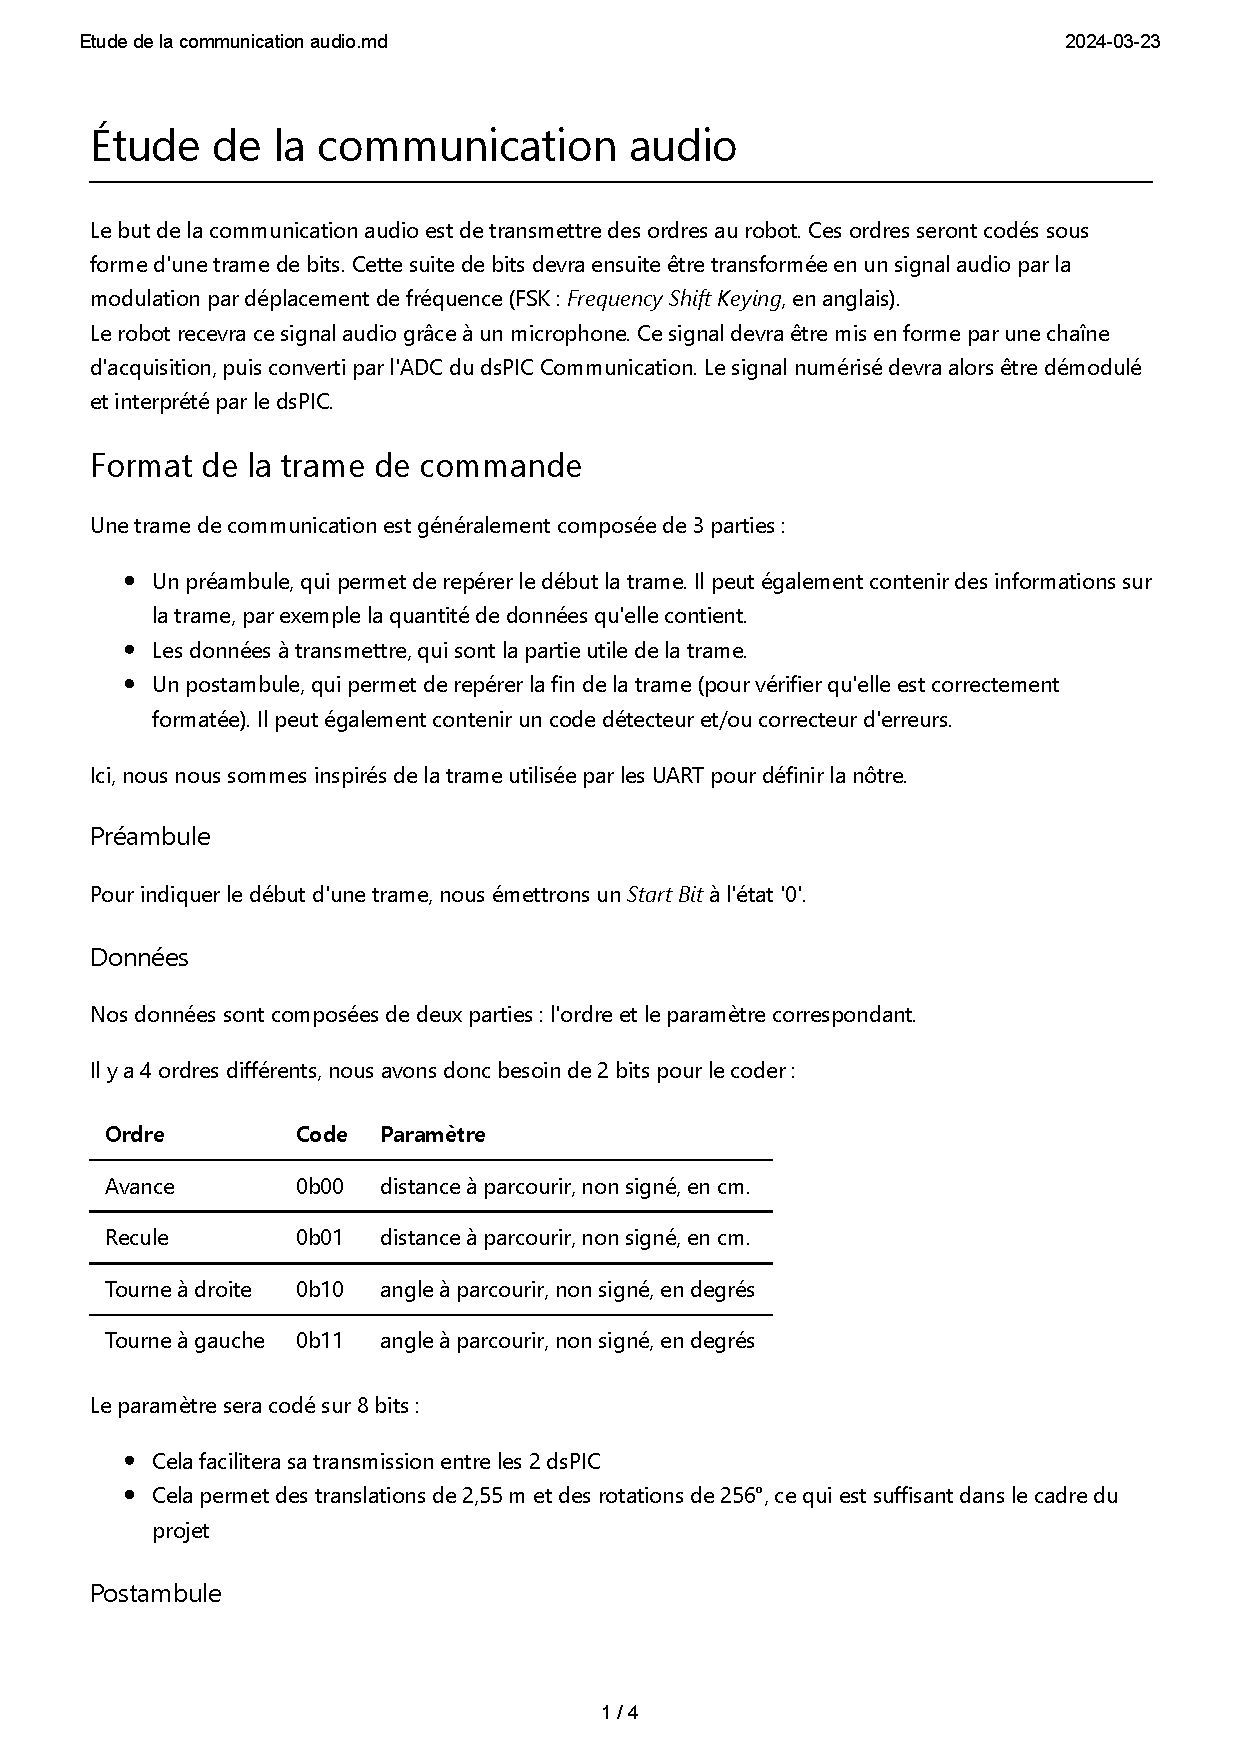
\includepdf[scale=0.8,pages=1,pagecommand={\section{Etude la communication audio}\label{etudecommmd}},linktodoc=true]{pdffiles/Etude de la communication audio.pdf} 
%\includepdf[scale=0.8,pages=2-]{pdffiles/Etude de la communication audio.pdf} 

\section{Filtre passe-haut} \label{hfilterannexe}
\begin{figure}[H]
    \centering
    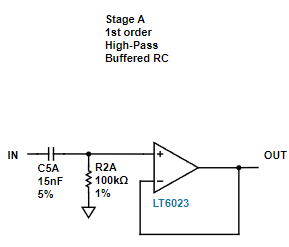
\includegraphics{Pictures/highpassfilter.png}
    \caption{Filtre passe-haut}
    \label{fig:highpassfilterannexe}
\end{figure}


\begin{figure}[H]
    \centering
    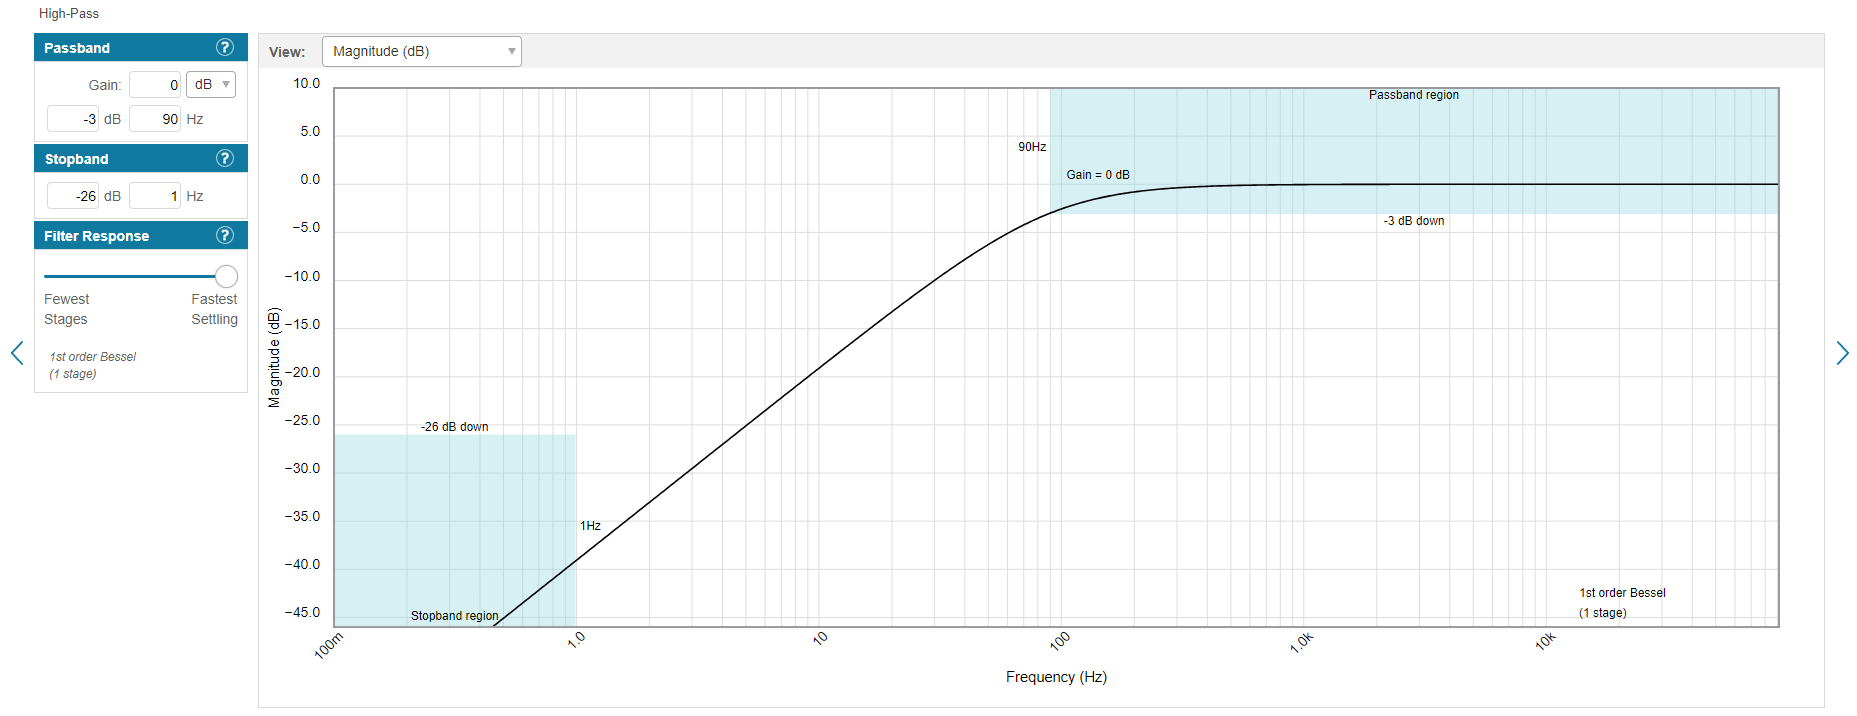
\includegraphics[width=1.5\textwidth,angle=90,origin=c]{Pictures/highpassspecs.png}
    \caption{Gain du filtre passe-haut en dB}
    \label{fig:highpassfiltermagnannexe}
\end{figure}

\newpage
\section{Simulation LTspice du filtre passe-haut avec polarisation} \label{ltspiceHighPassResistors}
\begin{figure}[H]
    \centering
    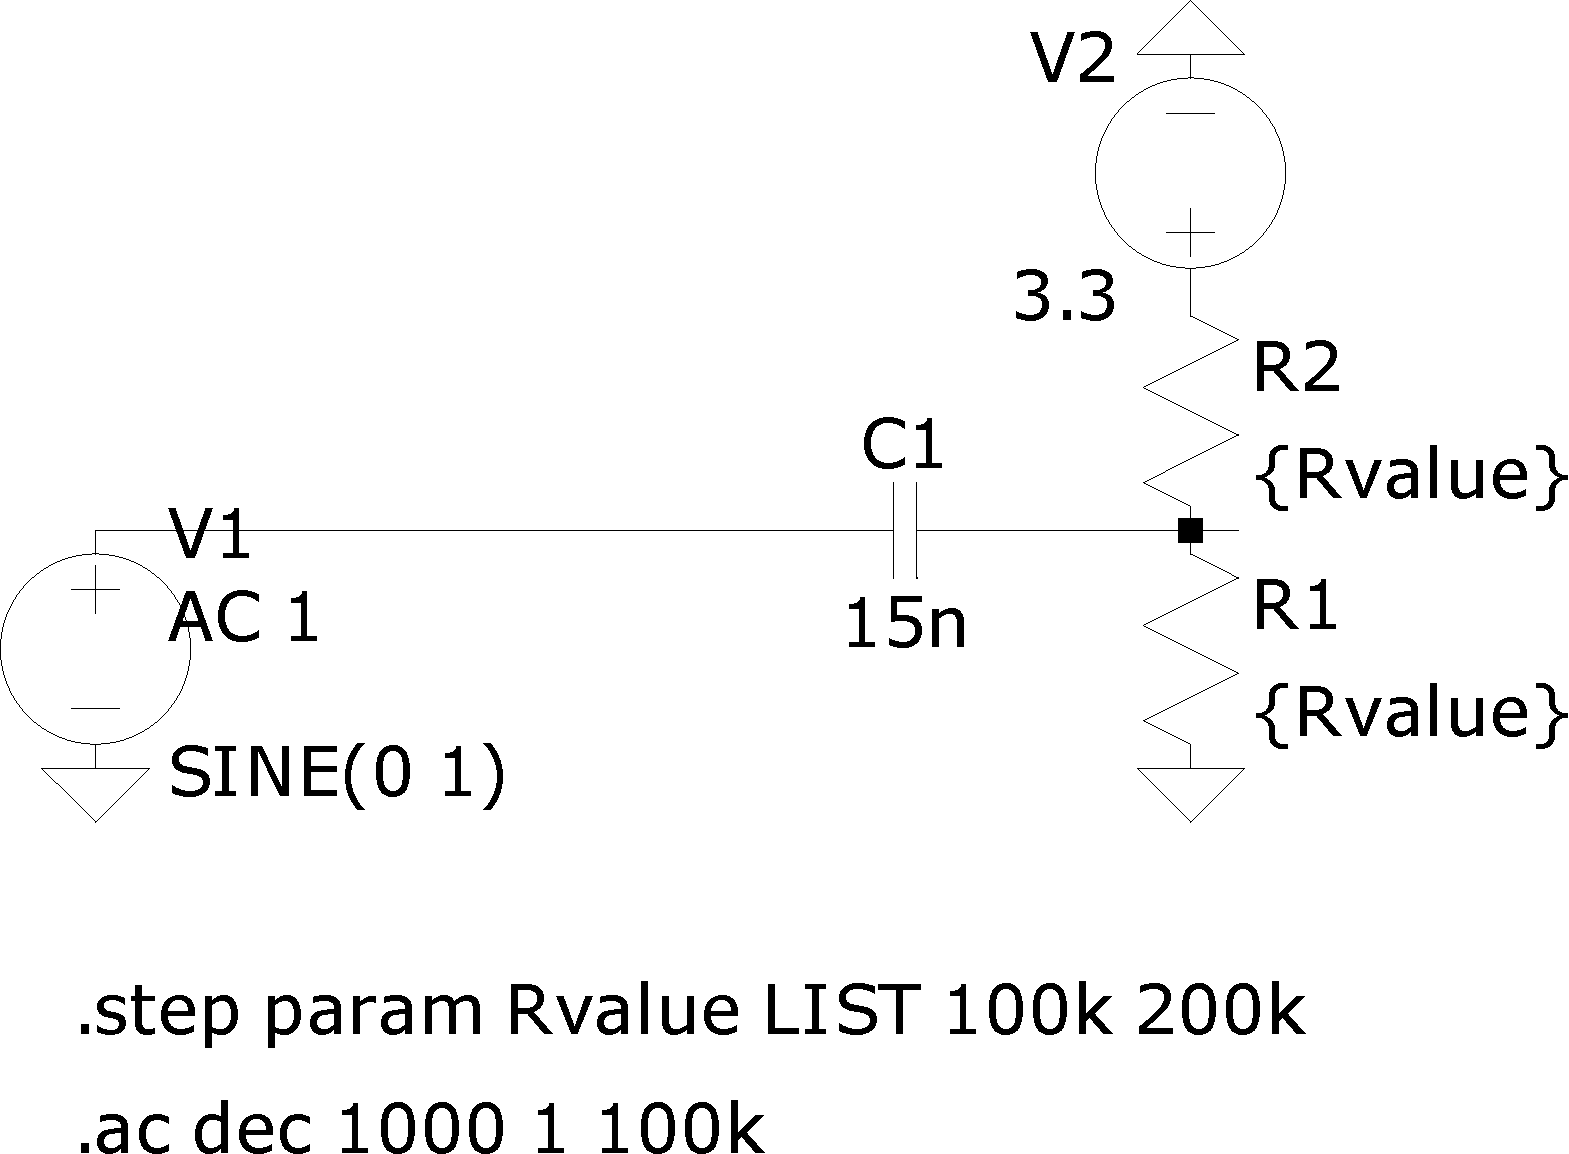
\includegraphics[width=0.7\textwidth]{pdffiles/HighPass/CircuitHighPassPolarization.pdf}
    \caption{Simulation LTspice du filtre passe-haut avec des résistances de polarisation variant de $100k$ à $200k$}
    \label{fig:ltspiceHighPassResistors}
\end{figure}


\includepdf[pages=3,pagecommand={\section{Datasheet MCP601}\label{datasheet}},linktodoc=true]{pdffiles/21314g.pdf}

\newpage
%\section{Comparaison réponse transitoire cas équivalent courant et transistor} \label{LTspiceCurrentvsJFTTransient}
%\begin{figure}[H]
%    \centering
%    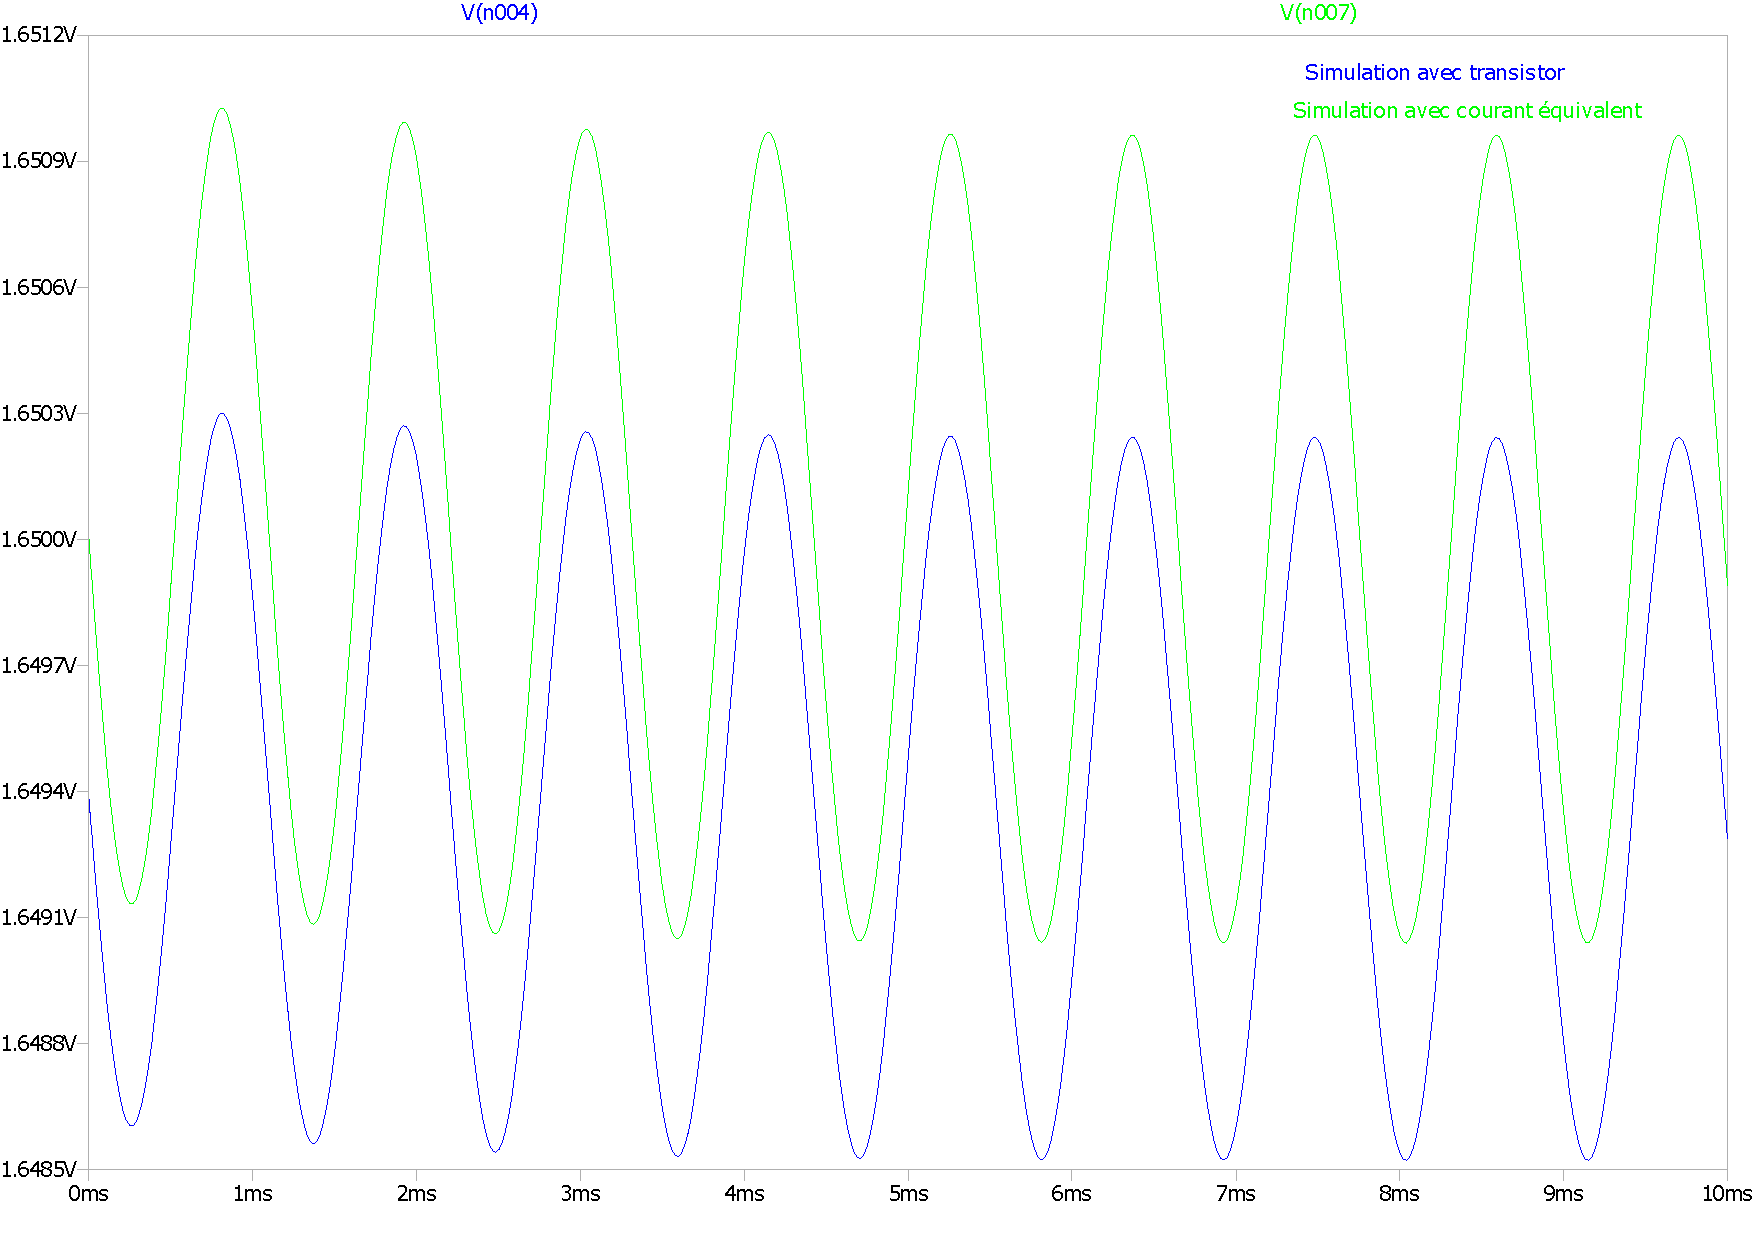
\includegraphics[width=0.7\textwidth]{pdffiles/HighPass/TransientJetVsCurrent.pdf}
%    \caption{Comparaison entre la réponse transitoire du circuit sur la figure \ref{fig:ltspice_current} et celui de la figure \ref{fig:ltspice_transistor}}
%    \label{fig:ltspiceHighPassResistors}
%\end{figure}

\section{Filtre de garde}\label{Lowpassfilterannexe}
\begin{figure}[H]
    \centering
    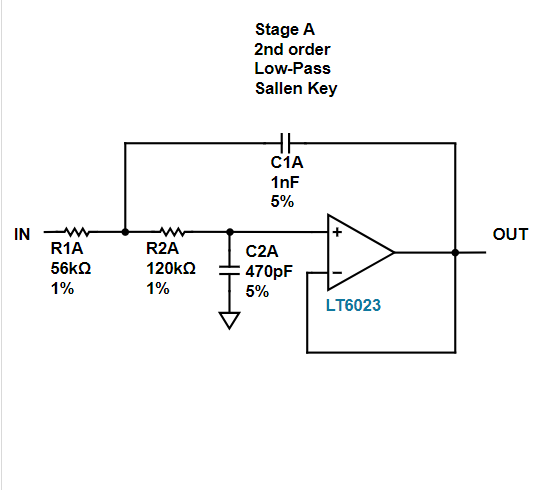
\includegraphics{Pictures/lowpass2.png}
    \caption{Filtre de garde}
    \label{fig:lowpassfilterannexe}
\end{figure}
\newpage
\begin{figure}[H]
    \centering
    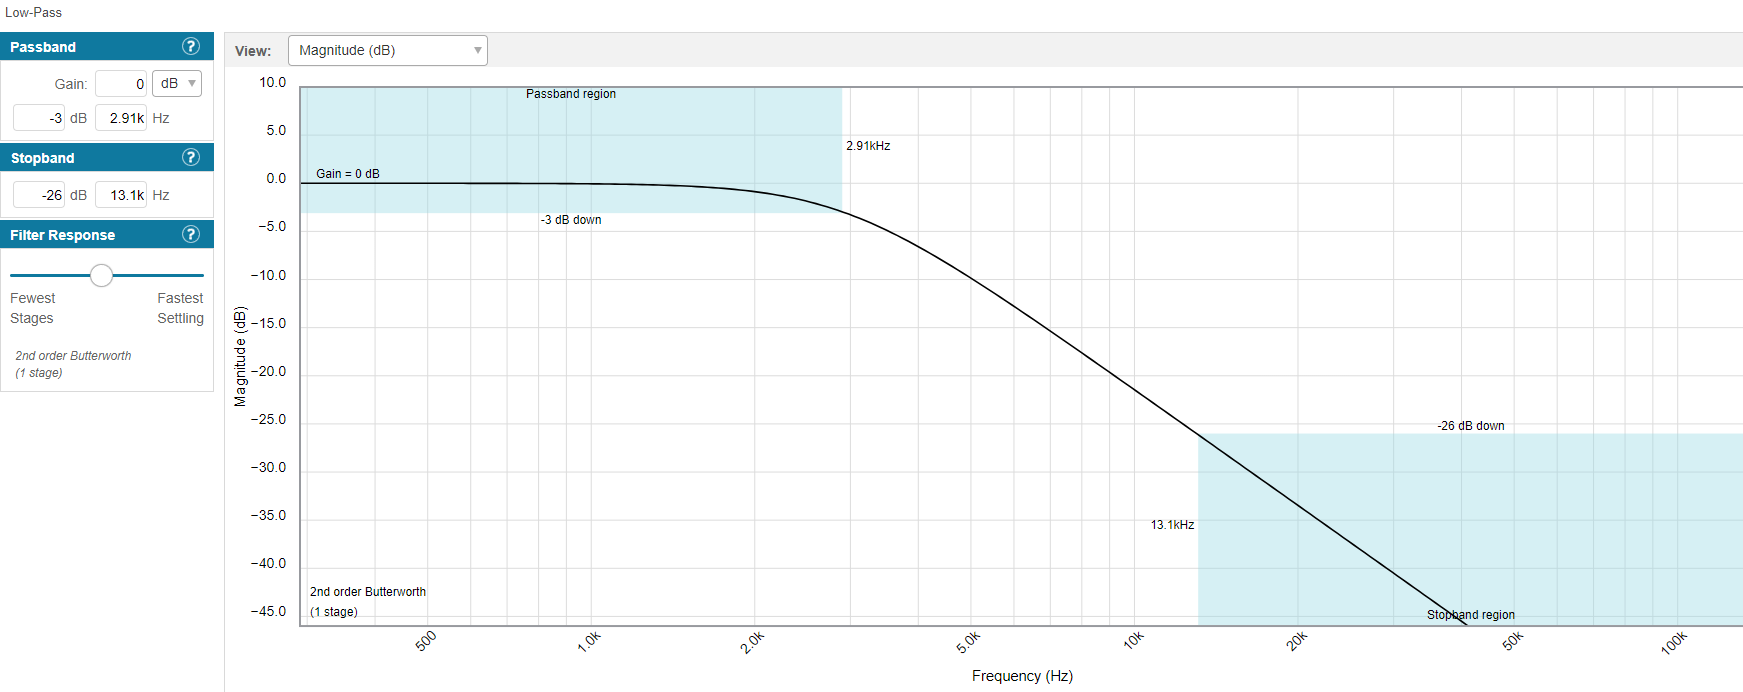
\includegraphics[width=1.5\textwidth,angle=90,origin=c]{Pictures/lowpassspecs.png}
    \caption{Gain du filtre de garde en dB}
    \label{fig:lowpassfiltermagnannexe}
\end{figure}

\section{Circuit de la chaîne d'acquisition}\label{chaineacquiannexe}
\begin{figure}[H]
    \centering
    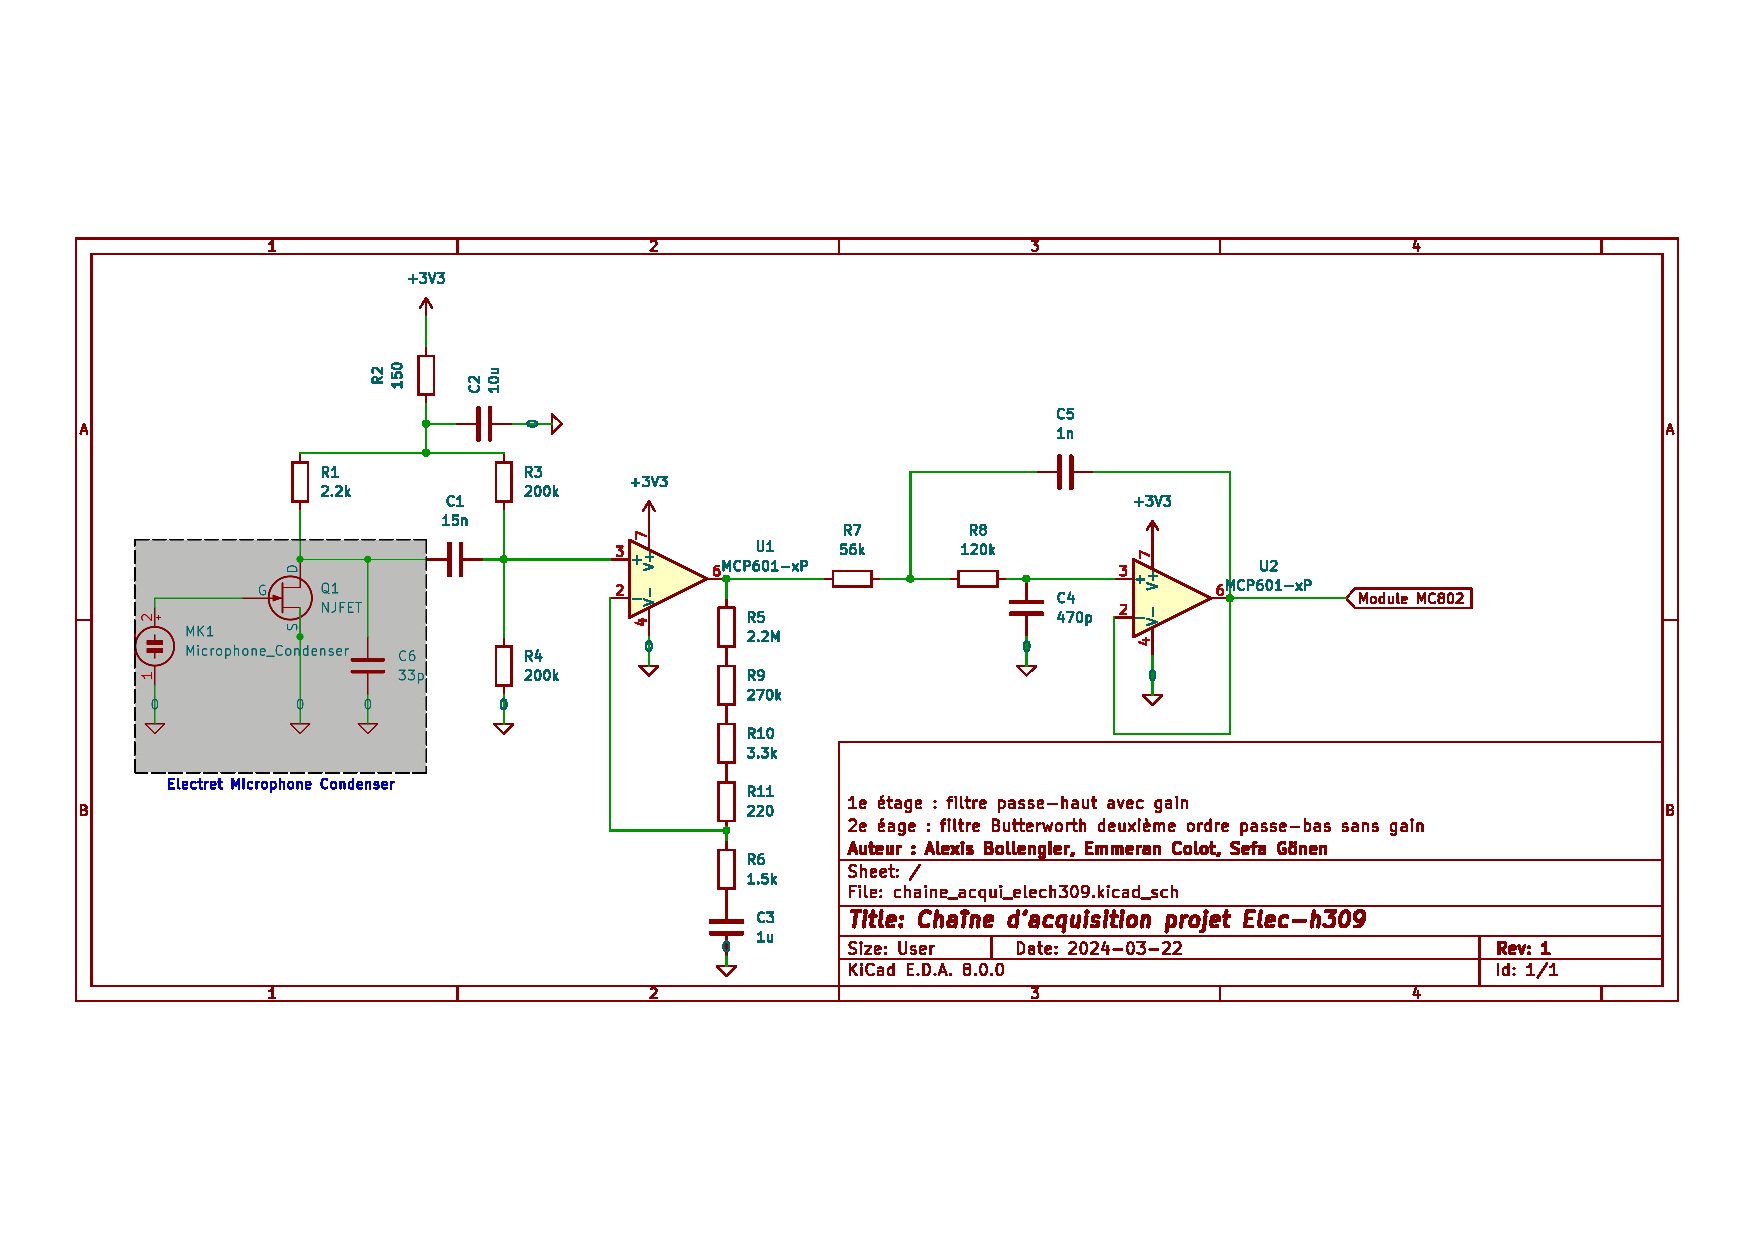
\includegraphics[width=1.4\textwidth,angle=90,origin=c]{pdffiles/chainacquiFullColor.pdf}
    \caption{Circuit de la chaîne d'acquisition}
    \label{fig:chainacquiannexe}
\end{figure}

%\section{Courbes de Bode de la chaîne d'acquisition}\label{Bodechaineacquiannexe}

%\begin{figure}[H]
%    \centering
%    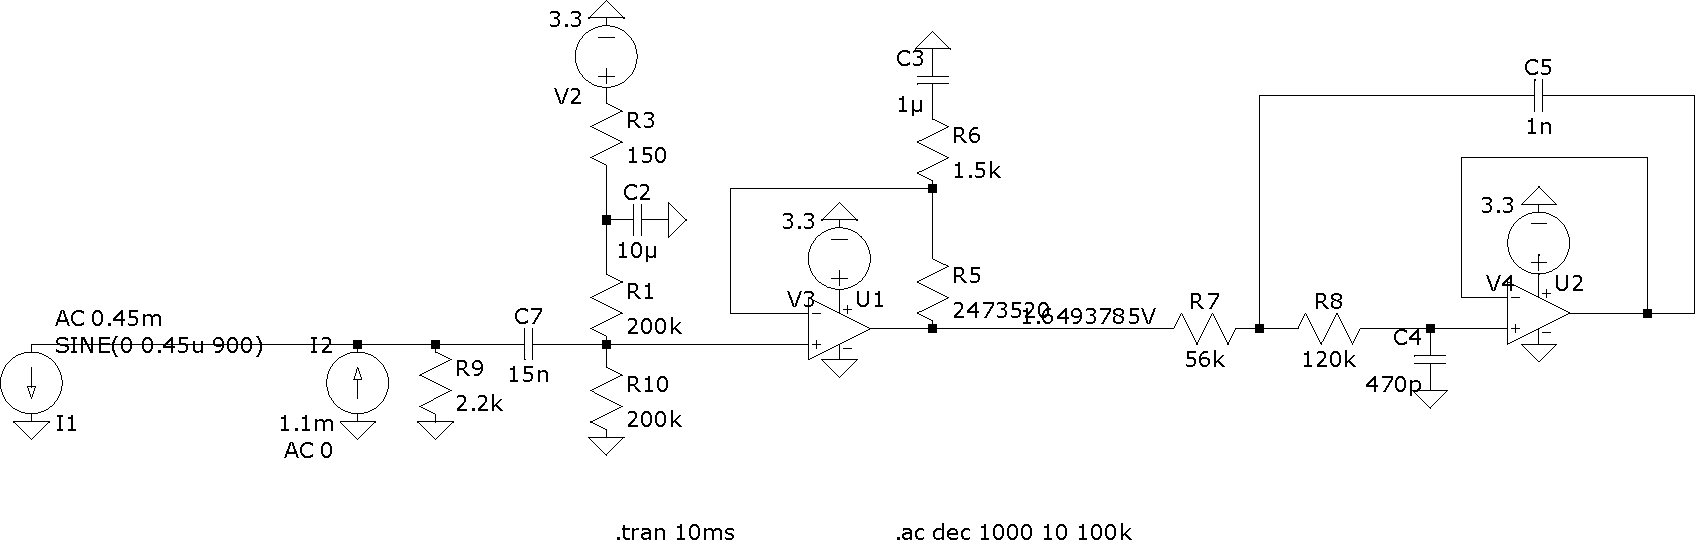
\includegraphics[width=\textwidth]{pdffiles/CircuitCurrent.pdf}
%    \caption{Circuit de simulation LTspice de la chaîne d'acquisition. Le microphone est remplacé par son équivalent source de courant}
%    \label{fig:circuitcurrentannexe}
%\end{figure}
%
%\begin{figure}[H]
%    \centering
%    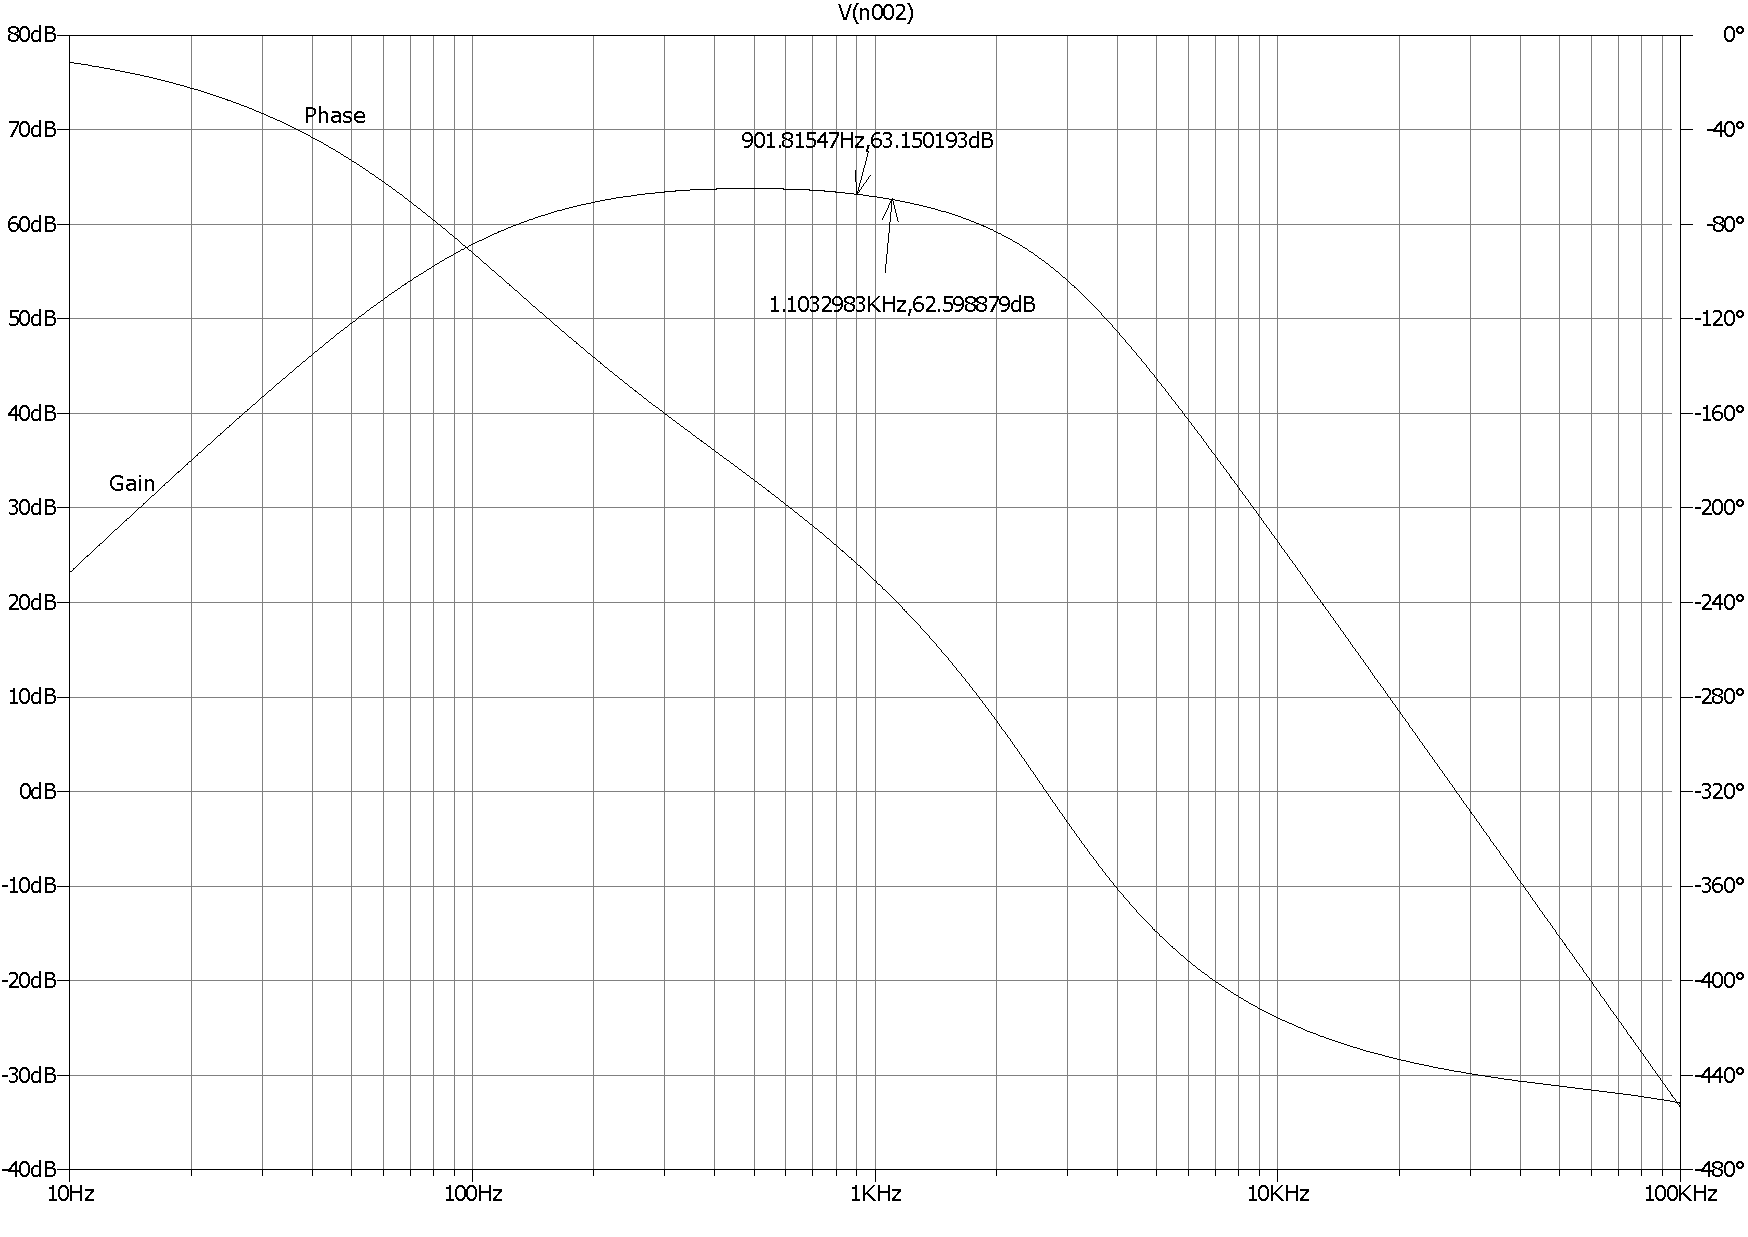
\includegraphics[width=\textwidth]{pdffiles/BodeCircuitCurrent.pdf}
%    \caption{Courbe de Bode de la chaîne d'acquisition. Le microphone est remplacé par son équivalent source de courant}
%    \label{fig:Bodecircuitcurrentannexe}
%\end{figure}
%
%\begin{figure}[H]
%    \centering
%    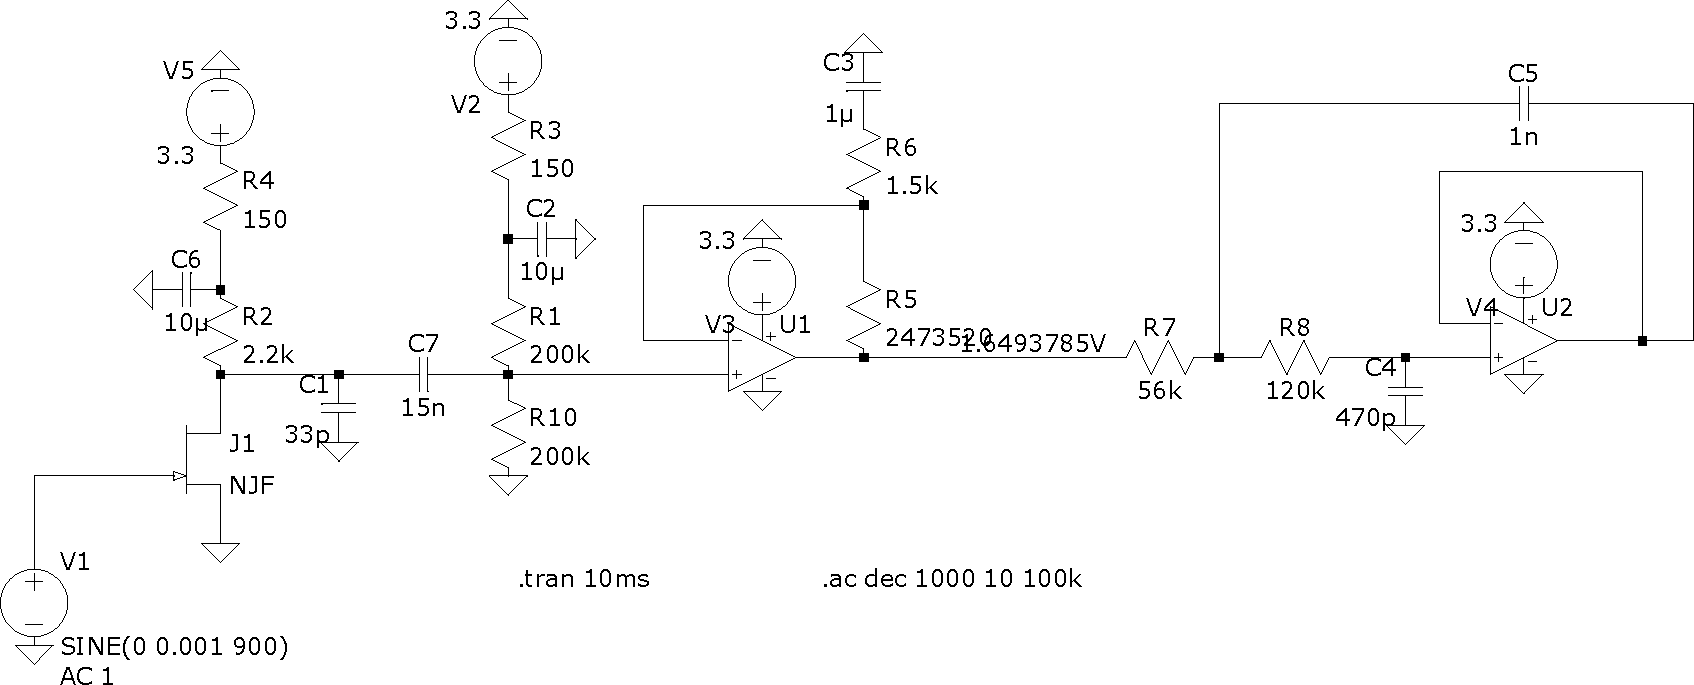
\includegraphics[width=\textwidth]{pdffiles/CircuitJET.pdf}
%    \caption{Circuit de simulation LTspice de la chaîne d'acquisition. Le microphone est remplacé par son équivalent transistor}
%    \label{fig:circuitjetannexe}
%\end{figure}
%
%\begin{figure}[H]
%    \centering
%    \includegraphics[width=\textwidth]{pdffiles/BodeCircuitJET.pdf}
%    \caption{Courbe de Bode de la chaîne d'acquisition. Le microphone est remplacé par son équivalent transistor}
%    \label{fig:Bodecircuitjetannexe}
%\end{figure}

\chapter{Code final}
\label{code:main}
\inputminted[breakanywhere=true, breaklines=true, breaksymbol=  ,linenos=true, numberblanklines=false, fontsize=\footnotesize, frame=single, fontfamily=helvetica, autogobble=true,label=\textbf{Code final - main},labelposition=topline]{c}{code/main.c}


\end{document}